%% LyX 2.1.4 created this file.  For more info, see http://www.lyx.org/.
%% Do not edit unless you really know what you are doing.
\documentclass[ngerman]{article}
\usepackage[T1]{fontenc}
\usepackage[utf8]{inputenc}
\usepackage{refstyle}
\usepackage{float}
\usepackage{mathrsfs}
\usepackage{mathtools}
\usepackage{enumitem}
\usepackage{amsmath}
\usepackage{amsthm}
\usepackage{amssymb}
\usepackage{stmaryrd}

\makeatletter

%%%%%%%%%%%%%%%%%%%%%%%%%%%%%% LyX specific LaTeX commands.

\AtBeginDocument{\providecommand\defref[1]{\ref{def:#1}}}
\AtBeginDocument{\providecommand\lemref[1]{\ref{lem:#1}}}
\RS@ifundefined{subref}
  {\def\RSsubtxt{section~}\newref{sub}{name = \RSsubtxt}}
  {}
\RS@ifundefined{thmref}
  {\def\RSthmtxt{theorem~}\newref{thm}{name = \RSthmtxt}}
  {}
\RS@ifundefined{lemref}
  {\def\RSlemtxt{lemma~}\newref{lem}{name = \RSlemtxt}}
  {}


%%%%%%%%%%%%%%%%%%%%%%%%%%%%%% Textclass specific LaTeX commands.
\usepackage{enumitem}		% customizable list environments
\newlength{\lyxlabelwidth}      % auxiliary length 
\theoremstyle{plain}
\newtheorem{thm}{\protect\theoremname}[section]
  \theoremstyle{definition}
  \newtheorem{defn}[thm]{\protect\definitionname}
% labeling-like list based on enumitem's description list with
% mandatory second argument (label-pattern):
\newenvironment{elabeling}[2][]%
{\settowidth{\lyxlabelwidth}{#2}
\begin{description}[font=\normalfont,style=sameline,
leftmargin=\lyxlabelwidth,#1]}
{\end{description}}
  \theoremstyle{remark}
  \newtheorem*{rem*}{\protect\remarkname}
  \theoremstyle{definition}
  \newtheorem*{example*}{\protect\examplename}
  \theoremstyle{plain}
  \newtheorem{prop}[thm]{\protect\propositionname}
 \newlist{casenv}{enumerate}{4}
 \setlist[casenv]{leftmargin=*,align=left,widest={iiii}}
 \setlist[casenv,1]{label={{\itshape\ \casename} \arabic*.},ref=\arabic*}
 \setlist[casenv,2]{label={{\itshape\ \casename} \roman*.},ref=\roman*}
 \setlist[casenv,3]{label={{\itshape\ \casename\ \alph*.}},ref=\alph*}
 \setlist[casenv,4]{label={{\itshape\ \casename} \arabic*.},ref=\arabic*}
  \theoremstyle{plain}
  \newtheorem{lem}[thm]{\protect\lemmaname}
  \theoremstyle{plain}
  \newtheorem{fact}[thm]{\protect\factname}
  \theoremstyle{plain}
  \newtheorem*{cor*}{\protect\corollaryname}

%%%%%%%%%%%%%%%%%%%%%%%%%%%%%% User specified LaTeX commands.
\usepackage{tikz}
\usepackage{hyperref}

\makeatother

\usepackage{babel}
  \providecommand{\corollaryname}{Korollar}
  \providecommand{\definitionname}{Definition}
  \providecommand{\examplename}{Beispiel}
  \providecommand{\factname}{Fakt}
  \providecommand{\lemmaname}{Lemma}
  \providecommand{\propositionname}{Satz}
  \providecommand{\remarkname}{Bemerkung}
 \providecommand{\casename}{Fall}
\providecommand{\theoremname}{Theorem}

\begin{document}

\section{Einleitung}

Übersicht:
\begin{enumerate}
\item FP{[}<{]} $\subseteq$ SBC ($\subseteq$ P): Jede Fixpunktformel mit
Ordnungsprädikat kann für $n\in\mathbb{N}$ in $\mathrm{poly\left(n\right)}$
in eine FO-Formel auf $n$-Graphen transformiert werden, aus der in
$\mathrm{poly}\left(n\right)$ ein Symmetrischer Boolescher Schaltkreis
wird. Daher ist FP auf P-uniforme SBC-Familien reduzierbar (und diese
auf P).
\item FP+C $\subseteq$ SBC+MAJ ( < P): Majority gates erlauben zusätzlich
Zählterme zu übersetzen.
\item SBC $\subseteq$ FP{[}<{]}: Jede P-uniforme $\left[\sigma\right]$-Schaltkreisfamilie
kann in eine $\mathrm{FP}\left[\sigma+<\right]$-Formel überführt
werden (weil der erzeugende P-Algorithmus per Immerman-Vardi FP{[}<{]}-definierbar
ist). Hierbei ist zu beachten, dass die $<^{\mathfrak{A}}$-Relation
eine beliebige von $\mathfrak{A}$ unabhängige lineare Ordnung ist.
\item SBC+MAJ $\subseteq$ FP+C: FP-Logik mit Zähltermen kann zusätzlich
Majority gates beschreiben.
\item Nicht-uniformes SBC $\subseteq$ FP+C+$\Upsilon$: (Vergleiche mit
,,nicht uniformes AC0 = FO+$\Upsilon$`` aus {[}Anderson, van Melkebeek,
Schweikardt, Segoufin{]}.)
\end{enumerate}
\pagebreak{}


\section{Ergebnisse}


\subsection{Fixpunktlogiken und Schaltkreise}

Es werden die folgenden Äquivalenzen (nach \cite{Anderson2014,anderson_et_al:LIPIcs:2014:4445})
zwischen Fixpunktlogiken und Schaltkreisklassen nachgewiesen:
\begin{thm}
\textbf{$\mathrm{FP}+\mathbf{ORD}$, $P$-uniforme $\mathrm{SBC}$}

Die folgenden Aussagen sind äquivalent:
\begin{enumerate}
\item Die Anfrage $q$ wird durch eine $\left(\mathrm{FP}+\mathbf{ORD}\right)\left[\sigma\right]$-Formel
$\varphi$ definiert.
\item Die Anfrage $q$ wird durch eine $P$-uniforme symmetrische $\left(\sigma,\mathbb{B}_{\mathrm{std}}\right)$-Schaltkreisfamilie
$\mathcal{C}$ berechnet.
\end{enumerate}
\end{thm}
Die Fixpunktlogik mit disjunkter Ordnungserweiterung und Zählterm
ist äquivalent zu den $P$-uniformen symmetrischen booleschen Schaltkreisfamilien
mit Majority-Gates.
\begin{thm}
\textbf{$\mathrm{FP}+C$, $P$-uniforme $\mathrm{SBC}+\mathbf{MAJ}$}

Die folgenden Aussagen sind äquivalent:
\begin{enumerate}
\item Die Anfrage $q$ wird durch eine $\left(\mathrm{FP}+C\right)\left[\sigma\right]$-Formel
$\varphi$ definiert.
\item Die Anfrage $q$ wird durch eine $P$-uniforme symmetrische $\left(\sigma,\mathbb{B}_{\mathrm{maj}}\right)$-Schaltkreisfamilie
$\mathcal{C}$ berechnet.
\end{enumerate}
\end{thm}
Zur Erinnerung: $\mathbb{B}_{\mathrm{maj}}$ enthält die boolesche
Konjunktion, Disjunktion und den Majority-Operator $\mathrm{MAJ}=\left\{ \left(m,n\right)\mid m\leqslant n\right\} $.


\begin{thm}
\textbf{$\mathrm{FP}+\Upsilon$, $\mathrm{poly\left(n\right)}$-große
$\mathrm{SBC}$}

Die folgenden Aussagen sind äquivalent:
\begin{enumerate}
\item Die Anfrage $q$ wird durch eine $\left(\mathrm{FP}+\Upsilon\right)\left[\sigma\right]$-Formel
$\varphi$ definiert.
\item Die Anfrage $q$ wird durch eine $\mathrm{poly}\left(n\right)$-große
symmetrische $\left(\sigma,\mathbb{B}_{\mathrm{std}}\right)$-Schaltkreisfamilie
$\mathcal{C}$ berechnet.
\end{enumerate}
\end{thm}
Zur Erinnerung: $\mathbb{B}_{\mathrm{maj}}$ enthält die boolesche
Konjunktion, Disjunktion und den Majority-Operator $\mathrm{MAJ}=\left\{ \left(m,n\right)\mid m\leqslant n\right\} $.


\begin{thm}
\textbf{$\mathrm{FP}+\Upsilon+C$, $\mathrm{poly}\left(n\right)$-große
$\mathrm{SBC}+\mathbf{MAJ}$}

Die folgenden Aussagen sind äquivalent:
\begin{enumerate}
\item Die Anfrage $q$ wird durch eine $\left(\mathrm{FP}+\Upsilon+C\right)\left[\sigma\right]$-Formel
$\varphi$ definiert.
\item Die Anfrage $q$ wird durch eine $\mathrm{poly}\left(n\right)$-große
symmetrische $\left(\sigma,\mathbb{B}_{\mathrm{maj}}\right)$-Schaltkreisfamilie
$\mathcal{C}$ berechnet.
\end{enumerate}
\end{thm}
eine Orakelfunktion, die jeder Zahl $n$ die Orakelstruktur $\mathbf{ARB}\left(n\right)=\mathfrak{N}_{\mid\left\{ 0,\cdots,n\right\} }$
zuweist.

Für jede $\mathrm{FO}+\mathbf{ARB}$-Formel $\varphi$ existiert eine
arb-invariante $\mathrm{FO}\left[\sigma_{\mathrm{arb}}\right]$-Formel
$\varphi'$, die auf allen endlichen $\sigma$-Strukturen äquivalent
zu $\varphi$ ist, und umgekehrt.


\subsection{Logik erster Stufe und Schaltkreise konstanter Tiefe}
\begin{thm}
\cite{IMMERMAN198686}\label{thm:5.5:fo-ord}$\mathrm{FO}+\mathbf{ORD}$,
$P$-uniformes symmetrisches $\mathrm{AC}^{0}$.

Die folgenden Aussagen sind äquivalent:
\begin{enumerate}
\item Die Anfrage $q$ wird durch eine $\left(\mathrm{FO}+\mathbf{ORD}\right)\left[\sigma\right]$-Formel
$\varphi$ definiert.
\item Die Anfrage $q$ wird durch eine $P$-uniforme, $\mathcal{O}\left(1\right)$-tiefe,
symmetrische $\left(\sigma,\mathbb{B}_{\mathrm{std}}\right)$-Schaltkreisfamilie
$\mathcal{C}$ berechnet.
\end{enumerate}
\end{thm}

\begin{thm}
\label{thm:5.6:fo-c}$\mathrm{FO}+C$, symmetrisches $\mathrm{AC}^{0}+\mathbf{MAJ}$.

Die folgenden Aussagen sind äquivalent:
\begin{enumerate}
\item Die Anfrage $q$ wird durch eine $\left(\mathrm{FO}+C\right)\left[\sigma\right]$-Formel
$\varphi$ definiert.
\item Die Anfrage $q$ wird durch eine $\mathcal{O}\left(1\right)$-tiefe,
$\mathrm{poly}\left(n\right)$-große, symmetrische $\left(\sigma,\mathbb{B}_{\mathrm{maj}}\right)$-Schaltkreisfamilie
$\mathcal{C}$ berechnet.
\end{enumerate}
\end{thm}

\begin{thm}
\label{thm:5.7:fo+u}$\mathrm{FO}+\Upsilon$, symmetrisches $\mathrm{AC}^{0}$.

Die folgenden Aussagen sind äquivalent:
\begin{enumerate}
\item Die Anfrage $q$ wird durch eine $\left(\mathrm{FO}+\Upsilon\right)\left[\sigma\right]$-Formel
$\varphi$ definiert.
\item Die Anfrage $q$ wird durch eine $\mathcal{O}\left(1\right)$-tiefe,
$\mathrm{poly}\left(n\right)$-große, symmetrische $\left(\sigma,\mathbb{B}_{\mathrm{std}}\right)$-Schaltkreisfamilie
$\mathcal{C}$ berechnet.\end{enumerate}
\begin{thm}
$\mathrm{FO}+\Upsilon+C$, symmetrisches $\mathrm{AC}^{0}+\mathbf{MAJ}$.

Die folgenden Aussagen sind äquivalent:
\begin{enumerate}
\item Die Anfrage $q$ wird durch eine $\left(\mathrm{FO}+\Upsilon\right)\left[\sigma\right]$-Formel
$\varphi$ definiert.
\item Die Anfrage $q$ wird durch eine $\mathcal{O}\left(1\right)$-tiefe,
$\mathrm{poly}\left(n\right)$-große, symmetrische $\left(\sigma,\mathbb{B}_{\mathrm{maj}}\right)$-Schaltkreisfamilie
$\mathcal{C}$ berechnet.
\end{enumerate}
\end{thm}
\end{thm}

\subsection{Logik erster Stufe mit disjunktem und nicht-disjunktem Orakel}
\begin{thm}
$\mathrm{FO}+\Upsilon$, invariantes $\mathrm{FO}\left(\mathrm{arb}\right)$
\begin{enumerate}
\item Jede $\left(\mathrm{FO}+\Upsilon\right)\left[\sigma\right]$-Formel
$\varphi$ ist äquivalent zu einer arb-invarianten $\mathrm{FO}\left[\sigma_{\mathrm{arb}}\right]$-Formel
$\varphi$.
\item Es existiert eine $\sigma$-Anfrage, die in der arb-invarianten $\mathrm{FO}\left[\sigma_{\mathrm{arb}}\right]$-Logik
definierbar ist, aber nicht $\left(\mathrm{FO}+\Upsilon\right)\left[\sigma\right]$-definierbar
ist.
\end{enumerate}
\end{thm}
\pagebreak{}


\section{Grundlagen}

Diese Arbeit verwendet verschiedene Begriffe der endlichen Modelltheorie
und der Graphentheorie. Diese Begriffe werden im folgenden formal
definiert.


\subsection{Notationen}
\begin{defn}
\textbf{Tupel}

Ein Tupel $\left(x_{1},\cdots,x_{n}\right)$ von Elementen einer Menge
$U$ wird durch $\bar{x}\in U^{n}$ notiert.

Die \textbf{Stelligkeit} $\mathrm{ar}\left(\bar{x}\right)$ eines
Tupels $\bar{x}$ sei die Anzahl seiner Elemente, und ein $n$-stelliges
Tupel heiße kurz ,,$n$-Tupel``.

Für ein $m$-Tupel $\bar{x}$ und ein $n$-Tupel $\bar{y}$ sei $\bar{x}\bar{y}$
das $\left(m+n\right)$-Tupel $\left(x_{1},\cdots,x_{m},y_{1},\cdots,y_{n}\right)$.

Das $0$-stellige Tupel wird durch $\left\langle \right\rangle $
notiert.
\end{defn}

\begin{defn}
\textbf{Relation}

Für eine Menge $A$ und $k\in\mathbb{N}$ sei $R\subseteq A^{k}$
eine $k$-stellige Relation über $A$. Sei $2^{A}=\left\{ A'\mid A'\subseteq A\right\} $
die Potenzmenge von $A$.

Für jede Relation $R\subseteq A^{k}$ sei $\left[R\right]:A^{k}\rightarrow\left\{ 0,1\right\} $
die folgende Funktion: 
\[
\left[R\right]\left(\bar{a}\right)\coloneqq\begin{cases}
1 & \mathrm{falls}\,\,\bar{a}\in R\\
0 & \mathrm{sonst}
\end{cases}
\]
 
\end{defn}

\begin{defn}
\textbf{Intervall}

Die Menge $\left\{ i\in\mathbb{N}\mid a\leqslant i\leqslant b\right\} $
wird durch $\left[a,b\right]$ abgekürzt.
\end{defn}

\begin{defn}
\textbf{Abbildung}

Für eine Abbildung $\pi:A\rightarrow B$ und $a\in A$ wird $\pi\left(a\right)$
auch durch $\pi a$ abgekürzt.

Es sei $\mathbf{id}:A\rightarrow A$ die Identität mit $\mathbf{id}\left(a\right)=a$
für alle $a\in A$.

Jede Abbildung $\pi:A\rightarrow B$ wird auf natürliche Weise auf
Tupel, Teilmengen und Relationen von $A$ erweitert:
\begin{eqnarray*}
\pi\left(x_{1},\cdots,x_{k}\right) & \coloneqq & \left(\pi x_{1},\cdots,\pi x_{n}\right)\\
\pi\left\{ x_{1},\cdots,x_{n}\right\}  & \coloneqq & \left\{ \pi x_{1},\cdots,\pi x_{n}\right\} \\
\pi\left\{ \left(x_{1,1},\cdots,x_{1,k}\right),\cdots,\left(x_{n,1},\cdots,x_{n,k}\right)\right\}  & \coloneqq & \left\{ \left(\pi x_{1,1},\cdots,\pi x_{1,k}\right),\cdots,\left(\pi x_{n,1},\cdots,\pi x_{n,k}\right)\right\} 
\end{eqnarray*}


Eine Abbildung $\pi:\left\{ a_{1},\cdots,a_{n}\right\} \rightarrow B$
wird extensional durch $\left(\begin{array}{c}
a_{1}\\
\pi a_{1}
\end{array}\cdots\begin{array}{c}
a_{n}\\
\pi a_{n}
\end{array}\right)$ notiert.

Für zwei Abbildungen $\pi_{1}:B\rightarrow C$ und $\pi_{2}:A\rightarrow B$
sei $\pi_{1}\circ\pi_{2}:A\rightarrow C$ (kurz $\pi_{1}\pi_{2}$)
die folgende Abbildung: 
\[
\pi_{1}\pi_{2}\coloneqq\left(\begin{array}{c}
a_{1}\\
\pi_{1}\left(\pi_{2}\left(a_{1}\right)\right)
\end{array}\cdots\begin{array}{c}
a_{n}\\
\pi_{1}\left(\pi_{2}\left(a_{n}\right)\right)
\end{array}\right)
\]


Für zwei Abbildungen $\pi:A\rightarrow B$ und $\pi':A'\rightarrow B'$
mit disjunkten Definitionsbereichen sei $\pi\cup\pi':A\uplus A'\rightarrow B\cup B'$
die folgende Abbildung:
\[
\left(\pi\cup\pi'\right)x\coloneqq\begin{cases}
\pi x & \mathrm{falls}\,\,x\in A\\
\pi'x & \mathrm{falls}\,\,x\in A'
\end{cases}
\]


Für $\pi:A\rightarrow B$ und $A'\subseteq A$ sei $\pi_{\mid A'}:A'\rightarrow B$
die Reduktion auf eine Teilmenge des Definitionsbereichs, und $\pi_{\backslash A'}:A\backslash A'\rightarrow B$
die Reduktion auf das Komplement.
\end{defn}

\begin{defn}
\textbf{Permutation}

Eine Permutation von $U$ ist eine bijektive Abbildung $\pi:U\rightarrow U$.

Die Menge aller Permutationen von $U$ sei $\mathrm{Sym}_{U}$; diese
bilden eine Symmetrie-Gruppe bezüglich der Verkettung $\circ:\mathrm{Sym}_{U}\times\mathrm{Sym}_{U}\rightarrow\mathrm{Sym}_{U}$
mit dem neutralen Element $\mathbf{id}$.

Es sei $\pi^{-1}$ die inverse Abbildung mit $\pi^{-1}\pi=\pi\pi^{-1}=\mathbf{id}$.

Eine Transposition sei eine Permutation, die zwei Elemente $u_{i}$
und $u_{j}$ vertauscht und alle anderen Elemente fixiert. Diese wird
kurz durch $\left(u_{i}u_{j}\right)$ notiert.
\end{defn}

\subsection{Relationale Strukturen}

Wir betrachten Anfragen und Eigenschaften auf Graphen und allgemeinen
relationalen Strukturen.
\begin{defn}
\textbf{Relationale Signatur}

Eine relationale Signatur $\sigma$ ist eine Menge von Relationssymbolen.
Jedes Symbol $R\in\sigma$ hat eine feste Stelligkeit $\mathrm{ar}\left(R\right)=k\in\mathbb{N}_{\geqslant1}$.
Gegebenenfalls wird die Stelligkeit kompakt durch $R/k\in\sigma$
notiert.
\end{defn}

\begin{defn}
\textbf{Endliche Struktur}

Eine endliche $\sigma$-Struktur $\mathfrak{A}=\left(A,\left(R^{\mathfrak{A}}\right)_{R\in\sigma}\right)$
besteht aus einem endlichen, nicht-leeren Universum $A$ und einer
Interpretation $R^{\mathfrak{A}}\subseteq A^{k}$ für jedes Symbol
$R/k\in\sigma$.

Wir formalisieren die Interpretation als eine Abbildung $\square^{\mathfrak{A}}:\sigma\rightarrow\bigcup_{k\in\mathbb{N}}2^{\left(A^{k}\right)}$,
die jedem Symbol eine Relation der entsprechenden Stelligkeit zuweist.
Damit kann die Interpretation gegebenenfalls auch explizit durch $\mathfrak{A}=\left(A,\square^{\mathfrak{A}}\right)$
notiert werden, um die Zuordnung von Symbolen und Relationen zu verdeutlichen:
\[
\mathfrak{A}:=\left(A,\left(\begin{array}{ccc}
R_{1} & \cdots & R_{k}\\
R_{1}^{\mathfrak{A}} & \cdots & R_{k}^{\mathfrak{A}}
\end{array}\right)\right)
\]

\begin{enumerate}
\item Für eine endliche Menge $U$ sei $\mathbf{FIN}^{U}\left(\sigma\right)$
die Menge aller $\sigma$-Strukturen über dem Universum $U$.
\item Für $n\in\mathbb{N}_{\geqslant1}$ seien $\mathbf{FIN}^{\left(n\right)}\left(\sigma\right)$
die $\sigma$-Strukturen über einem beliebigen Universum der Größe
$n$.
\item Seien $\mathbf{FIN}\left(\sigma\right)\coloneqq\bigcup_{n\in\mathbb{N}_{\geqslant1}}\mathbf{FIN}^{\left(n\right)}\left(\sigma\right)$
die endlichen $\sigma$-Strukturen.
\end{enumerate}
\end{defn}

\begin{defn}
\textbf{Geordnete Struktur}

Sei $\sigma$ eine relationale Signatur, die nicht das zweistellige
Symbol $\leqslant$ enthält.

Für $a,b\in\mathbb{N}$ seien $\mathbf{FIN}_{\leqslant}^{\left[a,b\right]}\left(\sigma\right)\subseteq\mathbf{FIN}^{\left[a,b\right]}\left(\sigma\cup\left\{ \leqslant\right\} \right)$
die endlichen $\sigma\cup\left\{ \leqslant\right\} $-Strukturen über
$\left[a,b\right]$, wobei $\leqslant$ durch die natürliche Ordnung
von $\left[a,b\right]$ interpretiert wird, und sei $\mathbf{FIN}_{\leqslant}\left(\sigma\right)\coloneqq\bigcup_{a,b\in\mathbb{N}}\mathbf{FIN}_{\leqslant}^{\left[a,b\right]}\left(\sigma\right)$
die Klasse aller endlichen geordneten $\sigma\cup\left\{ \leqslant\right\} $-Strukturen. 

Der Lesbarkeit halber wird die Infixnotation $a\leqslant b$ anstelle
von $\left(a,b\right)\in\leqslant$ oder $\leqslant\left(a,b\right)$
verwendet.

Die Symbole $\dot{\leqslant}$ und $\dot{=}$ seien gleichbedeutend
mit den Symbolen $\leqslant$ und $=$, und werden der Lesbarkeit
halber in Gleichungen wie $\varphi=x\dot{=}y$ und $\varphi=x\dot{\leqslant}y$
verwendet.
\end{defn}

\begin{defn}
\textbf{\label{def:Isomorphismus}Isomorphismus}

Für zwei $\sigma$-Strukturen $\mathfrak{A}$ und $\mathfrak{B}$
sei eine bijektive Abbildung $\pi:A\rightarrow B$ ein Isomorphismus,
falls $\pi R^{\mathfrak{A}}=R^{\mathfrak{B}}$ für alle Symbole $R\in\sigma$
gilt.

Die Abbildung $\pi$ wird auf natürliche Weise auf Strukturen erweitert:
\[
\pi\mathfrak{A}\coloneqq\left(\pi A,\left(\pi R^{\mathfrak{A}}\right)_{R\in\sigma}\right)
\]


Der Isomorphismus wird kurz durch $\pi:\mathfrak{A}\tilde{\rightarrow}\mathfrak{B}$
notiert. Zwei Strukturen heißen isomorph (kurz $\mathfrak{A}\cong\mathfrak{B}$),
falls ein $\pi:\mathfrak{A}\tilde{\rightarrow}\mathfrak{B}$ existiert.

Ein Automorphismus $\pi:\mathfrak{A}\tilde{\rightarrow}\mathfrak{A}$
sei ein Isomorphismus von $\mathfrak{A}$ zu sich selbst. Die Menge
aller Automorphismen von $\mathfrak{A}$ sei $\mathrm{Aut}_{\mathfrak{A}}$;
diese bilden wiederum eine Gruppe bezüglich $\circ$ und dem neutralen
Element $\mathbf{id}$.
\end{defn}

\begin{defn}
\textbf{\label{def:Disjunkte-Vereinigung}Vereinigung von Strukturen}

Zwei Strukturen können vereinigt werden, wenn sie entweder disjunkte
Signaturen oder die gleiche Signatur besitzen. Für eine $\sigma_{1}$-Struktur
$\mathfrak{A}$ und eine $\sigma_{2}$-Struktur $\mathfrak{B}$ gilt:
\begin{enumerate}
\item Wenn $\sigma_{1}\cap\sigma_{2}=\emptyset$, so ist $\mathfrak{A}\cup\mathfrak{B}$
die folgende $\left(\sigma_{1}\cup\sigma_{2}\right)$-Struktur:
\[
\mathfrak{A}\cup\mathfrak{B}\coloneqq\left(A\cup B,\left(R^{\mathfrak{A}}\right)_{R\in\sigma_{1}},\left(R^{\mathfrak{B}}\right)_{R\in\sigma_{2}}\right)
\]

\item Wenn $\sigma_{1}=\sigma_{2}=\sigma$, so ist $\mathfrak{A}\cup\mathfrak{B}$
die folgende $\sigma$-Struktur:
\[
\mathfrak{A}\cup\mathfrak{B}\coloneqq\left(A\cup B,\left(R^{\mathfrak{A}}\cup R^{\mathfrak{B}}\right)_{R\in\sigma}\right)
\]

\end{enumerate}
Falls das Universum der beiden Strukturen ebenfalls disjunkt ist,
so heißt $\mathfrak{A}\cup\mathfrak{B}=\mathfrak{A}\uplus\mathfrak{B}$
die \textbf{disjunkte Vereinigung} der Strukturen.
\end{defn}

\begin{defn}
\textbf{\label{def:Induzierte-Teilstruktur}Induzierte Teilstruktur}

Für eine Relation $R\subseteq A^{k}$ und eine Teilmenge $A'\subseteq A$
sei $R_{\mid A'}\coloneqq R\cap\left(A'\right)^{k}$ die von $A'$
induzierte Teilrelation.

Für eine $\sigma$-Struktur $\mathfrak{A}$ sei $\mathfrak{A}_{\mid A'}\coloneqq\left(A',\left(R_{\mid A'}^{\mathfrak{A}}\right)_{R\in\sigma}\right)$
die von der Teilmenge $A'$ in $\mathfrak{A}$ induzierte Teilstruktur.
\end{defn}

\begin{defn}
\textbf{Anfrage}

Eine $k$-stellige $\sigma$\textbf{-Anfrage} $q$ sei eine Abbildung
jeder endlichen $\sigma$-Struktur $\mathfrak{A}\in\mathbf{FIN}\left(\sigma\right)$
auf eine $k$-stellige Relation $q\left(\mathfrak{A}\right)\subseteq A^{k}$.
Wir schreiben auch $\mathrm{ar}\left(q\right)=k$.

Eine $\sigma$\textbf{-Eigenschaft} $S\subseteq\mathbf{FIN}\left(\sigma\right)$
sei eine Klasse von $\sigma$-Strukturen und entspreche der 0-stelligen
Anfrage $q_{S}$:
\begin{eqnarray*}
q_{S}\left(\mathfrak{A}\right) & \coloneqq & \begin{cases}
\left\{ \left\langle \right\rangle \right\}  & \mathrm{falls}\,\mathfrak{A}\in S\\
\emptyset & \mathrm{sonst}
\end{cases}
\end{eqnarray*}


Per Definition sind alle $\sigma$-Anfragen und $\sigma$-Eigenschaften
unter Isomorphismen abgeschlossen: Für $\pi:\mathfrak{A}\tilde{\rightarrow}\mathfrak{B}$
gilt $\pi q\left(\mathfrak{A}\right)=q\left(\pi\mathfrak{A}\right)$
und $\mathfrak{A}\in S\Leftrightarrow\pi\mathfrak{A}\in S$.
\end{defn}
\pagebreak{}


\section{Logik}

Wir betrachten logische Sprachen auf relationalen Signaturen $\sigma$,
deren Ausdrücke auf endlichen $\sigma$-Strukturen ausgewertet werden.
\begin{defn}
Sei $\mathbf{var}$ die Menge aller erststufigen Variablen. Es existiere
implizit eine feste lineare Ordnung der Variablen.

Für einen Ausdruck $\omega$ sei $\mathrm{var}\left(\omega\right)$
die Menge der darin vorkommenden Variablen, und $\mathrm{frei}\left(\omega\right)\subseteq\mathrm{var}\left(\omega\right)$
die Menge der freien Variablen.

In einer Struktur $\mathfrak{A}$ sei eine \textbf{Belegung} $\beta$
eine partielle Abbildung $\beta:\mathbf{var}\rightarrow A$ von Variablen
auf Elemente des Universums.
\end{defn}
Die Auswertungsfunktion für eine Struktur $\mathfrak{A}$ und eine
Belegung $\beta$ wird durch $\left\llbracket \cdot\right\rrbracket \left(\mathfrak{A},\beta\right)$
notiert.
\begin{defn}
Eine Logik $\mathscr{L}\left[\sigma\right]$ besteht aus der Sprache
der $\mathscr{L}\left[\sigma\right]$-Terme, der Sprache der $\mathscr{L}\left[\sigma\right]$-Formeln,
und der Auswertungsfunktion $\left\llbracket \cdot\right\rrbracket $.

Für einen $\mathscr{L}\left[\sigma\right]$-Term $t$ ist $\left\llbracket t\right\rrbracket \left(\mathfrak{A},\beta\right)\in A$
ein Element des Universums. Für eine $\mathscr{L}\left[\sigma\right]$-Formel
$\varphi$ ist $\left\llbracket \varphi\right\rrbracket \left(\mathfrak{A},\beta\right)\in\left\{ 0,1\right\} $
ein Wahrheitswert.
\end{defn}

\begin{defn}
Für einen Ausdruck $\omega$ mit $\mathrm{frei}\left(\omega\right)=\left\{ x_{1},\cdots,x_{k}\right\} $
und $x_{1}<\cdots<x_{k}$ in der Variablen-Ordnung bezeichnen wir
das Tupel $\bar{x}=x_{1}\cdots x_{k}$ als das \textbf{Argument }von
$\omega$ (auch notiert durch $\omega\left(\bar{x}\right)$).

Die \textbf{Stelligkeit }eines logischen Ausdrucks (beziehungsweise
ihres Arguments) bezeichne die Anzahl der frei vorkommenden Variablen:
$\mathrm{ar}\left(\omega\left(\bar{x}\right)\right)=\mathrm{ar}\left(\bar{x}\right)=\left|\mathrm{frei}\left(\omega\right)\right|$.

Ein \textbf{Satz} sei eine Formel ohne freie Variablen.
\end{defn}

\begin{defn}
Es sei $\mathtt{MF}\left(\omega\right)$ die maximale Anzahl freier
Variablen jedes Teilausdrucks von $\omega$: 
\begin{eqnarray*}
\mathtt{MF}\left(\omega\right) & \coloneqq & \max\left\{ \mathrm{ar}\left(\omega'\right)\mid\omega'\,\mbox{ist Teilausdruck von}\,\omega\right\} 
\end{eqnarray*}

\end{defn}

\begin{defn}
Für eine $k$-stellige Formel $\varphi\left(\bar{x}\right)$ und eine
Belegung $\beta:\bar{x}\rightarrow A$ schreiben wir $\mathfrak{A}\models\varphi^{\beta}$
genau dann wenn $\left\llbracket \varphi\right\rrbracket \left(\mathfrak{A},\beta\right)=1$.

Für ein Tupel $\bar{a}\in A^{k}$ sei $\beta_{\bar{a}}\coloneqq\left(\begin{array}{c}
x_{1}\\
a_{1}
\end{array}\cdots\begin{array}{c}
x_{k}\\
a_{k}
\end{array}\right)$. Wir schreiben $\left\llbracket \varphi\right\rrbracket \left(\mathfrak{A},\bar{a}\right)$
anstelle von $\left\llbracket \varphi\right\rrbracket \left(\mathfrak{A},\beta_{\bar{a}}\right)$,
beziehungsweise $\mathfrak{A}\models\varphi\left[\bar{a}\right]$
anstelle von $\mathfrak{A}\models\varphi^{\beta_{\bar{a}}}$.

Entsprechend sei $\varphi\left(\mathfrak{A}\right)\coloneqq\left\{ \bar{a}\in A^{k}\mid\mathfrak{A}\models\varphi\left[\bar{a}\right]\right\} $
die Relation der $\varphi$ erfüllenden Tupel. Somit beschreibt jede
$\mathscr{L}\left[\sigma\right]$-Formel eine $\sigma$-Anfrage, und
jeder Satz eine $\sigma$-Eigenschaft.
\end{defn}

\begin{defn}
Für einen Ausdruck $\omega\left(\bar{x}\right)$ und eine Belegung
$\beta:X\rightarrow A$ mit $\mathrm{frei}\left(\omega\right)\backslash X\neq\emptyset$
sei $\omega^{\beta}$ ein \textbf{partiell belegter} Ausdruck; es
sei $\mathrm{frei}\left(\omega^{\beta}\right)=\mathrm{frei}\left(\omega\right)\backslash X$.

Das Argument von $\omega^{\beta}$ sei $\bar{y}$ mit $\left\{ y_{1},\cdots,y_{\ell}\right\} =\left\{ x_{1},\cdots,x_{k}\right\} \backslash X$.

Es stehe $\left\llbracket \varphi^{\beta}\right\rrbracket \left(\mathfrak{A},\beta'\right)$
für die Auswertung $\left\llbracket \varphi\right\rrbracket \left(\mathfrak{A},\beta\cup\beta'\right)$
mit $\beta':\mathrm{frei}\left(\varphi^{\beta}\right)\rightarrow A$.
Sei $q_{\varphi^{\beta}}=\left\{ \bar{a}\in A^{\ell}\mid\mathfrak{A}\models\varphi^{\beta}\left[\bar{a}\right]\right\} $
die von $\varphi^{\beta}$ definierte $\sigma$-Anfrage.
\end{defn}

\begin{defn}
Für eine $\mathscr{L}\left[\sigma\right]$-Formel $\varphi$ und $n\in\mathbb{N}$
drücke $\models_{n}\varphi$ aus, dass diese von allen $\sigma$-Strukturen
$\mathfrak{A}\in\mathbf{FIN}^{\left(n\right)}\left(\sigma\right)$
der Größe $n$ unter allen Belegungen erfüllt wird. Die Notation $\models_{\mathrm{fin}}\varphi$
drücke aus, dass $\varphi$ von allen endlichen $\sigma$-Strukturen
$\mathfrak{A}\in\mathbf{FIN}\left(\sigma\right)$ unter allen Belegungen
erfüllt wird.

Falls $\models_{n}\left(\varphi\leftrightarrow\psi\right)$, so heißen
$\varphi$ und $\psi$ $n$-\textbf{äquivalent}. Insbesondere bedeutet
dies, dass $\varphi\left(\bar{x}\right)$ und $\psi\left(\bar{x}\right)$
das gleiche Argument $\bar{x}$ haben und die gleiche Anfrage $q_{\varphi}=q_{\psi}$
auf Strukturen der Größe $n$ definieren.
\end{defn}

\subsection{Prädikatenlogik erster Stufe}

Diese Arbeit befasst sich ausschließlich mit relationalen Logiken
ohne Funktions- oder Konstantensymbole.
\begin{defn}
\label{def:fo}Die Syntax und Semantik der relationalen Logik erster
Stufe $\mathrm{FO}\left[\sigma\right]$ sind wie folgt definiert.\end{defn}
\begin{elabeling}{00.00.0000}
\item [{(TV)}] Für jede Variable $x\in\mathbf{var}$ ist $x$ ein $\mathrm{FO}\left[\sigma\right]$-Term.
\[
\mathrm{frei}\left(x\right)=\mathrm{var}\left(x\right)=\left\{ x\right\} 
\]
\[
\mathtt{MF}\left(x\right)=1
\]
\[
\left\llbracket x\right\rrbracket \left(\mathfrak{A},\beta\right)=\beta x
\]

\item [{(AR)}] Für jedes Relationssymbol $R/k\in\sigma$ und jedes $k$-Tupel
von $\mathrm{FO}\left[\sigma\right]$-Termen $\bar{x}$ ist $R\bar{x}$
eine $\mathrm{FO}\left[\sigma\right]$-Formel.
\begin{eqnarray*}
\mathrm{frei}\left(R\bar{x}\right)=\bigcup_{i=1}^{k}\mathrm{frei}\left(x_{i}\right) &  & \mathrm{var}\left(R\bar{x}\right)=\bigcup_{i=1}^{k}\mathrm{var}\left(x_{i}\right)
\end{eqnarray*}
\[
\mathtt{MF}\left(R\bar{x}\right)=\max\left(\max_{i=1}^{k}\mathtt{MF}\left(x_{i}\right),\left|\bigcup_{i=1}^{k}\mathrm{frei}\left(x_{i}\right)\right|\right)
\]
\begin{eqnarray*}
\left\llbracket R\bar{x}\right\rrbracket \left(\mathfrak{A},\beta\right) & = & \left[R^{\mathfrak{A}}\right]\left(\left\llbracket x_{1}\right\rrbracket \left(\mathfrak{A},\beta\right),\cdots,\left\llbracket x_{k}\right\rrbracket \left(\mathfrak{A},\beta\right)\right)
\end{eqnarray*}

\item [{(AE)}] Für zwei $\mathrm{FO}\left[\sigma\right]$-Terme $x_{1},x_{2}$
ist $x_{1}\dot{=}x_{2}$ eine $\mathrm{FO}\left[\sigma\right]$-Formel.
\begin{eqnarray*}
\mathrm{frei}\left(x_{1}\dot{=}x_{2}\right)=\bigcup_{i=1}^{2}\mathrm{frei}\left(x_{i}\right) &  & \mathrm{var}\left(x_{1}\dot{=}x_{2}\right)=\bigcup_{i=1}^{2}\mathrm{var}\left(x_{i}\right)
\end{eqnarray*}
\[
\mathtt{MF}\left(x_{1}\dot{=}x_{2}\right)=\max\left(\max_{i=1}^{2}\mathtt{MF}\left(x_{i}\right),\left|\bigcup_{i=1}^{2}\mathrm{frei}\left(x_{i}\right)\right|\right)
\]
\begin{eqnarray*}
\left\llbracket x\dot{=}y\right\rrbracket \left(\mathfrak{A},\beta\right) & = & \begin{cases}
1 & \mathrm{falls}\,\left\llbracket x\right\rrbracket \left(\mathfrak{A},\beta\right)=\left\llbracket y\right\rrbracket \left(\mathfrak{A},\beta\right)\\
0 & \mathrm{sonst}
\end{cases}
\end{eqnarray*}

\item [{(N)}] Für eine $\mathrm{FO}\left[\sigma\right]$-Formel $\varphi$
ist $\neg\varphi$ eine $\mathrm{FO}\left[\sigma\right]$-Formel.
\begin{eqnarray*}
\mathrm{frei}\left(\neg\varphi\right)=\mathrm{frei}\left(\varphi\right) &  & \mathrm{var}\left(\neg\varphi\right)=\mathrm{var}\left(\varphi\right)
\end{eqnarray*}
\[
\mathtt{MF}\left(\neg\varphi\right)=\mathtt{MF}\left(\varphi\right)
\]
\[
\left\llbracket \neg\varphi\right\rrbracket \left(\mathfrak{A},\beta\right)=1-\left\llbracket \varphi\right\rrbracket \left(\mathfrak{A},\beta\right)
\]

\item [{(J)}] Für $k\geqslant2$ $\mathrm{FO}\left[\sigma\right]$-Formeln
$\varphi_{1},\cdots,\varphi_{k}$ und einen Junktor $\gamma\in\left\{ \wedge,\vee,\rightarrow,\leftrightarrow\right\} $
(mit $k=2$ für $\gamma\in\left\{ \rightarrow,\leftrightarrow\right\} $)
ist auch $\left(\varphi_{1}\gamma\cdots\gamma\varphi_{k}\right)$
eine $\mathrm{FO}\left[\sigma\right]$-Formel. 
\begin{eqnarray*}
\mathrm{frei}\left(\varphi_{1}\gamma\cdots\gamma\varphi_{k}\right)=\bigcup_{i=1}^{k}\mathrm{frei}\left(\varphi_{i}\right) &  & \mathrm{var}\left(\varphi_{1}\gamma\cdots\gamma\varphi_{k}\right)=\bigcup_{i=1}^{k}\mathrm{var}\left(\varphi_{i}\right)
\end{eqnarray*}
\[
\mathtt{MF}\left(\varphi_{1}\gamma\cdots\gamma\varphi_{k}\right)=\max\left(\max_{i=1}^{k}\mathtt{MF}\left(\varphi_{i}\right),\left|\bigcup_{i=1}^{k}\mathrm{frei}\left(\varphi_{i}\right)\right|\right)
\]
\begin{eqnarray*}
\left\llbracket \varphi_{1}\wedge\cdots\wedge\varphi_{k}\right\rrbracket \left(\mathfrak{A},\beta\right) & = & \min_{1\leqslant i\leqslant k}\left\llbracket \varphi_{i}\right\rrbracket \left(\mathfrak{A},\beta\right)\\
\left\llbracket \varphi_{1}\vee\cdots\vee\varphi_{k}\right\rrbracket \left(\mathfrak{A},\beta\right) & = & \max_{1\leqslant i\leqslant k}\left\llbracket \varphi_{i}\right\rrbracket \left(\mathfrak{A},\beta\right)\\
\left\llbracket \varphi_{1}\rightarrow\varphi_{2}\right\rrbracket \left(\mathfrak{A},\beta\right) & = & \left\llbracket \neg\varphi_{1}\vee\varphi_{2}\right\rrbracket \left(\mathfrak{A},\beta\right)\\
\left\llbracket \varphi_{1}\leftrightarrow\varphi_{2}\right\rrbracket \left(\mathfrak{A},\beta\right) & = & \left\llbracket \left(\varphi_{1}\rightarrow\varphi_{2}\right)\wedge\left(\varphi_{2}\rightarrow\varphi_{1}\right)\right\rrbracket \left(\mathfrak{A},\beta\right)
\end{eqnarray*}

\item [{(Q)}] Für einen Quantor $Q\in\left\{ \exists,\forall\right\} $,
eine Variable $x\in\mathbf{var}$ und eine $\mathrm{FO}\left[\sigma\right]$-Formel
$\varphi$ ist $Qx\varphi$ eine $\mathrm{FO}\left[\sigma\right]$-Formel.
\begin{eqnarray*}
\mathrm{frei}\left(Qx\varphi\right)=\mathrm{frei}\left(\varphi\right)\backslash\left\{ x\right\}  &  & \mathrm{var}\left(Qx\varphi\right)=\mathrm{var}\left(\varphi\right)\cup\left\{ x\right\} 
\end{eqnarray*}
\[
\mathtt{MF}\left(Qx\varphi\right)=\mathtt{MF}\left(\varphi\right)
\]
\begin{eqnarray*}
\left\llbracket \exists x\varphi\right\rrbracket \left(\mathfrak{A},\beta\right) & = & \max_{a\in A}\left(\left\llbracket \varphi\right\rrbracket \left(\mathfrak{A},\beta_{\backslash\left\{ x\right\} }\uplus\left(\begin{array}{c}
x\\
a
\end{array}\right)\right)\right)\\
\left\llbracket \forall x\varphi\right\rrbracket \left(\mathfrak{A},\beta\right) & = & \min_{a\in A}\left(\left\llbracket \varphi\right\rrbracket \left(\mathfrak{A},\beta_{\backslash\left\{ x\right\} }\uplus\left(\begin{array}{c}
x\\
a
\end{array}\right)\right)\right)
\end{eqnarray*}
\end{elabeling}
\begin{rem*}
Im folgenden stehen $Q\bar{x}\psi$ und $\bar{x}=\bar{y}$ abgekürzt
für $Qx_{1}\cdots Qx_{k}\psi$ und $\bigwedge_{i=1}^{k}\left(x_{i}=y_{i}\right)$.
\end{rem*}
\pagebreak{}


\subsection{Fixpunktlogik}
\begin{defn}
Eine Logik $\mathscr{L}$ erweitert die Logik $\mathscr{L}'$, wenn
sie die Syntax und Semantik von $\mathscr{L}'$ übernimmt, und zusätzliche
Produktionen einführt.
\end{defn}

\begin{defn}
Sei $\mathbf{var}_{2}$ die Menge aller Relationsvariablen. Jede solche
Variable $R\in\mathbf{var}_{2}$ besitzt eine Stelligkeit $\mathrm{ar}\left(R\right)=k\in\mathbb{N}_{\geqslant1}$;
diese wird auch durch $R/k\in\mathbf{var}_{2}$ notiert.

Im folgenden sei jede Signatur $\sigma$ als eine Kombination von
Relationssymbolen und Relationsvariablen zu verstehen.
\end{defn}

\begin{defn}
\textbf{Positivität}

Wir definieren die Klasse der $P$-positiven und $P$-negativen Formeln
für $P\in\sigma$ wie folgt:\end{defn}
\begin{enumerate}
\item Jede $\mathscr{L}\left[\sigma\backslash\left\{ P\right\} \right]$-Formel
$\varphi$ ist sowohl $P$-positiv als auch $P$-negativ, da sie $P$
nicht enthält.
\item Für $P/k\in\sigma$ und jedes $k$-Tupel von $P$-positiven Termen
$x_{1},\cdots,x_{k}$ ist auch $P\bar{x}$ eine $P$-positive Formel.
\item Für jede $P$-positive Formel $\varphi$ ist $\neg\varphi$ $P$-negativ,
und umgekehrt.
\item Für einen Junktor $\gamma\in\left\{ \wedge,\vee\right\} $ und $k\geqslant2$
$P$-positive (beziehungsweise $P$-negative) Formeln $\varphi_{1},\cdots,\varphi_{k}$
ist $\left(\varphi_{1}\gamma\cdots\gamma\varphi_{k}\right)$ ebenfalls
$P$-positiv (beziehungsweise $P$-negativ).
\item Für einen Quantor $Q\in\left\{ \exists,\forall\right\} $, eine Variable
$x\in\mathbf{var}$ und eine $P$-positive (beziehungsweise $P$-negative)
Formel $\varphi$ ist $Qx\varphi$ ebenfalls $P$-positiv (beziehungsweise
$P$-negativ).
\end{enumerate}

\begin{defn}
\label{def:lfp}Die Fixpunktlogik $\left(\mathrm{FO}+\mathrm{LFP}\right)\left[\sigma\right]$
erweitert die Logik $\mathrm{FO}\left[\sigma\right]$ um den folgenden
Fixpunkt-Operator:\end{defn}
\begin{elabeling}{00.00.0000}
\item [{(LFP)}] Für eine Relationsvariable $R/k\in\mathbf{var}_{2}$, eine
$R$-positive $\left(\mathrm{FO}+\mathrm{LFP}\right)\left[\sigma\right]$-Formel
$\psi$, ein Tupel $\bar{x}\in\mathbf{var}^{k}$ und ein $k$-Tupel
$\bar{y}$ von $\mathrm{\left(\mathrm{FO}+\mathrm{LFP}\right)}\left[\sigma\right]$-Termen
ist $\varphi=\left[\mathrm{lfp}_{R,\bar{x}}\psi\right]\left(\bar{y}\right)$
eine $R$-positive $\left(\mathrm{\mathrm{FO}+\mathrm{LFP}}\right)\left[\sigma\right]$-Formel.
\begin{eqnarray*}
\mathrm{frei}\left(\varphi\right) & = & \mathrm{frei}\left(\psi\right)\backslash\left\{ x_{1},\cdots,x_{k}\right\} \cup\bigcup_{i=1}^{k}\mathrm{frei}\left(y_{i}\right)\\
\mathrm{var}\left(\varphi\right) & = & \mathrm{var}\left(\psi\right)\cup\left\{ x_{1},\cdots,x_{k}\right\} \cup\bigcup_{i=1}^{k}\mathrm{var}\left(y_{i}\right)\\
\mathtt{MF}\left(\varphi\right) & = & \max\left(\mathtt{MF}\left(\psi\right),\mathrm{frei}\left(\varphi\right)\right)
\end{eqnarray*}
\end{elabeling}
\begin{rem*}
Ohne Beschränkung der Allgemeinheit sei $\left\{ x_{1},\cdots,x_{k}\right\} \subseteq\mathrm{frei}\left(\psi\right)$,
denn eine gebundene Variable $x_{i}$, die nicht frei in $\psi$ vorkommt,
kann analog zu Definition \ref{def:fo} in ein neues Atom $x_{i}\dot{=}x_{i}$
eingefügt werden.

Die nicht durch $\bar{x}$ gebundene Variablen $\mathrm{frei}\left(\psi\right)\backslash\left\{ x_{1},\cdots,x_{k}\right\} \subseteq\mathrm{frei}\left(\varphi\right)$
heißen \textbf{Parameter} der Fixpunkt-Operation.\end{rem*}
\begin{description}
\item [{Auswertung:}] Für $R/k\in\mathbf{var}_{2}$, eine $\left(\sigma\backslash\left\{ R\right\} \right)$-Struktur
$\mathfrak{A}$, eine $R$-positive $\left(\mathrm{FO}+\mathrm{LFP}\right)\left[\sigma\right]$-Formel,
eine Parameter-Belegung $\beta':\mathrm{frei}\left(\psi\right)\backslash\left\{ x_{1},\cdots,x_{k}\right\} \rightarrow A$
und eine Relation $X\subseteq A^{k}$ definieren wir die $\left\{ X\right\} $-Struktur
$\mathfrak{R}_{X}$ und die Abbildung $F:2^{A^{k}}\rightarrow2^{A^{k}}$
wie folgt:
\begin{eqnarray*}
\mathfrak{R}_{X} & \coloneqq & \left(A,\left(\begin{array}{c}
R\\
X
\end{array}\right)\right)\\
F_{\beta'}\left(X\right) & \coloneqq & q_{\varphi^{\beta'}}\left(\mathfrak{A}\cup\mathfrak{R}_{X}\right)
\end{eqnarray*}
Das heißt: $F_{\beta'}\left(X\right)$ ist das Anfrageergebnis von
$\varphi^{\beta'}$ auf $\mathfrak{A}$, wenn das Symbol $R$ durch
die Relation $X$ interpretiert wird.


Aus der $X$-Positivität folgt nach \cite{Gurevich1986,Libkin2012}
die Monotonie von $F$, und daher induktiv die Existenz eines kleinsten
Fixpunkts $F^{\infty}\left(\emptyset\right)$:
\begin{eqnarray*}
A\subseteq B & \Rightarrow & F\left(A\right)\subseteq F\left(B\right)
\end{eqnarray*}
\[
\emptyset\subseteq F_{\beta'}\left(\emptyset\right)\subseteq\cdots\subseteq F_{\beta'}^{\infty}\left(\emptyset\right)\subseteq A^{k}
\]



Insbesondere ist $F_{\beta'}^{\infty}\left(\emptyset\right)=F^{\left|A^{k}\right|}\left(\emptyset\right)$,
da die Iteration nach höchstens $\left|A^{k}\right|$ Iterationen
ihren Fixpunkt erreicht.


Für eine Belegung $\beta:\mathrm{frei}\left(\varphi\right)\rightarrow A$
prüft $\varphi=\left[\mathrm{lfp}_{R,\bar{x}}\psi\right]\left(\bar{y}\right)$
nun, ob die Belegung des Tupels $\bar{y}$ im Fixpunkt $F^{\infty}$
liegt. Sei $\beta'$ die Reduktion von $\beta$ auf die Parameter:
\begin{eqnarray*}
\beta' & \coloneqq & \beta_{\mid\mathrm{frei}\left(\psi\right)\backslash\left\{ x_{1},\cdots,x_{k}\right\} }\\
\left\llbracket \left[\mathrm{lfp}_{R,\bar{x}}\psi\right]\left(\bar{y}\right)\right\rrbracket \left(\mathfrak{A},\beta\right) & \coloneqq & \left\llbracket R\bar{y}\right\rrbracket \left(\mathfrak{A}\cup\mathfrak{R}_{F_{\beta'}^{\infty}\left(\emptyset\right)},\beta\right)
\end{eqnarray*}


\end{description}
\begin{example*}
Die folgende $\left(\mathrm{FO}+\mathrm{LFP}\right)\left[\left\{ E\right\} \right]$-Formel
$\varphi\left(u,v\right)$ ist erfüllt, wenn $u$ und $v$ durch einen
Weg beliebiger Länge verbunden sind: 
\[
\varphi\left(u,v\right)\coloneqq\left[\mathrm{lfp}_{R,\left(x,y\right)}\,\left(\exists z\,\left(E\left(x,z\right)\wedge R\left(z,y\right)\right)\vee x\dot{=}y\right)\right]\left(u,v\right)
\]

\end{example*}
Im folgenden wird die Logik $\mathrm{FO}+\mathrm{LFP}$ abgekürzt
als $\mathrm{LFP}$ bezeichnet. Ferner werden wir uns auf das \emph{parameter-freie}
Fragment der Logik beschränken, was (bis auf einen Zuwachs in der
Anzahl der Variablen und Länge der Formel) die Allgemeinheit nicht
einschränkt.
\begin{defn}
Eine $\mathrm{LFP}\left[\sigma\right]$-Formel $\varphi$ ist \textbf{parameter-frei},
falls für jede Teilformel der Form $\left[\mathrm{lfp}_{R,\bar{x}}\psi\right]\left(\bar{y}\right)$
gilt: 
\[
\mathrm{frei}\left(\psi\right)=\left\{ x_{1},\cdots,x_{\mathrm{ar}\left(R\right)}\right\} 
\]
\end{defn}
\begin{prop}
Jede $\mathrm{LFP}\left[\sigma\right]$-Formel $\varphi$ kann in
eine parameter-freie $\mathrm{LFP}\left[\sigma\right]$-Formel $\varphi'$
übersetzt werden.\cite{Zaid}
\end{prop}
\pagebreak{}


\subsection{Logische Erweiterungen}

Die Orakelerweiterung fügt einer Logik eine Anzahl von Relationssymbolen
mit vordefinierter Interpretation hinzu.
\begin{defn}
\textbf{$\eta$-Orakel, $\mathscr{L}+\Upsilon$-Logik}

Sei $\eta$ eine relationale Signatur. Ein $\eta$-Orakel $\Upsilon:\mathbb{N}\rightarrow\mathbf{FIN}_{\leqslant}\left(\eta\right)$
ist eine Funktion, die jeder natürlichen Zahl $n$ eine geordnete
$\left(\eta\uplus\left\{ \leqslant\right\} \right)$-Struktur $\Upsilon\left(n\right)$
über $\left[0,n\right]$ zuweist.

Sei $\sigma$ eine von $\eta\uplus\left\{ \leqslant\right\} $ disjunkte
relationale Signatur und $\mathscr{L}$ eine Logik (zum Beispiel $\mathrm{FO}$
oder $\mathrm{LFP}$).

Die Syntax der $\left(\mathscr{L}+\Upsilon\right)\left[\sigma\right]$-Logik
ist die der Logik $\mathscr{L}\left[\sigma\uplus\eta\uplus\left\{ \leqslant\right\} \right]$.

Für eine endliche $\sigma$-Struktur $\mathfrak{A}$ mit $A\cap\left[0,n\right]=\emptyset$
und eine Belegung $\beta:\mathrm{frei}\left(\varphi\right)\rightarrow A$
werden $\left(\mathscr{L}+\Upsilon\right)$-Ausdrücke auf der disjunkten
Vereinigung von $\mathfrak{A}$ mit der entsprechenden Orakelstruktur
$\Upsilon\left(\left|A\right|\right)$ ausgewertet:
\[
\left\llbracket \varphi\right\rrbracket \left(\mathfrak{A},\beta\right)\coloneqq\left\llbracket \varphi\right\rrbracket \left(\mathfrak{A}\uplus\Upsilon\left(\left|A\right|\right),\beta\right)
\]

\end{defn}

\begin{defn}
\textbf{$\mathcal{L}+\mathbf{ORD}$, $\mathcal{L}+\mathbf{ARB}$.}

Falls $\eta$ leer ist, und daher $\Upsilon\left(n\right)=\left(\left[0,n\right],\leqslant\right)$
nur die Ordnung enthält, so wird $\mathscr{L}+\Upsilon$ auch als
$\mathscr{L}+\mathbf{ORD}$ bezeichnet.

Die unendliche Signatur $\eta_{\mathrm{arb}}=\left\{ R_{X}\mid X\in\bigcup_{k\in\mathbb{N}}2^{\mathbb{N}^{k}}\right\} $
enthalte ein Symbol für jede beliebige Relation auf den natürlichen
Zahlen. Sei $\mathcal{N}_{\mathrm{arb}}$ die $\eta_{\mathrm{arb}}$-Struktur,
die jedes Symbol $R_{X}$ durch die entsprechende Relation $X$ interpretiert,
und sei $\Upsilon_{\mathrm{arb}}:\mathbb{N}\rightarrow\mathbf{FIN}_{\leqslant}\left(\eta_{\mathrm{arb}}\right)$
ein Orakel, das die endlichen Anfangs-Stücke von $\mathcal{N}_{\mathrm{arb}}$
ausgibt: 
\begin{eqnarray*}
\mathcal{N}_{\mathrm{arb}} & \coloneqq & \left(\mathbb{N},\left(\begin{array}{c}
R_{X}\\
X
\end{array}\right)_{R_{X}\in\eta_{\mathrm{arb}}}\right)\\
\Upsilon_{\mathrm{arb}}\left(n\right) & \coloneqq & \left(\mathcal{N}_{\mathrm{arb}}\right)_{\mid\left[0,n\right]}
\end{eqnarray*}


Die Logik $\mathscr{L}+\Upsilon_{\mathrm{arb}}$ werde auch als $\mathcal{L}+\mathbf{ARB}$
bezeichnet.
\end{defn}
Wir führen mehrere syntaktische Erweiterungen der Logik $\mathrm{FO}+\Upsilon$
ein: Den Zählterm $\#$, den Zählquantor $\exists^{=}$, und den Majority-Quantor
$\exists^{\geqslant}$.

Es wird nachgewiesen, dass alle drei Erweiterungen die gleiche Ausdrucksstärke
haben.
\begin{defn}
\textbf{Zählterm $\#$} (wie \cite{anderson_et_al:LIPIcs:2014:4445})

Der Zählterm ist eine zusätzliche Termproduktion, die die erfüllenden
Belegungen einer Formel zählt.

Sei $\mathscr{L}$ eine beliebige Logik, $\eta$ eine relationale
Signatur, und $\Upsilon:\mathbb{N}\rightarrow\mathbf{FIN}_{<}\left(\eta\right)$
ein $\eta$-Orakel.

Die $\left(\mathscr{L}+\Upsilon+\#\right)$-Logik erweitert die $\left(\mathscr{L}+\Upsilon\right)$-Logik
um die folgende Regel:
\begin{elabeling}{00.00.0000}
\item [{(TC)}] Für eine $\left(\mathscr{L}+\Upsilon+\#\right)\left[\sigma\right]$-Formel
$\varphi$ und eine Variable $x\in\mathbf{var}$ ist $\#x\varphi$
ein $\left(\mathscr{L}+\Upsilon+\#\right)\left[\sigma\right]$-Term.
\begin{eqnarray*}
\mathrm{frei}\left(\#x\varphi\right)=\mathrm{frei}\left(\varphi\right)\backslash\left\{ x\right\}  &  & \mathrm{var}\left(\#x\varphi\right)=\mathrm{var}\left(\varphi\right)\cup\left\{ x\right\} 
\end{eqnarray*}



Auf einer endlichen Struktur $\mathfrak{A}\in\mathbf{FIN}^{\left(n\right)}\left(\sigma\right)$
mit $n\in\mathbb{N}$ und einer Belegung $\beta:\mathrm{frei}\left(\varphi\right)\backslash\left\{ x\right\} \rightarrow A\uplus\left[0,n\right]$
sei 
\[
\left\llbracket \#x\varphi\right\rrbracket \left(\mathfrak{A},\beta\right)\coloneqq\left|\left\{ a\in A\mid\mathfrak{A}\models\varphi^{\beta\cup\binom{x}{a}}\right\} \right|
\]
die Anzahl der unterschiedlichen Werte $a\in A$, für die $\mathfrak{A}\models\varphi^{\beta\cup\binom{x}{a}}$
gilt.

\end{elabeling}
\end{defn}
\begin{example*}
Diese Erweiterung erlaubt die Definition vieler arithmetischer Operatoren
durch Terme, wie zum Beispiel die positive Differenz:
\begin{eqnarray*}
t_{\mathrm{DIFF}}\left(x,y\right) & \coloneqq & \#_{z}\left(\neg z\leqslant x\wedge z\leqslant y\right)\\
\left\llbracket t_{\mathrm{DIFF}}\right\rrbracket \left(\mathfrak{A},\left(a,b\right)\right) & = & \max\left(b-a,0\right)
\end{eqnarray*}
\end{example*}
\begin{defn}
\textbf{Zählquantor }$\exists^{=}$ (wie \cite{Schweikardt2002},
aber mit disjunktem Orakel)

Der Zählquantor ist eine zusätzlicher Quantor, der die Zahl der erfüllenden
Belegungen einer Formel mit einer Variable vergleicht.

Sei $\mathscr{L}$ eine beliebige Logik, $\eta$ eine relationale
Signatur, und $\Upsilon:\mathbb{N}\rightarrow\mathbf{FIN}_{<}^{\left[0,n\right]}\left(\eta\right)$
ein $\eta$-Orakel.

Die $\mathscr{L}+\Upsilon+\exists^{=}$-Logik erweitert die $\mathscr{L}+\Upsilon$-Logik
um die folgende Regel:
\begin{elabeling}{00.00.0000}
\item [{(QC)}] Für eine $\left(\mathscr{L}+\Upsilon+\exists^{=}\right)\left[\sigma\right]$-Formel
$\varphi$ und zwei Variablen $x,y\in\mathbf{var}$ ist $\exists^{=y}x\varphi$
eine $\left(\mathscr{L}+\Upsilon+\exists^{=}\right)\left[\sigma\right]$-Formel.
\begin{eqnarray*}
\mathrm{frei}\left(\exists^{=y}x\varphi\right)=\left\{ y\right\} \cup\left(\mathrm{frei}\left(\varphi\right)\backslash\left\{ x\right\} \right) &  & \mathrm{var}\left(\exists^{=y}x\varphi\right)=\mathrm{var}\left(\varphi\right)\cup\left\{ x,y\right\} 
\end{eqnarray*}



Auf einer endlichen Struktur $\mathfrak{A}\in\mathbf{FIN}^{\left(n\right)}\left(\sigma\right)$
mit einer Belegung 
\[
\beta:\left(\mathrm{frei}\left(\varphi\right)\backslash\left\{ x\right\} \right)\cup\left\{ y\right\} \rightarrow A\cup\left[0,n\right]
\]
 gilt: 
\[
\left\llbracket \exists^{=y}x\varphi\right\rrbracket \left(\mathfrak{A},\beta\right)\coloneqq\begin{cases}
1 & \mathrm{falls}\,\,\beta y=\left\{ a\in A\mid\mathfrak{A}\models\varphi^{\beta_{\backslash\left\{ x\right\} }\cup\binom{x}{a}}\right\} \\
0 & \mathrm{sonst}
\end{cases}
\]


\end{elabeling}
\end{defn}

\begin{defn}
\textbf{Majority-Quantor }$\exists^{\geqslant}$

Der Majority-Quantor funktioniert wie der Zählquantor und prüft, ob
die Zahl der erfüllenden Belegungen mindestens den Wert einer Variable
erreicht.

Sei $\mathscr{L}$ eine beliebige Logik, $\eta$ eine relationale
Signatur, und $\Upsilon:\mathbb{N}\rightarrow\mathbf{FIN}_{<}^{\left[0,n\right]}\left(\eta\right)$
ein $\eta$-Orakel.

Die $\mathscr{L}+\Upsilon+\exists^{\geqslant}$-Logik erweitert die
$\mathscr{L}+\Upsilon$-Logik um die folgende Regel:
\begin{elabeling}{00.00.0000}
\item [{(QM)}] Für eine $\left(\mathscr{L}+\Upsilon+\exists^{\geqslant}\right)\left[\sigma\right]$-Formel
$\varphi$ und zwei Variablen $x,y\in\mathbf{var}$ ist $\exists^{\geqslant y}x\varphi$
eine $\left(\mathscr{L}+\Upsilon+\exists^{\geqslant}\right)\left[\sigma\right]$-Formel.
\begin{eqnarray*}
\mathrm{frei}\left(\exists^{\geqslant y}x\varphi\right)=\left\{ y\right\} \cup\left(\mathrm{frei}\left(\varphi\right)\backslash\left\{ x\right\} \right) &  & \mathrm{var}\left(\exists^{\geqslant y}x\varphi\right)=\mathrm{var}\left(\varphi\right)\cup\left\{ x,y\right\} 
\end{eqnarray*}



Auf einer endlichen Struktur $\mathfrak{A}\in\mathbf{FIN}^{\left(n\right)}\left(\sigma\right)$
mit einer Belegung 
\[
\beta:\left(\mathrm{frei}\left(\varphi\right)\backslash\left\{ x\right\} \right)\cup\left\{ y\right\} \rightarrow A\cup\left[0,n\right]
\]
 gilt: 
\[
\left\llbracket \exists^{\geqslant y}x\varphi\right\rrbracket \left(\mathfrak{A},\beta\right)\coloneqq\begin{cases}
1 & \mathrm{falls}\,\,\beta y\in\left[0,n\right],\,\beta y\leqslant\left\{ a\in A\mid\mathfrak{A}\models\varphi^{\beta_{\backslash\left\{ x\right\} }\cup\binom{x}{a}}\right\} \\
0 & \mathrm{sonst}
\end{cases}
\]


\end{elabeling}
\end{defn}
\begin{prop}
Die Logiken $\mathscr{L}+\Upsilon+\#$ und $\mathscr{L}+\Upsilon+\exists^{=}$
und $\mathscr{L}+\Upsilon+\exists^{\geqslant}$ sind äquivalent:\end{prop}
\begin{proof}
Jede $\left(\mathscr{L}+\Upsilon+\#\right)\left[\sigma\right]$-Formel
$\varphi$ ist äquivalent zu einer $\left(\mathscr{L}+\Upsilon+\exists^{=}\right)\left[\sigma\right]$-Formel
$\varphi'$. Dies wird per Induktion über den Aufbau von $\varphi$
gezeigt.
\begin{casenv}
\item Falls $\varphi$ eine $\left(\mathscr{L}+\Upsilon\right)\left[\sigma\right]$-Formel
ohne Zählterm ist, so sei $\varphi'\coloneqq\varphi$.
\item Falls $\varphi$ von der Form $\neg\psi$ oder $\left(\psi_{1}\gamma\cdots\gamma\psi_{k}\right)$
oder $Qx\psi$ ist, so existieren per Induktionsannahme die äquivalenten
Teilformeln $\psi',\psi_{1}',\cdots,\psi_{k}'$. Sei $\varphi'$ entsprechend
$\neg\psi'$ oder $\left(\psi_{1}'\gamma\cdots\gamma\psi_{k}\right)$
oder $Qx\psi'$.
\item Falls $\varphi=y\dot{=}\#x\psi$ oder $\varphi=\#x\psi\dot{=y}$ für
$x,y\in\mathbf{var}$, so sei $\varphi'\coloneqq\exists^{=y}x\psi'$.
\item Falls $\varphi=\#x_{1}\psi_{1}\dot{=}\#x_{2}\psi_{2}$ für $x_{1},x_{2}\in\mathbf{var}$,
so sei $y\in\mathbf{var}\backslash\left(\mathrm{frei}\left(\psi_{1}\right)\cup\mathrm{frei}\left(\psi_{2}\right)\right)$
eine neue Variable, und:
\[
\varphi'\coloneqq\exists y\left(\exists^{=y}x_{1}\psi_{1}'\wedge\exists^{=y}x_{2}\psi_{2}'\right)
\]

\item Falls $\varphi=R\bar{x}$ für $R/k\in\sigma\cup\eta\cup\left\{ \leqslant\right\} $
und ein $k$-Tupel von $\left(\mathscr{L}+\Upsilon+\#\right)\left[\sigma\right]$-Termen
$\bar{x}$ ist, so sei $\bar{y}\in\left(\mathbf{var}\backslash\bigcup_{i=1}^{k}\mathrm{frei}\left(x_{i}\right)\right)^{k}$
ein Tupel von neuen Variablen, und:
\begin{eqnarray*}
\chi_{i} & \coloneqq & \begin{cases}
\exists^{=y_{i}}z_{i}\psi_{i}' & \mathrm{falls}\,x_{i}=\#z_{i}\psi_{i}\\
y_{i}=x_{i} & \mathrm{sonst}
\end{cases}\\
\varphi' & \coloneqq & \exists\bar{y}\left(R\bar{y}\wedge\bigwedge_{i=1}^{k}\chi_{i}\right)
\end{eqnarray*}

\end{casenv}
Jede $\left(\mathscr{L}+\Upsilon+\exists^{=}\right)\left[\sigma\right]$-Formel
$\varphi$ ist äquivalent zu einer $\left(\mathscr{L}+\Upsilon+\exists^{\geqslant}\right)\left[\sigma\right]$-Formel
$\varphi'$:
\begin{casenv}
\item Falls $\varphi=\exists^{=y}x\psi$, so sei $\psi'$ eine zu $\psi$
äquivalente $\left(\mathscr{L}+\Upsilon+\exists^{\geqslant}\right)\left[\sigma\right]$-Formel,
$z\in\mathbf{var}\backslash\mathrm{frei}\left(\psi\right)$ eine neue
Variable, und: 
\[
\varphi'\coloneqq\forall z\left(\exists^{\geqslant z}x\psi'\leftrightarrow\left(z\leqslant y\right)\right)
\]
Die Formel $\exists^{=y}x\psi$ ist mit $\beta\left(y\right)\in\left[0,n\right]$
erfüllt, genau dann wenn gilt: Die Formel $\exists^{\geqslant z}x\psi$
ist für alle $\beta\left(z\right)\in\left[0,n\right]$ erfüllt, genau
dann wenn $\beta\left(z\right)\leqslant\beta\left(y\right)$.
\end{casenv}
Schließlich ist jede $\left(\mathscr{L}+\Upsilon+\exists^{\geqslant}\right)\left[\sigma\right]$-Formel
$\varphi$ äquivalent zu einer $\left(\mathscr{L}+\Upsilon+\#\right)\left[\sigma\right]$-Formel
$\varphi'$:
\begin{casenv}
\item Falls $\varphi=\exists^{\geqslant y}x\psi$, so sei $\psi'$ eine
$\left(\mathscr{L}+\Upsilon+\exists^{\geqslant}\right)\left[\sigma\right]$-Formel
mit $\psi\equiv\psi'$, und:
\[
\varphi'\coloneqq y\leqslant\#x\psi
\]

\end{casenv}
\end{proof}
Im folgenden wird mit $\mathscr{L}+\Upsilon+C$ stets eine dieser
äquivalenten Zähl-Logiken bezeichnet.
\begin{defn}
Falls $\eta$ leer ist, und daher $\Upsilon\left(n\right)=\left(\left\{ 0,\cdots,n\right\} ,\leqslant\right)$,
so heiße $\mathscr{L}+\Upsilon+C$ kurz $\mathscr{L}+C$.\end{defn}
\begin{example*}
Die Logik $\mathrm{FO}+C$ kann ausdrücken, dass die $\sigma$-Struktur
eine gerade Größe hat. Bekanntlich ist diese $\sigma$-Eigenschaft
weder durch $\mathrm{FO}$ auf geordneten, noch $\mathrm{LFP}$ auf
ungeordneten Strukturen definierbar\cite{Ebbinghaus,Libkin2012}:

\[
\varphi_{\mathrm{EVEN}}\coloneqq\exists y\,\left(y=\#_{z}\left(\neg z\leqslant y\wedge z\leqslant\#_{z}\,z=z\right)\right)
\]
\end{example*}
\begin{defn}
\textbf{Arb-invariante Logik erster Stufe }(nach \cite{Schweikardt13ashort})

Die unendliche Signatur $\eta_{\mathrm{arb}}=\left\{ R_{X}\mid X\in\bigcup_{k\in\mathbb{N}}2^{\mathbb{N}^{k}}\right\} $
enthalte ein Symbol für jede beliebige Relation auf den natürlichen
Zahlen. Sei $\mathcal{N}_{\mathrm{arb}}$ die $\eta_{\mathrm{arb}}$-Struktur,
die jedes Symbol durch die entsprechende Relation interpretiert.

\begin{eqnarray*}
\mathcal{N}_{\mathrm{arb}} & \coloneqq & \left(\mathbb{N},\left(\begin{array}{c}
R_{X}\\
X
\end{array}\right)_{R_{X}\in\eta_{\mathrm{arb}}}\right)
\end{eqnarray*}


Für eine relationale Signatur $\sigma$ sei $\sigma_{\mathrm{arb}}\coloneqq\sigma\uplus\eta_{\mathrm{arb}}$,
und sei $\mathrm{FO}\left[\sigma_{\mathrm{arb}}\right]$ die erststufige
Logik mit beliebigen numerischen Prädikaten.

Für $\mathfrak{A}\in\mathbf{FIN}\left(\sigma\right)$ sei $n=\left|A\right|$
und $h:A\rightarrow\left[1,n\right]$ eine beliebige Bijektion. Sei
$\mathfrak{A}_{h}\in\mathbf{FIN}_{<}^{\left[1,n\right]}\left(\sigma_{\mathrm{arb}}\right)$
definiert durch:
\[
\mathfrak{A}_{h}\coloneqq h\mathfrak{A}\cup\mathcal{N}_{\mid\left[1,n\right]}
\]
(Hier werden gemäß \defref{Disjunkte-Vereinigung} die $\sigma$-Struktur
$h\mathfrak{A}$ und die induzierte Teilstruktur $\mathcal{N}_{\mid\left[1,n\right]}$
mit den disjunkten Signaturen $\sigma$ und $\eta_{\mathrm{arb}}$
über dem gleichen Universum $\left[1,n\right]$ vereinigt.)
\begin{enumerate}
\item Eine $k$-stellige $\mathrm{FO}\left[\sigma_{\mathrm{arb}}\right]$-Formel
$\varphi$ ist \textbf{arb-invariant auf }$\mathfrak{A}\in\mathbf{FIN}\left(\sigma\right)$,
wenn für jedes Paar von Bijektionen $h,h':A\rightarrow\left[1,\left|A\right|\right]$
und jedes Tupel $\bar{a}\in A^{k}$ gilt:
\begin{eqnarray*}
\mathfrak{A}_{h}\models\varphi\left[h\bar{a}\right] & \Longleftrightarrow & \mathfrak{A}_{h'}\models\varphi\left[h'\bar{a}\right]
\end{eqnarray*}

\item Eine $\mathrm{FO}\left[\sigma_{\mathrm{arb}}\right]$-Formel $\varphi$
sei arb-invariant, wenn sie auf allen Strukturen $\mathfrak{A}\in\mathbf{FIN}\left(\sigma\right)$
arb-invariant ist. In diesem Fall berechne $\varphi$ die folgende
$\sigma$-Anfrage (für eine beliebige Abbildung $h:A\rightarrow\left[1,\left|A\right|\right]$):
\[
q_{\varphi}\left(\mathfrak{A}\right)\coloneqq h^{-1}q_{\varphi}\left(\mathfrak{A}_{h}\right)
\]

\item Sei $\mathrm{\mbox{arb-inv-}FO}\left[\sigma\right]$ die Sprache der
arb-invarianten $\mathrm{FO}\left[\sigma_{\mathrm{arb}}\right]$-Formeln.
\end{enumerate}
\end{defn}
\begin{rem*}
Nach dem Satz von Trakhtenbrot ist die endlichen Erfüllbarkeit von
$\mathrm{FO}\left[\left\{ \leqslant\right\} \right]$ unentscheidbar,
und daher auch die Arb-Invarianz und die Sprache $\mbox{arb-inv-}\mathrm{FO}\left[\sigma\right]$
in $\mathrm{FO}\left[\sigma_{\mathrm{arb}}\right]$.\cite{EFT,Libkin2012,Schweikardt13ashort}
\end{rem*}
\pagebreak{}


\section{Schaltkreise}
\begin{defn}
\textbf{Boolesche Basis:} 

Eine boolesche Basis $\mathbb{B}$ besteht aus beliebigen symmetrischen
Relationen $\phi'\subseteq\left\{ 0,1\right\} ^{*}$, die hier als
$\phi\subseteq\mathbb{N}^{2}$ abgekürzt werden. Es gelte: 
\[
\phi\coloneqq\left\{ \left(m,n\right)\in\mathbb{N}^{2}\mid0^{m}1^{m}\in\phi'\right\} 
\]
Als Beispiel seien die folgenden booleschen Junktoren gegeben: 
\begin{eqnarray*}
\wedge & \coloneqq & \left\{ 0\right\} \times\mathbb{N}\\
\vee & \coloneqq & \mathbb{N}\times\left(\mathbb{N}\backslash\left\{ 0\right\} \right)\\
\mathtt{MAJ} & \coloneqq & \left\{ \left(m,n\right)\in\mathbb{N}\times\mathbb{N}\mid m\leqslant n\right\} \\
\mathtt{XOR} & \coloneqq & \mathbb{N}\times\left(\mathbb{N}\backslash2\mathbb{N}\right)
\end{eqnarray*}


Im folgenden stehe $\mathbb{B}_{\mathrm{std}}\coloneqq\left\{ \wedge,\vee\right\} $
für die Basis mit boolescher Konjunktion und Disjunktion, und $\mathbb{B}_{\mathrm{maj}}\coloneqq\left\{ \wedge,\vee,\mathtt{MAJ}\right\} $
für die Basis mit Konjunktion, Disjunktion und Majority.
\end{defn}

\begin{defn}
\textbf{Schaltkreis}

Sei $\mathbb{B}$ eine boolesche Basis und $\sigma$ eine relationale
Signatur. Ein $\left(\sigma,\mathbb{B}\right)$-Schaltkreis $\mathcal{C}\coloneqq\left(G,W,\Sigma,\Omega,U\right)$
mit der Stelligkeit $k\coloneqq\mathrm{ar}\left(C\right)$ besteht
aus den folgenden Komponenten: 
\begin{enumerate}
\item Ein azyklischer Graph mit den Knoten $G$ (,,Gates``) und den Kanten
$W\subseteq G\times G$.
\item eine Gate-Markierung $\Sigma$ 
\begin{eqnarray*}
\Sigma:G & \rightarrow & \mathbb{B}\\
 & \cup & \left\{ \mathbf{0},\mathbf{1},\neg\right\} \\
 & \cup & \left\{ R\bar{t}\mid R\in\sigma,\bar{t}\in U^{\mathrm{ar}\left(R\right)}\right\} 
\end{eqnarray*}

\item eine Ausgabefunktion $\Omega:U^{k}\rightarrow G$ (bei $k=0$ ist
$\Omega\left(\left\langle \right\rangle \right)\in G$ ein einziges
Output-Gate, und wird mit $\Omega=\Omega\left(\left\langle \right\rangle \right)$
abgekürzt) und 
\item ein Universum $U$ (üblicherweise $U=\left[1,n\right]$).
\end{enumerate}
Hierbei haben alle mit $\phi\in\mathbb{B}$ markierten Gates mindestens
einen\footnote{Alle hier betrachteten Schaltkreise haben einen unbeschränkten Fan-In.}
Vorgänger, alle mit $R\bar{x}$, $\mathbf{0}$ oder $\mathbf{1}$
markierten Gates keinen\textbf{ }Vorgänger, und alle mit $\neg$ markierten
Gates genau\textbf{ }einen\textbf{ }Vorgänger.

Die mit $\mathbf{0}$ oder $\mathbf{1}$ markierten Gates heißen \textbf{Konstanten},
die mit $R\bar{x}$ markierten Gates heißen \textbf{Inputs}, und die
Gates im Bild von $\Omega$ heißen \textbf{Outputs}.
\end{defn}

\begin{defn}
\textbf{Auswertung von Schaltkreisen}

Der $\left(\sigma,\mathbb{B}\right)$-Schaltkreis $\mathcal{C}=\left(G,W,\Sigma,\Omega,U\right)$
wird auf einer $\sigma$-Struktur $\mathfrak{A}\in\mathbf{FIN}^{U}\left(\sigma\right)$
ausgewertet. Die Auswertung ist eine Abbildung $\mathcal{C}\left[\mathfrak{A}\right]:G\rightarrow\left\{ 0,1\right\} $,
die jedem Gate $g\in G$ den Wert $0$ oder $1$ zuweist, und ist
rekursiv wie folgt definiert:
\begin{casenv}
\item Für $\Sigma\left(g\right)=R\bar{t}$ gilt 
\[
\mathcal{C}\left[\mathfrak{A}\right]\left(g\right)\coloneqq\left[R^{\mathfrak{A}}\right]\bar{t}
\]

\item Für $\Sigma\left(g\right)\in\left\{ \mathbf{0},\mathbf{1}\right\} $
gilt
\[
\mathcal{C}\left[\mathfrak{A}\right]\left(g\right)\coloneqq\begin{cases}
1 & \mathrm{falls}\,\,\Sigma\left(v\right)=\mathbf{1}\\
0 & \mathrm{sonst}
\end{cases}
\]

\item Für $\Sigma\left(g\right)=\neg$ und $\left(h,g\right)\in W$ gilt
\[
\mathcal{C}\left[\mathfrak{A}\right]\left(g\right)\coloneqq1-\mathcal{C}\left[\mathfrak{A}\right]\left(h\right)
\]

\item Für $\Sigma\left(g\right)=\phi\in\mathbb{B}$ gilt: 
\begin{eqnarray*}
j_{1} & \coloneqq & \sum_{\left(h,g\right)\in E}\mathcal{C}\left[\mathfrak{A}\right]\left(h\right)\\
j_{0} & \coloneqq & \left|\left\{ h\mid\left(h,g\right)\in E\right\} \right|-j_{1}\\
\\
\mathcal{C}\left[\mathfrak{A}\right]\left(g\right) & \coloneqq & \left[\phi\right]\left(j_{0},j_{1}\right)
\end{eqnarray*}

\end{casenv}
Für einen $k$-stelligen Schaltkreis $\mathcal{C}$ und ein Tupel
$\bar{t}\in U^{k}$ sei die Ausgabe von $\mathcal{C}$ der Wert des
Outputs $\Omega\left(\bar{t}\right)$:
\[
\left\llbracket \mathcal{C}\right\rrbracket \left(\mathfrak{A},\bar{t}\right)\coloneqq\mathcal{C}\left[\mathfrak{A}\right]\left(\Omega\left(\bar{t}\right)\right)
\]
 
\end{defn}
Ferner sei $q_{\mathcal{C}}:\mathbf{FIN}^{U}\left(\sigma\right)\rightarrow U^{k}$
die Abbildung einer Struktur auf die Relation der Tupel, für die $\mathcal{C}$
den Wert $1$ ausgibt. 
\[
q_{\mathcal{C}}\left(\mathfrak{A}\right)\coloneqq\left\{ \bar{t}\in U^{k}\mid\left\llbracket \mathcal{C}\right\rrbracket \left(\mathfrak{A},\bar{t}\right)=1\right\} 
\]

\begin{example*}
Sei $\mathcal{C}_{4}=\left(G,W,\Sigma,\Omega,\left[4\right]\right)$
ein $1$-stelliger $\left(\left\{ E\right\} ,\mathbb{B}_{\mathrm{std}}\right)$-Schaltkreis,
der alle Knoten eines gerichteten Graphen findet, die Teil eines einfachen
Kreises der Länge $2$ sind:

\begin{eqnarray*}
G & \coloneqq & \left\{ g_{i,j}\mid i,j\in\left[4\right],\,i\neq j\right\} \\
 & \cup & \left\{ g_{\left\{ i,j\right\} }\mid\left\{ i,j\right\} \subseteq\left[4\right],\,i\neq j\right\} \\
 & \cup & \left\{ g_{i}\mid i\in\left[4\right]\right\} 
\end{eqnarray*}
\begin{eqnarray*}
E & \coloneqq & \left\{ \left(g_{i,j},g_{\left\{ i,j\right\} }\right)\mid i,j\in\left[4\right],\,i\neq j\right\} \\
 & \cup & \left\{ \left(g_{\left\{ i,j\right\} },g_{i}\right)\mid i,j\in\left[4\right],\,i\neq j\right\} 
\end{eqnarray*}
\[
\Sigma\left(g\right)=\begin{cases}
E\,i\,j & \mathrm{f\ddot{u}r}\,\,g=g_{i,j}\\
\wedge & \mathrm{f\ddot{u}r}\,\,g=g_{\left\{ i,j\right\} }\\
\vee & \mathrm{f\ddot{u}r}\,\,g=g_{i}
\end{cases}
\]
\[
\Omega\left(i\right)\coloneqq g_{i}
\]


\begin{figure}[H]
\begin{centering}
\tikzstyle{every node}=[circle, draw=black,node distance=3em]
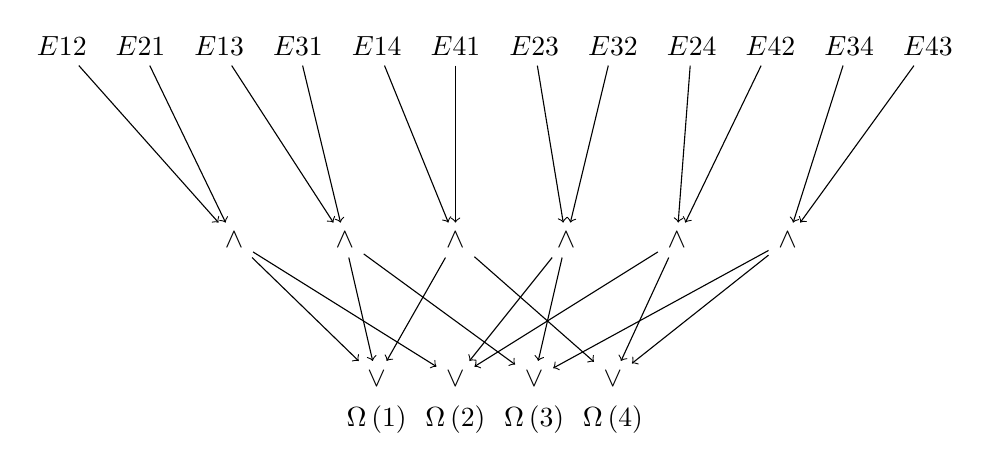
\begin{tikzpicture}

\node (E12) {$E 1 2$};
\node [right of=E12] (E21) {$E 2 1$};
\node [right of=E21] (E13) {$E 1 3$};
\node [right of=E13] (E31) {$E 3 1$};
\node [right of=E31] (E14) {$E 1 4$};
\node [right of=E14] (E41) {$E 4 1$};
\node [right of=E41] (E23) {$E 2 3$};
\node [right of=E23] (E32) {$E 3 2$};
\node [right of=E32] (E24) {$E 2 4$};
\node [right of=E24] (E42) {$E 4 2$};
\node [right of=E42] (E34) {$E 3 4$};
\node [right of=E34] (E43) {$E 4 3$};

\node [below of=E41,node distance=7em] (14) {$\wedge$};
\node [left of=14,node distance=4em] (13) {$\wedge$};
\node [left of=13,node distance=4em] (12) {$\wedge$};
\node [right of=14,node distance=4em] (23) {$\wedge$};
\node [right of=23,node distance=4em] (24) {$\wedge$};
\node [right of=24,node distance=4em] (34) {$\wedge$};

\node [below of=14,node distance=5em,label=below:$\Omega\left(2\right)$] (2) {$\vee$};
\node [left of=2,label=below:$\Omega\left(1\right)$] (1) {$\vee$};
\node [right of=2,label=below:$\Omega\left(3\right)$] (3) {$\vee$};
\node [right of=3,label=below:$\Omega\left(4\right)$] (4) {$\vee$};

\path [->]
		(E12) edge (12) (E21) edge (12)
		(E13) edge (13) (E31) edge (13)
		(E14) edge (14) (E41) edge (14)
		(E23) edge (23) (E32) edge (23)
		(E24) edge (24) (E42) edge (24)
		(E34) edge (34) (E43) edge (34)

		(12) edge (1) (12) edge (2)
		(13) edge (1) (13) edge (3)
		(14) edge (1) (14) edge (4)
		(23) edge (2) (23) edge (3)
		(24) edge (2) (24) edge (4)
		(34) edge (3) (34) edge (4)

;

\end{tikzpicture}
\par\end{centering}

\caption{Schaltkreis $\mathcal{C}_{4}$}


\end{figure}

\end{example*}

\subsection{Eigenschaften von Schaltkreisen}
\begin{defn}
\textbf{Größe und Tiefe}

Die \textbf{Größe} $\left|\mathcal{C}\right|$ eines Schaltkreises
$\mathcal{C}=\left(G,W,\Sigma,\Omega,U\right)$ sei die Anzahl seiner
Gates, $\left|G\right|$.

Die \textbf{Tiefe} $T\left(\mathcal{C}\right)$ sei die maximale Länge
eines einfachen Wegs durch den Graphen $\left(G,W\right)$.
\end{defn}

\begin{defn}
\textbf{Invarianz}

Ein $k$-stelliger $\left(\sigma,\mathbb{B}\right)$-Schaltkreis $\mathcal{C}$
mit dem Universum $U$ heiße \textbf{invariant} wenn für alle $\mathfrak{A}\in\mathbf{FIN}_{<}\left(\sigma\right)$,
alle $\bar{a}\in A^{\mathrm{ar}\left(\mathcal{C}\right)}$ und alle
Bijektionen $\pi_{1},\pi_{2}:A\rightarrow U$ gilt:
\[
q_{\mathcal{C}}\left(\pi_{1}\mathfrak{A}\right)=q_{\mathcal{C}}\left(\pi_{2}\mathfrak{A}\right)
\]


In diesem Fall definieren wir für jede Struktur $\mathfrak{A}\in\mathbf{FIN}^{\left(\left|U\right|\right)}\left(\sigma\right)$
die Auswertung von $\mathcal{C}$ implizit als die Auswertung auf
$\pi\mathfrak{A}\in\mathbf{FIN}^{U}\left(\sigma\right)$ mit einer
beliebigen Bijektion $\pi:A\rightarrow U$:
\[
q_{\mathcal{C}}\left(\mathfrak{A}\right)\coloneqq\pi^{-1}\left(q_{\mathcal{C}}\left(\pi\mathfrak{A}\right)\right)
\]

\end{defn}

\begin{defn}
\textbf{Symmetrie}
\end{defn}
Ein $k$-stelliger Schaltkreis $\mathcal{C}=\left(G,W,\Sigma,\Omega,U\right)$
heiße \textbf{symmetrisch}, wenn jede Permutation der Universums $\pi\in\mathrm{Sym}_{U}$
einen Automorphismus $\hat{\pi}:G\tilde{\rightarrow}G$ des Graphen
$\left(G,W\right)$ induziert, der die folgenden Bedingungen erfüllt:
\begin{enumerate}
\item Für alle Inputs $g$ mit $\Sigma\left(g\right)=R\bar{x}$ gilt $\Sigma\left(\hat{\pi}g\right)=R\,\bar{x'}$,
mit $\bar{x'}=\pi\bar{x}$.
\item Für alle übrigen Gates gilt $\Sigma\left(\hat{\pi}g\right)=\Sigma\left(g\right)$.
\item Für jedes Tupel $\bar{t}\in U^{k}$ gilt $\hat{\pi}\Omega\left(\bar{x}\right)=\Omega\left(\pi\bar{t}\right)$.\end{enumerate}
\begin{prop}
Symmetrie ist eine hinreichende, aber nicht notwendige, Bedingung
für die Invarianz eines Schaltkreises.\end{prop}
\begin{proof}
Sei $\mathcal{C}$ ein symmetrischer $k$-stelliger $\left(\sigma,\mathbb{B}\right)$-Schaltkreis
über $U$, und $\mathfrak{A}\in\mathbf{FIN}^{\left(\left|U\right|\right)}\left(\sigma\right)$.
Seien $\pi_{1},\pi_{2}:A\rightarrow U$ zwei beliebige Bijektionen,
und sei $\bar{a}\in A^{k}$ ein beliebiges Tupel. Es ist zu zeigen,
dass: 
\begin{eqnarray*}
\mathcal{C}\left[\pi_{1}\mathfrak{A}\right]\left(\Omega\left(\pi_{1}\bar{a}\right)\right) & = & \mathcal{C}\left[\pi_{2}\mathfrak{A}\right]\left(\Omega\left(\pi_{2}\bar{a}\right)\right)
\end{eqnarray*}


Wir definieren die Permutation $\tau\in\mathrm{Sym}_{U}$ als $\tau\coloneqq\pi_{1}\pi_{2}^{-1}$,
so dass $\pi_{1}=\tau\pi_{2}$.

Wegen der Symmetrie induziert $\tau$ einen Automorphismus $\hat{\tau}$
auf $\mathcal{C}$: 
\begin{eqnarray*}
\hat{\tau}\left(W\right) & = & W\\
\Sigma\left(\hat{\tau}g\right) & = & \begin{cases}
R\tau\bar{x} & \mathrm{f\ddot{u}r}\,\,\Sigma\left(g\right)=R\bar{x}\\
\Sigma\left(g\right) & \mathrm{sonst}
\end{cases}\\
\Omega\left(\tau\bar{x}\right) & = & \hat{\tau}\Omega\left(\bar{x}\right)\,\mathrm{f\ddot{u}r\,alle}\,\bar{x}\in U^{\mathrm{ar}\left(\mathcal{C}\right)}
\end{eqnarray*}


Per Induktion über die Tiefe $T\left(g\right)$ des Gates $g$\footnote{Die Tiefe $T:G\rightarrow\mathbb{N}$ sei die maximale Länge eines
Weges von einer Quelle zum Gate $g$.} wird gezeigt: 
\begin{eqnarray*}
\mathcal{C}\left[\tau\pi_{2}\mathfrak{A}\right]\left(\hat{\tau}g\right)=\mathcal{C}\left[\pi_{2}\mathfrak{A}\right]\left(g\right) &  & \mathrm{f\ddot{u}r\,alle}\,g\in G
\end{eqnarray*}

\begin{description}
\item [{Induktionsanfang~$T\left(g\right)=0$:}] Sei $g\in G$ ein Input
mit $\Sigma\left(g\right)=R\bar{x}$. Per Definition von $\tau$ und
$\hat{\tau}$ gilt:
\begin{eqnarray*}
\Sigma\left(\hat{\tau}g\right) & = & R\tau\bar{x}\\
\tau\bar{x}\in\tau\pi_{2}R^{\mathfrak{A}} & \Longleftrightarrow & \bar{x}\in\pi_{2}R^{\mathfrak{A}}
\end{eqnarray*}
 Es folgt: 
\begin{eqnarray*}
\mathcal{C}\left[\tau\pi_{2}\mathfrak{A}\right]\left(\hat{\tau}g\right) & = & \left[\tau\pi_{2}R^{\mathfrak{A}}\right]\left(\tau\bar{x}\right)\\
 & = & \left[\pi_{2}R^{\mathfrak{A}}\right]\left(\bar{x}\right)\\
 & = & \mathcal{C}\left[\pi_{2}\mathfrak{A}\right]\left(g\right)
\end{eqnarray*}
(Falls $\Sigma\left(g\right)\in\left\{ \mathbf{0},\mathbf{1}\right\} $,
folgt die Behauptung direkt aus $\Sigma\left(\hat{\tau}g\right)=\Sigma\left(g\right)$.)
\item [{Induktionsschritt~$n\mapsto n+1$:}]~

\begin{description}
\item [{Annahme:}] Für alle Gates $g\in G$ mit Tiefe $T\left(g\right)\leqslant n$
gilt $\mathcal{C}\left[\tau\pi_{2}\mathfrak{A}\right]\left(\hat{\tau}g\right)=\mathcal{C}\left[\pi_{2}\mathfrak{A}\right]\left(g\right)$.
\end{description}

So gilt für jedes Gatter $g'\in G$ mit $T\left(g'\right)=n+1$: 
\begin{enumerate}
\item Die Beschriftungen $\Sigma\left(\hat{\tau}g'\right)=\Sigma\left(g'\right)=\phi$
sind gleich.
\item $\mathcal{C}\left[\tau\pi_{2}\mathfrak{A}\right]\left(\hat{\tau}g\right)=\mathcal{C}\left[\pi_{2}\mathfrak{A}\right]\left(g\right)$
für alle $\left(g,g'\right)\in W$.
\end{enumerate}

Es folgt $\mathcal{C}\left[\tau\pi_{2}\mathfrak{A}\right]\left(\hat{\tau}g'\right)=\mathcal{C}\left[\pi_{2}\mathfrak{A}\right]\left(g'\right)$.

\end{description}
Schließlich gilt für jedes Tupel $\bar{a}\in A^{\mathrm{ar}\left(\mathcal{C}\right)}$:

\begin{eqnarray*}
\mathcal{C}\left[\pi_{1}\mathfrak{A}\right]\left(\Omega\left(\pi_{1}\bar{a}\right)\right) & = & \mathcal{C}\left[\tau\pi_{2}\mathfrak{A}\right]\left(\Omega\left(\tau\pi_{2}\bar{a}\right)\right)\\
 & = & \mathcal{C}\left[\tau\pi_{2}\mathfrak{A}\right]\left(\hat{\tau}\Omega\left(\pi_{2}\bar{a}\right)\right)\\
 & = & \mathcal{C}\left[\pi_{2}\mathfrak{A}\right]\left(\Omega\left(\pi_{2}\bar{a}\right)\right)
\end{eqnarray*}


Damit ist der Schaltkreis invariant.
\end{proof}

\begin{proof}
Als Gegenbeispiel wird der folgende $0$-stellige Schaltkreis $\mathcal{C}$
über $U=\left\{ 1,2\right\} $ angeführt:

\begin{figure}[H]
\begin{centering}
\begin{center}
\tikzstyle{every node}=[circle, draw=black]
\begin{tikzpicture}

\node [label=below:$\Omega$] (C) {$\wedge$};

\node [above left of=C,node distance=6em] (B1) {$\wedge$};


\node [above left of=B1,node distance=6em] (A1) {$E12$};
\node [right of=A1,node distance=5.5em] (A2) {$E11$};
\node [right of=B1,node distance=5.5em] (A3) {$E22$};
\node [right of=A3,node distance=5.5em] (A4) {$E21$};

\path [->] (A1) edge (B1) (A2) edge (B1) (A3) edge (C) (A4) edge (C)
			(B1) edge (C);
\end{tikzpicture}
\par\end{center}
\par\end{centering}

\caption{Schaltkreis}
\end{figure}

\end{proof}
Der Schaltkreis ist invariant, und akzeptiert alle vollständigen $K_{2}$-Graphen.
Er ist aber nicht symmetrisch: Die Permutation $\left(\begin{array}{cc}
1 & 2\\
2 & 1
\end{array}\right)$ induziert keinen Automorphismus.


\subsection{Eigenschaften von Schaltkreisfamilien}
\begin{defn}
Eine $\left(\sigma,\mathbb{B}\right)$-\textbf{Schaltkreisfamilie}
$\bar{\mathcal{C}}=\left(\mathcal{C}_{n}\right)_{n\in\mathbb{N}}$
sei eine Sequenz von invarianten Schaltkreisen $\mathcal{C}_{n}=\left(G_{n},W_{n},\Sigma_{n},\Omega_{n},U_{n}\right)$
mit der gleichen Stelligkeit $\mathrm{ar}\left(\mathcal{C}_{n}\right)=k$
und den Universen $U_{n}=\left[1,n\right]$.

Die von der Schaltkreisfamilie berechnete $\sigma$-Anfrage $q_{\bar{\mathcal{C}}}$
sei wie folgt: 
\[
q_{\bar{\mathcal{C}}}\left(\mathfrak{A}\right)\coloneqq q_{\mathcal{C}_{\left|A\right|}}\left(\mathfrak{A}\right)
\]

\end{defn}

\begin{defn}
$\mathrm{SBC}$ und $\mathrm{SBC+\mathbf{MAJ}}$\end{defn}
\begin{itemize}
\item Sei $\mathrm{SBC}$ die Klasse aller \textbf{symmetrischen $\left(\sigma,\mathbb{B}_{\mathrm{std}}\right)$-Schaltkreisfamilien}.
\item Sei $\mathrm{SBC}+\mathbf{MAJ}$ die Klasse aller \textbf{symmetrischen
$\left(\sigma,\mathbb{B}_{\mathrm{maj}}\right)$-Schaltkreisfamilien}.
(Zur Erinnerung: $\mathbb{B}_{\mathrm{maj}}=\mathbb{B}_{\mathrm{std}}\uplus\left\{ \mathtt{MAJ}\right\} $,
wobei $\mathtt{MAJ}$ der Majority-Operator ist.)
\end{itemize}

\begin{defn}
\textbf{Uniformität}

Für eine Zeitfunktion $T:\mathbb{N}\rightarrow\mathbb{N}$ sei eine
Schaltkreisfamilie $\bar{\mathcal{C}}$ $T$-\textbf{uniform}, wenn
ein $n_{0}\in\mathbb{N}$ existiert, so dass eine deterministische
Turingmaschine bei Eingabe einer Zahl $n\geqslant n_{0}$ eine Repräsentation
von $\mathcal{C}_{n}$ in höchstens $T\left(n\right)$ Schritten berechnen
kann.

Für eine Klasse von Zeitfunktionen $\mathscr{F}\subseteq\mathrm{Abb}\left(\mathbb{N},\mathbb{N}\right)$
sei sie $\mathscr{F}$-uniform, wenn ein $T\in\mathscr{F}$ existiert,
so dass sie $T$-uniform ist. Insbesondere sei $\mathrm{poly}\left(n\right)$
die Klasse aller polynomiell wachsenden Funktionen, und eine $\mathrm{poly}\left(n\right)$-uniforme
Schaltkreisfamilie heiße ,,P-uniform``.
\end{defn}

\begin{defn}
\textbf{Beschränkte Größe}

Für eine Funktion $f:\mathbb{N}\rightarrow\mathbb{N}$ habe eine Schaltkreisfamilie
$\bar{\mathcal{C}}$ $f$-\textbf{Größe}, wenn für ein $n_{0}\in\mathbb{N}$
und alle $n\geqslant n_{0}$ gilt, dass $\left|\mathcal{C}_{n}\right|\leqslant f\left(n\right)$.
Der Begriff ,,$\mathscr{F}$-groß`` sei analog zu ,,$\mathscr{F}$-uniform``
definiert.\end{defn}
\begin{rem*}
Statt ,,$\mathrm{poly}\left(n\right)$-groß`` wird auch der Begriff
,,$\mathrm{P}/\mathrm{poly}$-uniform`` verwendet:

Eine $\mathrm{P/poly}$-Turingmaschine arbeitet mit einem polynomiell
beschränktem Orakel in Polynomialzeit. Sie kann daher genau solche
Schaltkreisfamilien berechnen, deren binäre Repräsentation polynomielle
Größe hat. Unter Voraussetzung einer geeigneten Kodierung sind dies
genau die $\mathrm{poly}\left(n\right)$-großen Schaltkreisfamilien.\cite{arora-barak}\end{rem*}
\begin{defn}
\textbf{Beschränkte Tiefe}

Für eine Funktion $f:\mathbb{N}\rightarrow\mathbb{N}$ habe eine Schaltkreisfamilie
$\bar{\mathcal{C}}$ $f$-\textbf{Tiefe}, wenn $T\left(\mathcal{C}_{n}\right)\leqslant f\left(n\right)$
für ein $n_{0}\in\mathbb{N}$ und alle $n\geqslant n_{0}$. Der Begriff
,,$\mathscr{F}$-tief`` sei analog zu ,,$\mathscr{F}$-groß``
definiert.\end{defn}
\begin{rem*}
$\mathrm{AC}^{0}$ ist die Klasse der $\mathcal{O}\left(1\right)$-tiefen,
$\mathrm{poly}\left(n\right)$-großen Schaltkreisfamilien.
\end{rem*}
\pagebreak{}


\section{Von Formeln zu Schaltkreisen}


\subsection{Logik erster Stufe}

Die Formeln der Logik erster Stufe sind durch symmetrische, $P$-uniforme
$\mathrm{AC}^{0}$-Schaltkreise berechenbar:
\begin{lem}
\label{lem:FO-Circuit}Jede $\mathrm{FO}\left[\sigma\right]$-Formel
$\varphi$ definiert eine $\sigma$-Anfrage $q$, die von einer symmetrischen,
$P$-uniformen Schaltkreis-Familie $\bar{\mathcal{C}^{\varphi}}$
mit $3\left\Vert \varphi\right\Vert $-Tiefe und $5\left\Vert \varphi\right\Vert n^{\mathtt{MF}\left(\varphi\right)}$-Größe
berechnet wird.\end{lem}
\begin{proof}
Sei $\sigma$ eine relationale Signatur, und sei $\varphi\left(\bar{x}\right)$
eine $k$-stellige $\mathrm{FO}\left[\sigma\right]$-Formel.

Per induktiver Konstruktion über den Aufbau von $\varphi$ wird der
$k$-stellige Schaltkreis $\mathcal{C}_{n}^{\varphi}$ über dem Universum
$U\coloneqq\left[1,n\right]$ definiert, so dass $\left\llbracket \varphi\right\rrbracket \left(\mathfrak{A},\bar{t}\right)\Leftrightarrow\left\llbracket \mathcal{C}_{n}^{\varphi}\right\rrbracket \left(\mathfrak{A},\bar{t}\right)$
für alle $n\in\mathbb{N}$, $\mathfrak{A}\in\mathbf{FIN}^{\left[1,n\right]}\left(\sigma\right)$
und $\bar{t}\in\left[1,n\right]^{k}$ gilt. Die Konstruktion ist in
Polynomialzeit berechenbar. Für eine beliebige Permutation $\pi\in\mathrm{Sym}_{U}$
wird ein Automorphismus $\hat{\pi}$ angegeben, und damit die Symmetrie
nachgewiesen.
\begin{casenv}
\item Falls $\varphi\left(\bar{x}\right)=R\bar{y}$ für $R/m\in\sigma$
und $\bar{y}\in\mathrm{frei}\left(\varphi\right)^{m}$, so besteht
$\mathcal{C}_{n}^{\varphi}$ aus $n^{k}$ Gates.

\begin{description}
\item [{Schaltkreis:}] 
\[
\mathcal{C}_{n}^{\varphi}\coloneqq\left(\left\{ g_{\bar{t}}\mid\bar{t}\in U^{k}\right\} ,\emptyset,\Sigma,\Omega,U\right)
\]
Für jedes Tupel $\bar{t}\in U^{k}$ sei $\beta_{\bar{t}}\coloneqq\left(\begin{array}{c}
\bar{x}\\
\bar{t}
\end{array}\right)$ die Belegung der Variablen $\bar{x}$ mit $\bar{t}$:
\begin{eqnarray*}
\Sigma\left(g_{\bar{t}}\right) & \coloneqq & R\beta_{\bar{t}}\left(\bar{y}\right)\\
\Omega\left(\bar{t}\right) & \coloneqq & g_{\bar{t}}
\end{eqnarray*}

\item [{Korrektheit:}] 
\[
\begin{array}{cccccc}
\left\llbracket R\bar{x}\right\rrbracket \left(\mathfrak{A},\bar{t}\right) & = & \left[R^{\mathfrak{A}}\right]\left(\beta_{\bar{t}}\bar{y}\right) & = & \mathcal{C}_{n}^{\varphi}\left[\mathfrak{A}\right]\left(g_{\bar{t}}\right)= & \left\llbracket \mathcal{C}_{n}^{\varphi}\right\rrbracket \left(\mathfrak{A},\bar{t}\right)\end{array}
\]

\item [{Symmetrie:}] Sei $\hat{\pi}g_{\bar{t}}\coloneqq g_{\pi\bar{t}}$
für alle Tupel $\bar{t}\in U^{k}$. Per Definition ist $\pi\beta_{\bar{t}}\left(\bar{y}\right)=\beta_{\pi\bar{t}}\left(\bar{y}\right)$
und daher 
\begin{eqnarray*}
\Sigma\left(\hat{\pi}g_{\bar{t}}\right) & = & \pi\Sigma\left(g_{\bar{t}}\right)\\
\Omega\left(\pi\bar{t}\right) & = & \hat{\pi}\Omega\left(\bar{t}\right)
\end{eqnarray*}

\item [{Größe:}] Der Schaltkreis hat die Tiefe $0$ und die Größe $n^{k}=n^{\mathtt{MF}\left(\varphi\right)}$.
\end{description}
\item Falls $\varphi\left(\bar{x}\right)=y_{1}\dot{=}y_{2}$, so besteht
$\mathcal{C}_{n}^{\varphi}$ aus $n^{k}$ isolierten Gates (hier ist
$k\in\left\{ 1,2\right\} $).

\begin{description}
\item [{Schaltkreis:}] 
\[
\mathcal{C}_{n}^{\varphi}\coloneqq\left(\left\{ g_{\bar{t}}\mid\bar{t}\in U^{k}\right\} ,\emptyset,\Sigma,\Omega,U\right)
\]
Für jedes Tupel $\bar{t}\in U^{k}$ sei $\beta_{\bar{t}}\coloneqq\left(\begin{array}{c}
\bar{x}\\
\bar{t}
\end{array}\right)$ die entsprechende Belegung:
\begin{eqnarray*}
\Sigma\left(g_{\bar{t}}\right) & \coloneqq & \begin{cases}
\mathbf{1} & \mathrm{falls}\,\,\beta\left(y_{1}\right)=\beta\left(y_{2}\right)\\
\mathbf{0} & \mathrm{sonst}
\end{cases}\\
\Omega\left(\bar{t}\right) & \coloneqq & g_{\bar{t}}
\end{eqnarray*}

\item [{Korrektheit:}] 
\begin{eqnarray*}
\left\llbracket y_{1}\dot{=}y_{2}\right\rrbracket \left(\mathfrak{A},\bar{t}\right)=1 & \Leftrightarrow & \left(\beta_{\bar{t}}y_{1}=\beta_{\bar{t}}y_{2}\right)\\
 & \Leftrightarrow & \mathcal{C}_{n}^{\varphi}\left[\mathfrak{A}\right]\left(g_{\bar{t}}\right)=1\\
 & \Leftrightarrow & \left\llbracket \mathcal{C}_{n}^{\varphi}\right\rrbracket \left(\mathfrak{A},\bar{t}\right)=1
\end{eqnarray*}

\item [{Symmetrie:}] Sei $\hat{\pi}\left(g_{\bar{t}}\right)\coloneqq g_{\pi\bar{t}}$.
Es gilt $\beta_{\bar{t}}\left(x\right)=\beta_{\bar{t}}\left(x'\right)$
genau dann wenn $\beta_{\pi\bar{t}}\left(x\right)=\beta_{\pi\bar{t}}\left(x\right)$,
und daher ist $\Sigma\left(\hat{\pi}g_{\bar{t}}\right)=\Sigma\left(g_{\pi\bar{t}}\right)$.
\item [{Größe:}] Der Schaltkreis hat die Tiefe $0$ und die Größe $n^{k}=n^{\mathtt{MF}\left(\varphi\right)}$.
\end{description}
\item Falls $\varphi\left(\bar{x}\right)=\varphi_{1}\left(\bar{y_{1}}\right)\wedge\cdots\wedge\varphi_{m}\left(\bar{y_{m}}\right)$
mit $\mathrm{ar}\left(\varphi_{i}\right)=k_{i}$, so besteht $\mathcal{C}_{n}^{\varphi}$
aus der disjunkten Vereinigung aller $\mathcal{C}_{n}^{\varphi_{i}}$
für $1\leqslant i\leqslant m$ mit der folgenden Erweiterung.

\begin{description}
\item [{Schaltkreis:}] 
\begin{eqnarray*}
\mathcal{C}_{n}^{\varphi_{i}} & = & \left(G_{i},W_{i},\Sigma_{i},\Omega_{i},U\right)\\
\mathcal{C}_{n}^{\varphi} & \coloneqq & \left(G,W,\Sigma,\Omega,U\right)
\end{eqnarray*}
Es werden neue Outputs für jedes $k$-Tupel aus $U$ hinzugefügt:
\begin{eqnarray*}
G & \coloneqq & \biguplus_{i=1}^{m}G_{i}\uplus\left\{ g_{\bar{t}}\mid\bar{t}\in U^{k}\right\} 
\end{eqnarray*}
Die Outputs werden entsprechend mit denen von $\mathcal{C}_{n}^{\varphi_{i}}$
verknüpft, wobei $\rho_{i}:U^{k}\rightarrow U^{k_{i}}$ ein $k$-Tupel
$\bar{t}$ wie folgt auf die in $\varphi_{i}$ frei vorkommenden Variablen
reduziere:
\begin{eqnarray*}
\mathrm{Sei}\,\,\,\bar{j} & \in & \left[1,k\right]^{k_{i}}\\
\mathrm{so}\,\mathrm{dass}\,\,\,\bar{y_{i}} & = & \left(x_{\left(j_{1}\right)},\cdots,x_{\left(j_{k_{i}}\right)}\right)
\end{eqnarray*}
\begin{eqnarray*}
\mathrm{dann}\,\,\,\rho_{i}\left(t_{1},\cdots,t_{k}\right) & \coloneqq & \left(t_{\left(j_{1}\right)},\cdots,t_{\left(j_{k_{i}}\right)}\right)
\end{eqnarray*}
\begin{eqnarray*}
W & \coloneqq & \bigcup_{i=1}^{m}W_{i}\cup W_{\wedge}\\
W_{\wedge} & \coloneqq & \left\{ \left(\Omega_{i}\left(\rho_{i}\bar{t}\right),g_{\bar{t}}\right)\mid1\leqslant i\leqslant m,\,\bar{t}\in U^{k}\right\} 
\end{eqnarray*}
Die Gates werden entsprechend beschriftet:
\begin{eqnarray*}
\Sigma\left(g\right) & \coloneqq & \begin{cases}
\Sigma_{i}\left(g\right) & \mathrm{f\ddot{u}r}\,\,g\in G_{i}\\
\wedge & \mathrm{sonst}
\end{cases}\\
\Omega\left(\bar{t}\right) & \coloneqq & g_{\bar{t}}\,\,\mathrm{f\ddot{u}r\,alle\,\,}\bar{t}\in U^{k}
\end{eqnarray*}

\item [{Korrektheit:}] Es gilt für $\bar{t}\in U^{k}$: 
\begin{eqnarray*}
\left\llbracket \varphi_{1}\wedge\cdots\wedge\varphi_{m}\right\rrbracket \left(\mathfrak{A},\bar{t}\right) & = & \min_{1\leqslant i\leqslant m}\left\llbracket \varphi_{i}\right\rrbracket \left(\mathfrak{A},\bar{t}\right)\\
 & = & \min_{1\leqslant i\leqslant m}\mathcal{C}_{n}^{\varphi_{i}}\left[\mathfrak{A}\right]\left(\Omega_{i}\left(\rho_{i}\bar{t}\right)\right)\\
 & = & \mathcal{C}_{n}^{\varphi}\left[\mathfrak{A}\right]\left(g_{\bar{t}}\right)
\end{eqnarray*}

\item [{Symmetrie:}] Es existieren bereits die Automorphismen $\hat{\pi_{i}}$
für jeden Schaltkreis $\mathcal{C}_{n}^{\varphi_{i}}$. Der Automorphismus
$\hat{\pi}$ erweitert diese wie folgt:
\[
\hat{\pi}\left(g\right)\coloneqq\begin{cases}
\hat{\pi}_{i}\left(g\right) & \mathrm{f\ddot{u}r}\,g\in G_{i}\\
g_{\pi\bar{t}} & \mathrm{f\ddot{u}r}\,g=g_{\bar{t}}
\end{cases}
\]
Für die Gates und Kanten der Schaltkreise $\mathcal{C}_{n}^{\varphi_{i}}$
ist $\hat{\pi}$ per Annahme bereits korrekt.

\begin{enumerate}
\item Für jede neue Kante $\left(\Omega_{i}\left(\rho_{i}\bar{t}\right),g_{\bar{t}}\right)\in W_{\wedge}$
gilt nach Voraussetzung: 
\begin{eqnarray*}
\left(\hat{\pi}\Omega_{i}\left(\rho_{i}\bar{t}\right),\hat{\pi}g_{\bar{t}}\right) & = & \left(\hat{\pi}_{i}\Omega_{i}\left(\rho_{i}\bar{t}\right),\hat{\pi}g_{\bar{t}}\right)\\
 & = & \left(\Omega_{i}\left(\rho_{i}\pi\bar{t}\right),g_{\pi\bar{t}}\right)\\
 & \in & W_{\wedge}
\end{eqnarray*}
(Die Reduktion $\rho_{i}:U^{k}\rightarrow U^{k_{i}}$ ist ein Homomorphismus
und kommutiert mit der Permutation $\pi$.)
\item Es gilt $\Sigma\left(\hat{\pi}g_{\bar{t}}\right)=\Sigma\left(g_{\bar{t}}\right)=\wedge$.
\item Es gilt $\hat{\pi}\Omega\left(\bar{t}\right)=\hat{\pi}g_{\bar{t}}=g_{\pi\bar{t}}=\Omega\left(\pi\bar{t}\right)$.
\end{enumerate}
\item [{Größe:}] Der Schaltkreis hat die Tiefe $T\left(\mathcal{C}_{n}^{\varphi}\right)$
und die Größe $\left|\mathcal{C}_{n}^{\varphi}\right|$: 
\begin{eqnarray*}
T\left(\mathcal{C}_{n}^{\varphi}\right) & = & 1+\max_{i=1}^{m}T\left(\mathcal{C}_{n}^{\psi_{i}}\right)\\
 & \overset{\mathrm{Ann.}}{\leqslant} & 1+3\max_{i=1}^{m}\left\Vert \psi_{i}\right\Vert \\
 & \leqslant & 1+3\sum_{i=1}^{m}\left\Vert \psi_{i}\right\Vert \leqslant3\left\Vert \varphi\right\Vert 
\end{eqnarray*}
 
\begin{eqnarray*}
\left|\mathcal{C}_{n}^{\varphi}\right| & = & n^{k}+\sum_{i=1}^{m}\left|\mathcal{C}_{n}^{\psi_{i}}\right|\\
 & \overset{\mathrm{Ann.}}{\leqslant} & n^{k}+5\sum_{i=1}^{m}\left\Vert \psi_{i}\right\Vert n^{\mathtt{MF}\left(\psi_{i}\right)}\\
 & \leqslant & n^{\mathtt{MF}\left(\varphi\right)}+5\sum_{i=1}^{m}\left\Vert \psi_{i}\right\Vert n^{\mathtt{MF}\left(\varphi\right)}\\
 & \leqslant & 5n^{\mathtt{MF}\left(\varphi\right)}\left(1+\sum_{i=1}^{m}\left\Vert \psi_{i}\right\Vert \right)\leqslant5n^{\mathtt{MF}\left(\varphi\right)}\left\Vert \varphi\right\Vert 
\end{eqnarray*}

\end{description}
\item Falls $\varphi\left(\bar{x}\right)=\varphi_{1}\vee\cdots\vee\varphi_{\ell}$,
so ist der Schaltkreis analog zu Fall 3 mit $\Sigma\left(g_{\bar{t}}\right)=\vee$.
\item Falls $\varphi\left(\bar{x}\right)=\neg\psi$, so wird der Schaltkreis
$\mathcal{C}_{n}^{\psi}$ wie folgt erweitert:

\begin{description}
\item [{Schaltkreis:}] 
\begin{eqnarray*}
\mathcal{C}_{n}^{\psi} & = & \left(G',W',\Sigma',\Omega',U\right)\\
\mathcal{C}_{n}^{\varphi} & \coloneqq & \left(G,W,\Sigma,\Omega,U\right)
\end{eqnarray*}
Für jedes Tupel $\bar{t}\in U^{k}$ wird ein neues Gate $g_{\bar{t}}$
eingefügt. Die Gates werden mit den Outputs von $\mathcal{C}_{n}^{\varphi'}$
verknüpft. 
\begin{eqnarray*}
G & \coloneqq & G'\uplus\left\{ g_{\bar{t}}\mid\bar{t}\in U^{k}\right\} \\
W & \coloneqq & W'\cup W_{\neg}\\
W_{\neg} & \coloneqq & \left\{ \left(\Omega'\left(\bar{t}\right),g_{\bar{t}}\right)\mid\bar{t}\in U^{k}\right\} \\
\Sigma\left(g\right) & \coloneqq & \begin{cases}
\Sigma'\left(g\right) & \mathrm{falls}\,\,g\in G'\\
\neg & \mathrm{sonst}
\end{cases}\\
\Omega\left(\bar{t}\right) & \coloneqq & g_{\bar{t}}
\end{eqnarray*}

\item [{Korrektheit:}] 
\begin{eqnarray*}
\left\llbracket \neg\psi\right\rrbracket \left(\mathfrak{A},\bar{t}\right) & = & 1-\left\llbracket \psi\right\rrbracket \left(\mathfrak{A},\bar{t}\right)\\
 & = & 1-\mathcal{C}_{n}^{\psi}\left[\mathfrak{A}\right]\left(\Omega'\left(\bar{t}\right)\right)\\
 & = & \mathcal{C}_{n}^{\varphi}\left[\mathfrak{A}\right]\left(g_{\bar{t}}\right)
\end{eqnarray*}

\item [{Symmetrie:}] Es existiert bereits der Automorphismus $\hat{\pi'}$.
Dieser wird wie folgt erweitert:
\[
\hat{\pi}\left(g\right)\coloneqq\begin{cases}
\hat{\pi'}\left(g\right) & \mathrm{falls}\,\,g\in G'\\
g_{\pi\bar{t}} & \mathrm{falls}\,\,g=g_{\bar{t}}
\end{cases}
\]
Dann gilt:
\begin{eqnarray*}
\hat{\pi}W_{\neg} & = & \left\{ \left(\hat{\pi}\Omega'\left(\bar{t}\right),\hat{\pi}g_{\bar{t}}\right)\mid\bar{t}\in U^{k}\right\} \\
 & = & \left\{ \left(\Omega'\left(\pi\bar{t}\right),g_{\pi\bar{t}}\right)\mid\bar{t}\in U^{k}\right\} =W_{\neg}\\
\Sigma\left(\hat{\pi}g_{\bar{t}}\right) & = & \Sigma\left(g_{\bar{t}}\right)=\neg
\end{eqnarray*}

\item [{Größe:}] Der Schaltkreis hat die Tiefe $T\left(\mathcal{C}_{n}^{\varphi}\right)$
und die Größe $\left|\mathcal{C}_{n}^{\varphi}\right|$: 
\begin{eqnarray*}
T\left(\mathcal{C}_{n}^{\varphi}\right) & = & 1+T\left(\mathcal{C}_{n}^{\psi}\right)\\
 & \leqslant & 1+3\left\Vert \psi\right\Vert \leqslant3\left\Vert \varphi\right\Vert 
\end{eqnarray*}
\begin{eqnarray*}
\left|\mathcal{C}_{n}^{\varphi}\right| & = & n^{k}+\left|\mathcal{C}_{n}^{\psi}\right|\\
 & \overset{\mathrm{Ann.}}{\leqslant} & n^{k}+5\left\Vert \psi\right\Vert n^{\mathtt{MF}\left(\psi\right)}\\
 & \leqslant & 5n^{\mathtt{MF}\left(\varphi\right)}+5\left\Vert \psi\right\Vert n^{\mathtt{MF}\left(\varphi\right)}\\
 & \leqslant & 5\left\Vert \varphi\right\Vert n^{\mathtt{MF}\left(\varphi\right)}
\end{eqnarray*}

\end{description}
\item Falls $\varphi\left(\bar{x}\right)=\left(\varphi_{1}\rightarrow\varphi_{2}\right)$,
so ist der Schaltkreis $\mathcal{C}_{n}^{\varphi}\coloneqq\mathcal{C}_{n}^{\left(\neg\varphi_{1}\vee\varphi_{2}\right)}$.
\item Falls $\varphi\left(\bar{x}\right)=\left(\varphi_{1}\left(\bar{y_{1}}\right)\leftrightarrow\varphi_{2}\left(\bar{y_{2}}\right)\right)$,
so besteht $\mathcal{C}_{n}^{\varphi}$ aus der disjunkten Vereinigung
von $\mathcal{C}_{n}^{\varphi_{1}}$ und $\mathcal{C}_{n}^{\varphi_{2}}$
mit der folgenden Erweiterung:
\begin{eqnarray*}
\mathcal{C}_{n}^{\varphi} & \coloneqq & \left(G,W,\Sigma,\Omega,U\right)\\
\mathcal{C}_{n}^{\varphi_{i}} & \coloneqq & \left(G_{i},W_{i},\Sigma_{i},\Omega_{i},U\right)
\end{eqnarray*}


\begin{description}
\item [{Schaltkreis:}] Für jedes Tupel $\bar{t}\in U^{m}$ werden fünf
neue Gates eingefügt:
\begin{eqnarray*}
G & \coloneqq & G_{1}\uplus G_{2}\\
 &  & \uplus\left\{ a_{\bar{t}},b_{\bar{t}},c_{\bar{t}},d_{\bar{t}},e_{\bar{t}}\mid\bar{t}\in U^{k}\right\} 
\end{eqnarray*}
Die Gates $a_{\bar{t}}$ und $b_{\bar{t}}$ negieren die Schaltkreise
$\mathcal{C}_{n}^{\varphi_{1}}$ und $\mathcal{C}_{n}^{\varphi_{2}}$.
Die Gates $\bar{c}_{t}$ und $\bar{d_{t}}$ sind Konjunktionen von
$\left(\varphi_{1}\wedge\varphi_{2}\right)$ und $\left(\neg\varphi_{1}\wedge\neg\varphi_{2}\right)$.
Die Gates $e_{\bar{t}}$ sind die Disjunktionen von $c_{\bar{t}}$
und $d_{\bar{t}}$. 
\begin{eqnarray*}
W & \coloneqq & W_{1}\cup W_{2}\cup W_{\neg}\cup W_{\wedge}\cup W_{\vee}\\
W_{\neg} & \coloneqq & \left\{ \left(\Omega_{1}\left(\rho_{1}\bar{t}\right),a_{\rho_{1}\bar{t}}\right),\,\left(\Omega_{2}\left(\rho_{2}\bar{t}\right),b_{\rho_{2}\bar{t}}\right)\mid\bar{t}\in U^{k}\right\} \\
W_{\wedge} & \coloneqq & \left\{ \begin{array}{c}
\left(\Omega_{1}\left(\rho_{1}\bar{t}\right),c_{\bar{t}}\right),\,\left(\Omega_{2}\left(\rho_{2}\bar{t}\right),c_{\bar{t}}\right),\\
\left(a_{\rho_{1}\bar{t}},d_{\bar{t}}\right),\,\left(b_{\rho_{2}\bar{t}},d_{\bar{t}}\right)
\end{array}\mid\bar{t}\in U^{k}\right\} \\
W_{\vee} & \coloneqq & \left\{ \left(c_{\bar{t}},e_{\bar{t}}\right),\,\left(d_{\bar{t}},e_{\bar{t}}\right)\mid\bar{t}\in U^{k}\right\} 
\end{eqnarray*}
(Hierbei seien $\rho_{1}$ und $\rho_{2}$ analog zu Fall 3 definiert.)
\begin{eqnarray*}
\Sigma\left(g\right) & \coloneqq & \begin{cases}
\neg & \mathrm{f\ddot{u}r}\,\,g\in\left\{ a_{\rho_{1}\bar{t}},b_{\rho_{2}\bar{t}}\mid\bar{t}\in U^{k}\right\} \\
\wedge & \mathrm{f\ddot{u}r}\,\,g\in\left\{ c_{\bar{t}},d_{\bar{t}}\mid\bar{t}\in U^{k}\right\} \\
\vee & \mathrm{f\ddot{u}r}\,\,g\in\left\{ e_{\bar{t}}\mid\bar{t}\in U^{k}\right\} \\
\Sigma_{i}\left(g\right) & \mathrm{f\ddot{u}r}\,\,g\in G_{i}
\end{cases}
\end{eqnarray*}
\[
\Omega\left(\bar{t}\right)=e_{\bar{t}}
\]

\item [{Korrektheit:}] 
\begin{eqnarray*}
\left\llbracket \varphi\right\rrbracket \left(\mathfrak{A},\bar{t}\right) & = & \left\llbracket \left(\varphi_{1}\wedge\varphi_{2}\right)\vee\left(\neg\varphi_{1}\wedge\neg\varphi_{2}\right)\right\rrbracket \left(\mathfrak{A},\bar{t}\right)\\
 & = & \max\left(\begin{array}{c}
\min\left(\left\llbracket \varphi_{1}\right\rrbracket \left(\mathfrak{A},\bar{t}\right),\left\llbracket \varphi_{2}\right\rrbracket \left(\mathfrak{A},\bar{t}\right)\right),\\
\min\left(1-\left\llbracket \varphi_{1}\right\rrbracket \left(\mathfrak{A},\bar{t}\right),1-\left\llbracket \varphi_{2}\right\rrbracket \left(\mathfrak{A},\bar{t}\right)\right)
\end{array}\right)\\
 & = & \max\left(\begin{array}{c}
\min\left(\mathcal{C}_{n}^{\varphi}\left[\mathfrak{A}\right]\left(\Omega_{1}\left(\rho_{1}\bar{t}\right)\right),\mathcal{C}_{n}^{\varphi}\left[\mathfrak{A}\right]\left(\Omega_{2}\left(\rho_{2}\bar{t}\right)\right)\right),\\
\min\left(1-\mathcal{C}_{n}^{\varphi}\left[\mathfrak{A}\right]\left(\Omega_{1}\left(\rho_{1}\bar{t}\right)\right),1-\mathcal{C}_{n}^{\varphi}\left[\mathfrak{A}\right]\left(\Omega_{2}\left(\rho_{2}\bar{t}\right)\right)\right)
\end{array}\right)\\
 & = & \max\left(\begin{array}{c}
\mathcal{C}_{n}^{\varphi}\left[\mathfrak{A}\right]\left(c_{t}\right),\\
\min\left(\mathcal{C}_{n}^{\varphi}\left[\mathfrak{A}\right]\left(a_{\rho_{1}\bar{t}}\right),\mathcal{C}_{n}^{\varphi}\left[\mathfrak{A}\right]\left(b_{\rho_{2}\bar{t}}\right)\right)
\end{array}\right)\\
 & = & \max\left(\mathcal{C}_{n}^{\varphi}\left[\mathfrak{A}\right]\left(c_{t}\right),\mathcal{C}_{n}^{\varphi}\left[\mathfrak{A}\right]\left(d_{\bar{t}}\right)\right)\\
 & = & \mathcal{C}_{n}^{\varphi}\left[\mathfrak{A}\right]\left(e_{\bar{t}}\right)
\end{eqnarray*}

\item [{Symmetrie:}] Es existieren per Annahme die Automorphismen $\hat{\pi_{i}}$
für die Schaltkreise $\mathcal{C}_{n}^{\varphi_{i}}$. Diese werden
wie folgt erweitert:
\[
\hat{\pi}\left(g\right)\coloneqq\begin{cases}
\hat{\pi_{i}}\left(g\right) & \mathrm{f\ddot{u}r}\,\,g\in G_{i}\\
g_{\pi\bar{t}} & \mathrm{f\ddot{u}r}\,\,g=g_{\bar{t}}\,\mathrm{und}\,g\in\left\{ a,b,c,d,e\right\} 
\end{cases}
\]

\item [{Größe:}] Der Schaltkreis hat die Tiefe $T\left(\mathcal{C}_{n}^{\varphi}\right)$
und die Größe $\left|\mathcal{C}_{n}^{\varphi}\right|$:
\begin{eqnarray*}
T\left(\mathcal{C}_{n}^{\varphi}\right) & = & 3+T\left(\mathcal{C}_{n}^{\psi}\right)\\
 & \leqslant & 3+3\left\Vert \psi\right\Vert \leqslant3\left\Vert \varphi\right\Vert 
\end{eqnarray*}
\begin{eqnarray*}
\left|\mathcal{C}_{n}^{\varphi}\right| & = & 5n^{k}+\left|\mathcal{C}_{n}^{\psi}\right|\\
 & \overset{\mathrm{Ann.}}{\leqslant} & 5n^{k}+5\left\Vert \psi\right\Vert n^{\mathtt{MF}\left(\psi\right)}\\
 & \leqslant & 5n^{\mathtt{MF}\left(\varphi\right)}+5\left\Vert \psi\right\Vert n^{\mathtt{MF}\left(\varphi\right)}\\
 & \leqslant & 5\left\Vert \varphi\right\Vert n^{\mathtt{MF}\left(\varphi\right)}
\end{eqnarray*}

\end{description}
\item Falls $\varphi\left(\bar{x}\right)=\exists y_{1}\cdots\exists y_{m}\psi\left(z_{1},\cdots,z_{k+m}\right)$,
so wird der Schaltkreis $\mathcal{C}_{n}^{\varphi'}$ wie folgt erweitert:

\begin{description}
\item [{Schaltkreis:}] 
\begin{eqnarray*}
\mathcal{C}_{n}^{\varphi} & \coloneqq & \left(G,W,\Sigma,\Omega,U\right)\\
\mathcal{C}_{n}^{\varphi'} & \coloneqq & \left(G',W',\Sigma',\Omega',U\right)
\end{eqnarray*}
Sei $\rho:U^{k+m}\rightarrow U^{k}$ die Abbildung, die aus $\bar{z}$
die gebundenen Variablen $\bar{y}$ entferne:
\begin{eqnarray*}
\mathrm{Sei}\,\,\,\bar{i} & \in & \left[1,k\right]^{k}\\
\mathrm{so}\,\mathrm{dass}\,\,\,\bar{x} & = & \left(z_{\left(i_{1}\right)},\cdots,z_{\left(i_{k}\right)}\right)\\
\mathrm{dann}\,\,\,\rho\left(t_{1},\cdots,t_{k}\right) & \coloneqq & \left(t_{\left(i_{1}\right)},\cdots,t_{\left(i_{k}\right)}\right)
\end{eqnarray*}

\end{description}

Es werden neue Outputs eingefügt.
\begin{eqnarray*}
G & \coloneqq & G'\uplus\left\{ g_{\bar{t}}\mid\bar{t}\in U^{k}\right\} 
\end{eqnarray*}
Jedes Gate $\Omega'\left(\bar{u}\right)$ mit $\bar{u}\in U^{k+m}$
wird mit dem Gate $g_{\rho\bar{u}}$ verknüpft.
\begin{eqnarray*}
W & \coloneqq & W'\cup W_{\exists}\\
W_{\exists} & \coloneqq & \left\{ \left(\Omega'\left(\bar{u}\right),g_{\rho\bar{u}}\right)\mid\bar{u}\in U^{k+m}\right\} 
\end{eqnarray*}



Die neuen Outputs werden mit $\vee$ markiert.
\begin{eqnarray*}
\Sigma\left(g\right) & \coloneqq & \begin{cases}
\Sigma'\left(g\right) & \mathrm{f\ddot{u}r}\,g\in G'\\
\vee & \mathrm{sonst}
\end{cases}
\end{eqnarray*}
\[
\Omega\left(\bar{t}\right)\coloneqq g_{\bar{t}}
\]

\begin{description}
\item [{Korrektheit:}] Für $\bar{t}\in U^{k}$ gilt: 
\begin{eqnarray*}
\left\llbracket \varphi\right\rrbracket \left(\mathfrak{A},\bar{t}\right) & = & \max_{\begin{subarray}{c}
\bar{u}\in U^{k+m}\\
\rho\bar{u}=\bar{t}
\end{subarray}}\left\llbracket \psi\right\rrbracket \left(\mathfrak{A},\bar{u}\right)=1\\
 & = & \max_{\begin{subarray}{c}
\bar{u}\in U^{k+m}\\
\rho\bar{u}=\bar{t}
\end{subarray}}\left(\mathcal{C}_{n}^{\varphi}\left[\mathfrak{A}\right]\left(\Omega'\left(\bar{u}\right)\right)\right)\\
 & = & \mathcal{C}_{n}^{\varphi}\left[\mathfrak{A}\right]\left(g_{\bar{t}}\right)
\end{eqnarray*}

\item [{Symmetrie:}] Es existiert bereits der Automorphismus $\hat{\pi'}$.
Dieser wird wie folgt erweitert:
\[
\hat{\pi}\left(g\right)\coloneqq\begin{cases}
\hat{\pi'}\left(g\right) & \mathrm{f\ddot{u}r}\,\,g\in G'\\
g_{\pi\bar{t}} & \mathrm{f\ddot{u}r}\,\,g=g_{\bar{t}}
\end{cases}
\]
Auf den Gates von $\mathcal{C}_{n}^{\varphi'}$ ist $\hat{\pi}$ per
Annahme treu zu $\pi$.

\begin{enumerate}
\item Für die neuen Kanten $\left(\Omega'\left(\bar{u}\right),g_{\rho\bar{u}}\right)\in W$
gilt: $\left(\hat{\pi}\Omega'\left(\bar{u}\right),\hat{\pi}g_{\rho\bar{u}}\right)=\left(\Omega'\left(\pi\bar{u}\right),g_{\rho\pi\bar{u}}\right)\in W$.
\item $\hat{\pi}\Sigma\left(g_{\bar{t}}\right)=\Sigma\left(g_{\bar{t}}\right)=\vee$.
\item $\Omega\left(\pi\bar{t}\right)=g_{\pi\bar{t}}=\hat{\pi}g_{\bar{t}}=\hat{\pi}\Omega\left(\bar{t}\right)$.
\end{enumerate}
\item [{Größe:}] Der Schaltkreis hat die Tiefe $T\left(\mathcal{C}_{n}^{\varphi}\right)$
und die Größe $\left|\mathcal{C}_{n}^{\varphi}\right|$:
\begin{eqnarray*}
T\left(\mathcal{C}_{n}^{\varphi}\right) & = & 1+T\left(\mathcal{C}_{n}^{\psi}\right)\\
 & \leqslant & 1+3\left\Vert \psi\right\Vert \leqslant3\left\Vert \varphi\right\Vert 
\end{eqnarray*}
\begin{eqnarray*}
\left|\mathcal{C}_{n}^{\varphi}\right| & = & n^{k}+\left|\mathcal{C}_{n}^{\psi}\right|\\
 & \overset{\mathrm{Ann.}}{\leqslant} & n^{k}+5\left\Vert \psi\right\Vert n^{\mathtt{MF}\left(\psi\right)}\\
 & \leqslant & 5n^{\mathtt{MF}\left(\varphi\right)}+5\left\Vert \psi\right\Vert n^{\mathtt{MF}\left(\varphi\right)}\\
 & \leqslant & 5\left\Vert \varphi\right\Vert n^{\mathtt{MF}\left(\varphi\right)}
\end{eqnarray*}

\end{description}
\item Falls $\varphi\left(\bar{x}\right)=\forall y_{1}\cdots\forall y_{m}\psi\left(\bar{z}\right)$,
so sei der Schaltkreis analog zu Fall 8 mit $\Sigma\left(g_{\bar{t}}\right)\coloneqq\wedge$.
\end{casenv}
\end{proof}
\pagebreak{}


\subsection{Ordnungserweiterung}

Wir betrachten die Logik $\mathrm{FO}+\mathbf{ORD}$, und weisen nach,
dass die Konstruktion aus Lemma \ref{lem:FO-Circuit} angepasst werden
kann, ohne die Klasse der $P$-uniformen symmetrischen $\mathrm{AC}^{0}$-Schaltkreise
zu verlassen.
\begin{lem}
\label{lem:fo-ord}Jede $\left(\mathrm{FO}+\mathbf{ORD}\right)\left[\sigma\right]$-Formel
$\varphi$ definiert eine $\sigma$-Anfrage $q$, die von einer symmetrischen,
$P$-uniformen $\left(\sigma,\mathbb{B}_{\mathrm{std}}\right)$-Schaltkreisfamilie
$\left(\mathcal{C}_{n}\right){}_{n\in\mathbb{N}}$ mit $3\left\Vert \varphi\right\Vert $-Tiefe
und $5\left\Vert \varphi\right\Vert \left(2n+1\right)^{\mathtt{MF}\left(\varphi\right)}$-Größe
berechnet wird.
\end{lem}
(Dieses Lemma bildet die erste Hälfte des Theorems \ref{thm:5.5:fo-ord}.)
\begin{proof}
Sei $\varphi$ eine $k$-stellige $\left(\mathrm{FO}+\mathbf{ORD}\right)\left[\sigma\right]$-Formel.
Für $n\in\mathbb{N}$ und $\mathfrak{A}\in\mathbf{FIN}^{\left(n\right)}\left(\sigma\right)$
wird $\varphi$ auf der disjunkt vereinigten $\left(\sigma\cup\left\{ \leqslant\right\} \right)$-Struktur
$\mathfrak{A}\uplus\Upsilon\left(n\right)$ ausgewertet, wobei $\Upsilon\left(n\right)=\left(\left[0,n\right],\leqslant\right)$
die lineare Ordnung auf $\left[0,n\right]$ ist.

Der Schaltkreis $\mathcal{C}_{n}$ wird aber auf der umbenannten $\sigma$-Struktur
$\mathfrak{A}'\coloneqq\pi\mathfrak{A}\in\mathbf{FIN}^{\left[1,n\right]}\left(\sigma\right)$
mit dem Universum $U=\left[1,n\right]$ ausgewertet.

Vor der Konstruktion muss daher sichergestellt werden, dass das Universum
von $\mathfrak{A}'$ disjunkt von dem Universum der Orakelstruktur
$\Upsilon\left(n\right)$ ist. Dazu wird das Universum $\left[0,n\right]$
von $\Upsilon\left(n\right)$ durch eine Umbenennung nach $\left[n+1,2n+1\right]$
,,verschoben``:
\begin{eqnarray*}
\Upsilon'\left(n\right) & \coloneqq & \rho\Upsilon\left(n\right)\\
\rho & : & \left[0,n\right]\rightarrow\left[n+1,2n+1\right]\\
\rho\left(i\right) & \coloneqq & i+n+1
\end{eqnarray*}


Nun betrachten wir die disjunkte Vereinigung (wobei die Ordnung $\leqslant$
weiterhin nur auf $\left[n+1,2n+1\right]$ definiert ist): 
\[
\mathfrak{A}'\uplus\Upsilon'\left(n\right)\in\mathbf{FIN}^{\left[1,2n+1\right]}\left(\sigma\cup\left\{ \leqslant\right\} \right)
\]


Weil $\Upsilon\left(n\right)\cong\Upsilon'\left(n\right)$ und $\mathfrak{A}\cong\mathfrak{A}'$,
gilt auch $\mathfrak{A}\uplus\Upsilon\left(n\right)\cong\mathfrak{A}'\uplus\Upsilon'\left(n\right)$
(denn der Isomorphismus ist unter disjunkter Vereinigung abgeschlossen):
\[
\left\llbracket \varphi\right\rrbracket \left(\mathfrak{A}\uplus\Upsilon\left(n\right)\right)=\left\llbracket \varphi\right\rrbracket \left(\mathfrak{A}'\uplus\Upsilon'\left(n\right)\right)
\]


Wir konstruieren nun zunächst einen $\left(\sigma\cup\left\{ \leqslant\right\} ,\mathbb{B}_{\mathrm{std}}\right)$-Schaltkreis
$\mathcal{C}_{2n+1}^{\varphi}$ über $U'=\left[1,2n+1\right]$ entsprechend
dem vorhergehenden Beweis für $\mathrm{FO}$. Dieser arbeitet korrekt
auf $\mathfrak{A}'\uplus\Upsilon'\left(n\right)$ und hat offensichtlich
die geforderte Größe $S_{n}\leqslant5\left\Vert \varphi\right\Vert \left(2n+1\right)^{\mathtt{MF}\left(\varphi\right)}$.

Anschließend konstruieren wir daraus den $\left(\sigma,\mathbb{B}_{\mathrm{std}}\right)$-Schaltkreis
\begin{eqnarray*}
\dot{\mathcal{C}_{n}^{\varphi}} & \coloneqq & \left(G,W,\dot{\Sigma},\dot{\Omega},U\right)\\
U & \coloneqq & \left[1,n\right]
\end{eqnarray*}
 indem alle Inputs $\Sigma\left(g\right)=R\bar{t}$ mit $\bar{t}\notin U^{k}$
oder $R\notin\sigma$ durch Konstanten $\dot{\Sigma}\left(g\right)\in\left\{ \mathbf{0},\mathbf{1}\right\} $
ersetzt werden, und die Ausgangsfunktion auf $\dot{\Omega}=\Omega_{\mid U^{k}}$
reduziert wird.
\begin{casenv}
\item Für $\Sigma\left(g\right)=R\bar{t}$ mit $R\in\sigma$ werden die
,,überschüssigen`` Inputs einfach auf $\mathbf{0}$ gesetzt:
\begin{eqnarray*}
\dot{\Sigma}\left(g\right) & \coloneqq & \begin{cases}
R\bar{t} & \mathrm{falls}\,\,\bar{t}\in U^{k}\\
\mathbf{0} & \mathrm{sonst}
\end{cases}
\end{eqnarray*}

\item Für $\Sigma\left(g\right)=t_{1}\dot{\leqslant}t_{2}$ wird das Ordnungsprädikat
fest in den Schaltkreis eingebaut:
\begin{eqnarray*}
\dot{\Sigma}\left(g\right) & \coloneqq & \begin{cases}
\mathbf{1} & \mathrm{falls}\,\,t_{1},t_{2}\in\left[n+1,2n+1\right],\,t_{1}\leqslant t_{2}\\
\mathbf{0} & \mathrm{sonst}
\end{cases}
\end{eqnarray*}

\end{casenv}
Sei nun $\pi\in\mathrm{Sym}_{U}$ eine beliebige Permutation.

Wir betrachten die Erweiterung $\pi'\coloneqq\pi\cup\mathbf{id}_{\mid\left[n+1,2n+1\right]}$,
die die Elemente von $\Upsilon'\left(n\right)$ auf sich selbst abbildet.
Offensichtlich ist $\pi'\in\mathrm{Sym}_{U'}$ eine Permutation von
$U'=\left[1,2n+1\right]$.

Aus der Symmetrie des Schaltkreises $\mathcal{C}_{2n+1}^{\varphi}$
bezüglich $\mathrm{Sym}_{U'}$ (siehe Lemma \ref{lem:FO-Circuit})
folgt die Existenz eines von $\pi'$ induzierten Automorphismus $\hat{\pi}$.

Es wird nun nachgewiesen, dass $\hat{\pi}$ auch ein von $\pi$ induzierter
Automorphismus in $\dot{\mathcal{C}_{n}^{\varphi}}$ ist. Dazu müssen
nur $\dot{\Sigma}$ und $\dot{\Omega}$ betrachtet werden, da der
Graph $\left(G,W\right)$ unverändert bleibt. Ferner betrachten wir
nur die nicht-konstanten Inputs von $\mathcal{C}_{2n+1}^{\varphi}$,
denn ansonsten bleibt $\Sigma$ unverändert.
\begin{casenv}
\item Für $\Sigma\left(g\right)=R\bar{t}$ mit $R\in\sigma$ gilt:

\begin{casenv}
\item Falls $\bar{t}\in U^{k}$:
\[
\dot{\Sigma}\left(\hat{\pi}g\right)=\Sigma\left(\hat{\pi}g\right)=R\pi\bar{t}
\]

\item Sonst:
\[
\dot{\Sigma}\left(\hat{\pi}g\right)=\mathbf{0}=\dot{\Sigma}\left(g\right)
\]

\end{casenv}
\item Für $\Sigma\left(g\right)=t_{1}\dot{\leqslant}t_{2}$ gilt:

\begin{casenv}
\item Falls $t_{1},t_{2}\in\left[n+1,2n+1\right]$ und $t_{1}\leqslant t_{2}$:
\[
\dot{\Sigma}\left(\hat{\pi}g\right)=\mathbf{1}=\dot{\Sigma}\left(g\right)
\]

\item Sonst:
\[
\dot{\Sigma}\left(\hat{\pi}g\right)=\mathbf{0}=\dot{\Sigma}\left(g\right)
\]

\end{casenv}
\end{casenv}
Außerdem gilt ist $U^{k}$ bezüglich $\pi'$ abgeschlossen: 
\[
\hat{\pi}\dot{\Omega}\left(\bar{t}\right)=\hat{\pi}\Omega\left(\bar{t}\right)=\Omega\left(\pi'\bar{t}\right)=\dot{\Omega}\left(\pi'\bar{t}\right)
\]
 Damit ist $\bar{\dot{\mathcal{C}^{\varphi}}}$ eine symmetrische,
$P$-uniforme Schaltkreisfamilie in $\mathrm{AC}^{0}$, die die Anfrage
$q$ berechnet.
\end{proof}
\pagebreak{}


\subsection{Zählquantoren}

Wir betrachten die Logik $\mathrm{FO}+C$, und weisen nach, dass die
vorhergehende Konstruktion aus Lemma \ref{lem:fo-ord} angepasst werden
kann, indem Majority-Gates hinzugefügt werden.
\begin{lem}
\label{lem:fo-c}Jede $\left(\mathrm{FO}+\exists^{\geqslant}\right)\left[\sigma\right]$-Formel
$\varphi$ definiert eine $\sigma$-Anfrage $q$, die von einer symmetrischen,
$P$-uniformen $\left(\sigma,\mathbb{B}_{\mathrm{maj}}\right)$-Schaltkreisfamilie
$\left(\mathcal{C}_{n}\right)_{n\in\mathbb{N}}$ mit $3\left\Vert \varphi\right\Vert $-Tiefe
und $5\left\Vert \varphi\right\Vert \cdot\left(2n+1\right)^{\mathtt{MF}\left(\varphi\right)}$-Größe
berechnet wird.
\end{lem}
(Dieses Lemma bildet die erste Hälfte von Theorem \ref{thm:5.6:fo-c}.)
\begin{proof}
Sei $\varphi$ eine $k$-stellige $\left(\mathrm{FO}+\exists^{\geqslant}\right)\left[\sigma\right]$-Formel.
Der $\left(\sigma\cup\left\{ \leqslant\right\} ,\mathbb{B}_{\mathrm{maj}}\right)$-Schaltkreis
$\mathcal{C}_{2n+1}^{\varphi}$ über dem Universum $U'\coloneqq\left[1,2n+1\right]=\left[1,n\right]\uplus\rho\left[0,n\right]$
wird nach dem gleichen Schema wie in Lemma \ref{lem:fo-ord}, wobei
ein neuer Fall hinzukommt.

(Zur Erinnerung: $\rho:\left[0,n\right]\rightarrow\left[n+1,2n+1\right]$
ist die Verschiebung des Universums von $\Upsilon\left(n\right)$.)
\begin{casenv}
\item Falls $\varphi\left(\bar{x}\right)=\exists^{\geqslant x_{i}}y_{j}\psi\left(\bar{y}\right)$,
so sei $\mathcal{C}_{2n+1}^{\psi}$ der $k$-stellige Schaltkreis
für die Formel $\psi$:
\[
\mathcal{C}_{2n+1}^{\psi}=\left(G_{\psi},W_{\psi},\Sigma_{\psi},\Omega_{\psi},U'\right)
\]


\begin{description}
\item [{Schaltkreis:}] 
\begin{eqnarray*}
\mathcal{C}_{2n+1}^{\varphi} & \coloneqq & \left(G,W,\Sigma,\Omega,U'\right)
\end{eqnarray*}
Es wird für jedes Tupel $\bar{t}\in U'^{k}$ ein neuer Output $g_{\bar{t}}$
eingefügt; ferner werden $2n$ Konstanten eingefügt: 
\begin{eqnarray*}
G & = & G_{\psi}\uplus\left\{ g_{\bar{t}}\mid\bar{t}\in U'^{k}\right\} \uplus\left\{ 0_{j},1_{j}\mid1\leqslant j\leqslant n\right\} \\
W & = & W_{\psi}\uplus W_{\mathrm{maj}}\uplus_{\mathrm{pad}}
\end{eqnarray*}
Die neuen Outputs werden mit $\mathtt{MAJ}$ markiert, falls $t_{i}$
(der Wert der Variable $x_{i}$) einer der numerischen Werte (im Bereich
$\rho\left[0,n\right]=\left[n+1,2n+1\right]$) ist, und sonst mit
$\mathbf{0}$. 
\[
\begin{array}{ccc}
\Sigma\left(0_{j}\right)=\mathbf{0}, & \Sigma\left(0_{j}\right)=\mathbf{1}, & \Sigma\left(g_{\bar{t}}\right)=\begin{cases}
\mathtt{MAJ} & \mathrm{falls}\,\,t_{i}\in\rho\left[0,n\right]\\
\mathbf{0} & \mathrm{sonst}
\end{cases}\end{array}
\]
\[
\Omega\left(\bar{t}\right)=g_{\bar{t}}
\]
Seien $\tau_{1},\tau_{2}:U^{k}\rightarrow U^{k-1}$ die folgenden
Abbildungen, die den Wert $t_{i}$ aus $\bar{t}$ beziehungsweise
$u_{j}$ aus $\bar{u}$ entfernen:
\begin{eqnarray*}
\tau_{1}\left(t_{1},\cdots,t_{k}\right) & = & \left(t_{1},\cdots t_{i-1},t_{i+1},\cdots,t_{k}\right)\\
\tau_{2}\left(t_{1},\cdots,t_{k}\right) & = & \left(t_{1},\cdots t_{j-1},t_{j+1},\cdots,t_{k}\right)
\end{eqnarray*}
Es gilt also $\tau_{1}\left(\bar{t}\right)=\tau_{2}\left(\bar{u}\right)$
genau dann wenn $\bar{t}$ und $\bar{u}$ in den gemeinsamen freien
Variablen von $\varphi$ und $\psi$ übereinstimmen. Das Majority-Gate
$g_{\bar{t}}$ soll prüfen, ob $t_{i}\leqslant\rho f\left(\tau_{1}\left(\bar{t}\right)\right)$,
wobei $f:U^{k-1}\rightarrow\left[0,n\right]$ die Anzahl der $\psi$
erfüllenden Belegungen von $y_{j}$ bei der Belegung der übrigen freien
Variablen mit $\tau_{1}\left(\bar{t}\right)$ sei: 
\begin{eqnarray*}
f\left(\bar{t'}\right) & \coloneqq & \left|\left\{ u_{j}\in\left[1,n\right]\mid\mathrm{es\,existiert\,}\bar{u}\in q_{\mathcal{C}_{2n+1}^{\psi}}\left(\mathfrak{A}\uplus\rho\Upsilon\left(n\right)\right),\,\tau_{2}\left(\bar{u}\right)=\bar{t'}\right\} \right|
\end{eqnarray*}
Dazu wird jedes Gate $g_{\bar{t}}$ mit $t_{i}\in\left[n+1,2n+1\right]$
zunächst mit den entsprechenden Outputs von $\mathcal{C}_{2n+1}^{\psi}$
verknüpft: 
\[
W_{\mathrm{maj}}=\left\{ \left(\Omega_{\psi}\left(\bar{u}\right),g_{\bar{t}}\right)\mid\bar{t},\bar{u}\in U'^{k},\,\tau_{1}\left(\bar{t}\right)=\tau_{2}\left(\bar{u}\right),\,u_{j}\in\left[1,n\right]\right\} 
\]
Momentan hat es genau $n$ Eingänge (für jeden Wert $u_{j}\in\left[1,n\right]$).
Daher gibt es $1$ aus, wenn $f\left(\bar{t}\right)\geqslant\frac{n}{2}$.
Es soll aber berechnen, ob $f\left(\bar{t}\right)\geqslant\rho^{-1}t_{i}$.
Dazu fügen wir die Kanten $W_{\mathrm{pad}}$ ein, um die Eingänge
der Majority-Gates mit Konstanten aufzufüllen. Ein Majority-Gate mit
$k$ zusätzlichen $\mathbf{0}$-Eingängen entscheidet $f\left(\bar{t}\right)\geqslant\frac{n+k}{2}$,
eines mit $k'$ zusätzlichen $\mathbf{1}$-Eingängen berechnet $f\left(\bar{t}\right)\geqslant\frac{n-k'}{2}$.
Es folgt:
\begin{eqnarray*}
\rho^{-1}t_{i} & \in & \left\{ \frac{n+k}{2},\frac{n-k'}{2}\right\} \\
k=2\rho^{-1}t_{i}-n & \mbox{oder} & k'=n-2\rho^{-1}t_{i}
\end{eqnarray*}
Jedes Majority-Gate $g_{\bar{t}}$ muss entweder $k=2\rho^{-1}t_{i}-n$
$\mathbf{0}$-Eingänge oder $k'=n-2\rho^{-1}t_{i}$ $\mathbf{1}$-Eingänge
erhalten:
\begin{eqnarray*}
W_{\mathrm{pad}} & = & \left\{ \left(0_{j},g_{\bar{t}}\right)\mid\bar{t}\in U'^{k},\,t_{i}\in\rho\left[0,n\right],\,1\leqslant j\leqslant2\rho^{-1}t_{i}-n\right\} \\
 & \cup & \left\{ \left(1_{j},g_{\bar{t}}\right)\mid\bar{t}\in U'^{k},\,t_{i}\in\rho\left[0,n\right],\,1\leqslant j\leqslant n-2\rho^{-1}t_{i}\right\} 
\end{eqnarray*}
\begin{eqnarray*}
\overset{n+k=2\rho^{-1}t_{i}}{\overbrace{x_{1}\cdots x_{n}\underset{k=2\rho^{-1}t_{i}-n}{\underbrace{\mathbf{0}\mathbf{0}\cdots\mathbf{0}}}}} &  & \overset{n+k'=2n-2\rho^{-1}t_{i}}{\overbrace{x_{1}\cdots x_{n}\underset{k'=n-2\rho^{-1}t_{i}}{\underbrace{\mathbf{1}\mathbf{1}\cdots\mathbf{1}}}}}
\end{eqnarray*}

\item [{Symmetrie:}] Der neue Schaltkreis ist offensichtlich nicht symmetrisch
bezüglich $\mathrm{Sym}_{U'}$, denn die Anzahl der konstanten Vorgänger
von $g_{\bar{t}}$ hängt von dem Wert $t_{i}$ ab. Allerdings ist
er symmetrisch bezüglich der Permutationen, die die Werte in $\left[n+1,2n+1\right]$
fixieren. (Da die Induktion in Lemma \ref{lem:FO-Circuit} für eine
beliebige Permutation $\pi$ gilt, funktioniert sie auch für diesen
Spezialfall.)


Sei $\pi\in\mathrm{Sym}_{U}$ beliebig, und $\pi'\coloneqq\pi\cup\mathbf{id}_{\left[n+1,2n+1\right]}$
deren Erweiterung auf $U'$. Nun erweitern wir den Automorphismus
$\hat{\pi}$ von $\mathcal{C}_{2n+1}^{\psi}$ wie folgt: 
\begin{eqnarray*}
\hat{\pi}\left(0_{i}\right) & \coloneqq & 0_{i}\\
\hat{\pi}\left(1_{i}\right) & \coloneqq & 1_{i}\\
\hat{\pi}\left(g_{\bar{t}}\right) & \coloneqq & g_{\pi'\bar{t}}
\end{eqnarray*}

\begin{enumerate}
\item Nun gilt für $W_{\mathrm{maj}}$:
\begin{eqnarray*}
\hat{\pi}W_{\mathrm{maj}} & = & \left\{ \left(\hat{\pi}\Omega_{\psi}\left(\bar{u}\right),\hat{\pi}g_{\bar{t}}\right)\mid\bar{t},\bar{u}\in U'^{k},\,\tau_{1}\left(\bar{t}\right)=\tau_{2}\left(\bar{u}\right),\,u_{j}\in\left[1,n\right]\right\} \\
 & \overset{\mathrm{ind.}}{=} & \left\{ \left(\Omega_{\psi}\left(\pi'\bar{u}\right),\hat{\pi}g_{\bar{t}}\right)\mid\bar{t},\bar{u}\in U'^{k},\,\tau_{1}\left(\bar{t}\right)=\tau_{2}\left(\bar{u}\right),\,u_{j}\in\left[1,n\right]\right\} \\
 & \overset{\mathrm{def.}}{=} & \left\{ \left(\Omega_{\psi}\left(\pi'\bar{u}\right),g_{\pi'\bar{t}}\right)\mid\bar{t},\bar{u}\in U'^{k},\,\tau_{1}\left(\bar{t}\right)=\tau_{2}\left(\bar{u}\right),\,u_{j}\in\left[1,n\right]\right\} 
\end{eqnarray*}
und (weil $\pi'u_{j}\in\left[1,n\right]$ ist, und $\tau_{1},\tau_{2}$
Homomorphismen sind):
\begin{eqnarray*}
 & = & \left\{ \left(\Omega_{\psi}\left(\pi'\bar{u}\right),g_{\pi'\bar{t}}\right)\mid\bar{t},\bar{u}\in U'^{k},\,\tau_{1}\left(\pi'\bar{t}\right)=\tau_{2}\left(\pi\bar{u}\right),\,\pi'u_{j}\in\left[1,n\right]\right\} \\
 & = & W_{\mathrm{maj}}
\end{eqnarray*}

\item Für jede Kante $\left(0_{j},g_{\bar{t}}\right)\in W_{\mathrm{pad}}$
(mit $\bar{t}\in U'^{k}$ und $t_{i}\in\left[n+1,2n+1\right]$, und
$j\in\left[1,2t_{i}-3n-2\right]$):
\begin{eqnarray*}
\left(\hat{\pi}0_{j},\hat{\pi}g_{\bar{t}}\right) & = & \left(0_{j},g_{\pi'\bar{t}}\right)
\end{eqnarray*}
Und weil $\pi't_{i}=t_{i}$, gilt immer noch $j\in\left[1,2\pi't_{i}-3n-2\right]$,
und daher $\left(\hat{\pi}0_{j},\hat{\pi}g_{\bar{t}}\right)\in W_{\mathrm{pad}}$.
Das gleiche gilt analog für die Kanten $\left(\hat{\pi}1_{j},\hat{\pi}g_{\bar{t}}\right)$.
\item Für $\Sigma$:
\begin{eqnarray*}
\Sigma\left(\hat{\pi}0_{j}\right) & = & \Sigma\left(0_{j}\right)\\
\Sigma\left(\hat{\pi}1_{j}\right) & = & \Sigma\left(1_{j}\right)\\
\Sigma\left(\hat{\pi}g_{\bar{t}}\right) & = & \Sigma\left(g_{\pi'\bar{t}}\right)\\
 & = & \begin{cases}
\mathtt{MAJ} & \mathrm{falls}\,\,\pi't_{i}\in\left[n+1,2n+1\right]\\
\mathbf{0} & \mathrm{sonst}
\end{cases}\\
 & = & \Sigma\left(g_{\bar{t}}\right)
\end{eqnarray*}

\item Für $\Omega$ ist $\hat{\pi}\Omega\left(\bar{t}\right)=\hat{\pi}g_{\bar{t}}=g_{\pi'\bar{t}}=\Omega\left(\pi'\bar{t}\right)$
per Definition gegeben.
\end{enumerate}
\item [{Größe:}] 
\begin{eqnarray*}
T\left(\mathcal{C}_{2n+1}^{\varphi}\right) & \leqslant & 1+T\left(\mathcal{C}_{2n+1}^{\psi}\right)\\
 & \overset{\mathrm{Ann.}}{\leqslant} & 1+3\left\Vert \psi\right\Vert \leqslant3\left\Vert \varphi\right\Vert 
\end{eqnarray*}
\begin{eqnarray*}
\left|\mathcal{C}_{2n+1}^{\varphi}\right| & \leqslant & \left(2n+1\right)^{k}+2n+\left|\mathcal{C}_{2n+1}^{\psi}\right|\\
 & \overset{\mathrm{Ann.}}{\leqslant} & \left(2n+1\right)^{k}+2n+5\left\Vert \psi\right\Vert \left(2n+1\right)^{\mathtt{MF}\left(\psi\right)}\\
 &  & 5\left(2n+1\right)^{\mathtt{MF}\left(\varphi\right)}+5\left\Vert \psi\right\Vert \left(2n+1\right)^{\mathtt{MF}\left(\varphi\right)}\\
 & \leqslant & 5\left\Vert \varphi\right\Vert \left(2n+1\right)^{\mathtt{MF}\left(\varphi\right)}
\end{eqnarray*}

\end{description}
\end{casenv}
Nach der Erzeugung von $\mathcal{C}_{2n+1}^{\varphi}$ wird der Schaltkreis
auf die bereits beschriebene Weise zu $\dot{\mathcal{C}_{n}^{\varphi}}$
umgewandelt, in dem die nicht-konstanten Inputs mit Elementen aus
$\left[n+1,2n+1\right]$ zu Konstanten werden. Der neue Schritt fügt
keine nicht-konstanten Inputs hinzu, so dass sich hierbei nichts ändert.

Da der Schaltkreis $\mathcal{C}_{2n+1}^{\varphi}$ für jede Permutation
$\pi\uplus\mathbf{id}_{\left[n+1,2n+1\right]}$ mit $\pi\in\mathrm{Sym}_{\left[1,n\right]}$
einen Automorphismus besitzt, ist der Schaltkreis $\dot{\mathcal{C}_{n}^{\varphi}}$
symmetrisch (siehe Lemma \ref{lem:fo-ord}).

\pagebreak{}
\end{proof}

\subsection{Beliebige Orakel}

Wir betrachten die Logik $\mathrm{FO}+\Upsilon$ für beliebige Orakel
$\Upsilon:\mathbb{N}\rightarrow\mathbf{FIN}_{\leqslant}\left(\eta\right)$,
und weisen nach, dass die Konstruktion aus \ref{lem:fo-ord} auf beliebige
Prädikate erweitert werden kann, wobei die $P$-Uniformität aber nicht
die beschränkte Größe geopfert wird.
\begin{lem}
\label{lem:fo-u}Seien $\eta$ und $\sigma$ disjunkte Signaturen
und $\Upsilon\rightarrow\mathbf{FIN}_{\leqslant}\left(\eta\right)$
ein Orakel.

Jede $\left(\mathrm{FO}+\Upsilon\right)\left[\sigma\right]$-Formel
$\varphi$ definiert eine $\sigma$-Anfrage $q$, die von einer symmetrischen
$\left(\sigma,\mathbb{B}_{\mathrm{std}}\right)$-Schaltkreisfamilie
$\left(\mathcal{C}_{n}\right){}_{n\in\mathbb{N}}$ mit konstanter
Tiefe $3\left\Vert \varphi\right\Vert $-Tiefe und polynomieller Größe
$5\left\Vert \varphi\right\Vert \left(2n+1\right)^{\mathtt{M}\left(\varphi\right)}$-Tiefe
berechnet wird.
\end{lem}
(Dieses Lemma bildet die erste Hälfte von \ref{thm:5.7:fo+u}.)
\begin{proof}
Sei $n\in\mathbb{N}$ beliebig und sei $\rho:\left[0,n\right]\rightarrow\left[n+1,2n+1\right]$
wie bisher definiert. Die Struktur $\Upsilon\left(n\right)$ wird
zu 
\[
\Upsilon'\left(n\right)=\rho\Upsilon'\left(n\right)=\left(\left[n+1,2n+1\right],\left(\rho R^{\Upsilon\left(n\right)}\right)_{R\in\eta}\right)
\]


Zunächst wird der $\left(\sigma\cup\eta\cup\left\{ \leqslant\right\} ,\mathbb{B}_{\mathrm{std}}\right)$-Schaltkreis
$\mathcal{C}_{2n+1}^{\varphi}$ wie in Lemma \ref{lem:fo-ord} erzeugt.

Bei der Erzeugung des $\left(\sigma,\mathbb{B}_{\mathrm{std}}\right)$-Schaltkreises
$\dot{\mathcal{C}_{n}^{\varphi}}$ wird nun der folgende Konstruktionsschritt
hinzugefügt:
\begin{casenv}
\item Falls $\Sigma\left(g\right)=R\bar{t}$ mit $R\in\eta$, $\mathrm{ar}\left(R\right)=k$,
und $\bar{t}\in U'^{k}$:
\[
\dot{\Sigma}\left(g\right)=\begin{cases}
\mathbf{1} & \mathrm{falls}\,\,\bar{t}\in R^{\Upsilon'\left(n\right)}\subseteq\left[n+1,2n+1\right]^{k}\\
\mathbf{0} & \mathrm{sonst}
\end{cases}
\]


\begin{description}
\item [{Symmetrie:}] Wenn $\dot{\Sigma}\left(g\right)=\mathbf{1}$, dann
gilt $\bar{t}\in R^{\Upsilon'\left(n\right)}$, und $\pi'\left(\bar{t}\right)=\bar{t}$
(weil $\pi'_{\mid\left[n+1,2n+1\right]}=\mathbf{id}_{\mid\left[n+1,2n+1\right]}$
ist). Daher ist $\Sigma\left(\hat{\pi}g\right)=R\pi'\bar{t}=R\bar{t}$,
und somit gilt auch $\dot{\Sigma}\left(\hat{\pi}g\right)=\mathbf{1}$.
\end{description}
\end{casenv}
Hierbei ist zu beachten, dass die Relation $R^{\Upsilon'\left(n\right)}$
nicht in Polynomialzeit entscheidbar sein muss, und daher die so definierte
Schaltkreisfamilie nicht mehr $P$-uniform ist.

Offensichtlich ist sie jedoch immer noch $\mathrm{poly}\left(n\right)$-groß
und daher auch $P/\mathrm{poly}$-uniform.

\pagebreak{}
\end{proof}

\subsection{Beliebige Orakel mit Zählquantor}

Für eine Orakellogik mit Zählquantor $\mathrm{FO}+\Upsilon+\exists^{\geqslant}$
werden nun die Konstruktionen aller vorhergehender Abschnitte kombiniert.
\begin{lem}
\label{lem:fo-u-c}Seien $\eta$ und $\sigma$ disjunkte Signaturen
und $\Upsilon:\mathbb{N}\rightarrow\mathbf{FIN}_{\leqslant}\left(\eta\right)$
ein Orakel.

Jede $\left(\mathrm{FO}+\Upsilon+\exists^{\geqslant}\right)\left[\sigma\right]$-Formel
$\varphi$ definiert eine $\sigma$-Anfrage $q$, die von einer symmetrischen
$\left(\sigma,\mathbb{B}_{\mathrm{maj}}\right)$-Schaltkreisfamilie
$\left(\mathcal{C}_{n}\right){}_{n\in\mathbb{N}}$ mit $3\left\Vert \varphi\right\Vert $-Tiefe
und $5\left\Vert \varphi\right\Vert \left(2n+1\right)^{\mathtt{M}\left(\varphi\right)+c}$-Größe
für $c\in\mathbb{N}$ berechnet wird.\end{lem}
\begin{proof}
Zunächst wird die Konstruktion aus Lemma \ref{lem:fo-c} und angewendet,
um eine $P/\mathrm{poly}$-uniforme $\left(\sigma,\mathbb{B}_{\mathrm{maj}}\right)$-Schaltkreisfamilie
$\left(\mathcal{C}_{2n+1}^{\varphi}\right)_{n\in\mathbb{N}}$ zu erzeugen,
die bezüglich Permutationen von $\left[1,n\right]$ symmetrisch ist.

Dann werden die Konstruktionen aus Lemma \ref{lem:fo-ord} und Lemma
\ref{lem:fo-u} kombiniert, um daraus eine symmetrische $P/\mathrm{poly}$-uniforme
$\left(\sigma,\mathbb{B}_{\mathrm{maj}}\right)$-Schaltkreisfamilie
$\left(\dot{\mathcal{C}_{n}^{\varphi}}\right)_{n\in\mathbb{N}}$ zu
erzeugen.
\end{proof}
\pagebreak{}


\subsection{Fixpunktlogik}

Die Fixpunktlogik $\mathrm{LFP}\left[\sigma\right]$ ist echt ausdrucksstärker
als die Logik $\mathrm{FO}\left[\sigma\right]$. Beispielsweise ist
die Erreichbarkeit über einen Pfad beliebiger Länge nicht erststufig
definierbar \cite{Immerman1982,Libkin2012}. In $\mathrm{LFP}\left[\left\{ E\right\} \right]$
wird diese Klasse durch die folgende Formel definiert:
\[
\varphi\left(u,v\right)\coloneqq\left[\mathrm{lfp}_{R,\left(x,y\right)}\,\left(\exists z\,\left(E\left(x,z\right)\wedge R\left(z,y\right)\right)\vee x=y\right)\right]\left(u,v\right)
\]
 Trotzdem kann jede $\mathrm{LFP}\left[\sigma\right]$-Formel $\varphi$
durch eine Familie von $\mathrm{FO}\left[\sigma\right]$-Formeln $\left(\varphi_{n}\right)_{n\in\mathbb{N}}$
mit einer konstanten Anzahl Variablen definiert werden, so dass $\varphi_{n}$
auf den Strukturen der Größe $n$ äquivalent zu $\varphi$ ist. Dies
ist vergleichbar zum $k$-Variablen-Fragment der infinitären Logik
$L_{\infty\omega}^{k}$, welches die Fixpunktlogik einschließt.\cite{Dawar1995a,Kolaitis1992a}
Hier hat jedoch jede einzelne Formel $\varphi_{n}$ eine endliche
Länge.
\begin{lem}
\label{lem:lfp-inf}Für jede $\mathrm{LFP}\left[\sigma\right]$-Formel
$\varphi$ mit $\left\Vert \varphi\right\Vert =c$ und jedes $n\in\mathbb{N}$
existiert eine $\mathrm{FO}\left[\sigma\right]$-Formel $\hat{\varphi}$
mit $\left|\mathrm{var}\left(\varphi_{n}\right)\right|\leqslant2\left|\mathrm{var}\left(\varphi\right)\right|$,
so dass $\models_{n}\left(\hat{\varphi}\leftrightarrow\varphi\right)$.\end{lem}
\begin{proof}
Sei $\varphi\left(\bar{x}\right)$ eine $k$-stellige $\mathrm{LFP}\left[\sigma\right]$-Formel.
Es wird induktiv über den Aufbau von $\varphi$ vorgegangen, wobei
nur der Fall $\varphi=\left[\mathrm{lfp}_{R,\bar{z}}\psi\right]\left(\bar{y}\right)$
nicht-trivial ist.

Falls $\varphi=\left[\mathrm{lfp}_{R,\bar{z}}\psi\right]\left(\bar{y}\right)$
für eine $k$-stellige Relationsvariable $R\in\mathbf{var}_{2}$,
$\bar{z}\in\mathbf{var}^{k}$, eine $\mathrm{LFP}\left[\sigma\cup\left\{ R\right\} \right]$-Formel
$\psi$ und ein $k$-Tupel von $\mathrm{LFP}\left[\sigma\right]$-Termen
$\bar{y}\in\mathbf{var}^{k}$, so existiert per Annahme eine $\mathrm{FO}\left[\sigma\right]$-Formel
$\hat{\psi}$ mit $\models_{n}\left(\hat{\psi}\leftrightarrow\psi\right)$.

Sei $\bar{u}\in\mathbf{var}^{k}\backslash\mathrm{frei}\left(\psi\right)$
ein Tupel von Variablen, die nicht frei in $\hat{\psi}$ vorkommen.
Sei die Sequenz $\left(\psi_{i}\right)_{i\in\mathbb{N}}$ induktiv
wie folgt definiert:
\begin{eqnarray*}
\psi^{0} & \coloneqq & \neg\bar{z}\dot{=}\bar{z}\\
\psi^{i+1} & \coloneqq & \hat{\psi}^{\left(\frac{R\bar{t}}{\chi^{i}\left(\bar{t}\right)}\right)}\\
\chi^{i}\left(\bar{t}\right) & \coloneqq & \exists\bar{u}\left(\bar{t}=\bar{u}\wedge\exists\bar{z}\left(\bar{u}=\bar{z}\wedge\psi^{i}\right)\right)
\end{eqnarray*}
Hierbei sei $\hat{\psi}^{\left(\frac{R\bar{t}}{\chi^{i}\left(\bar{t}\right)}\right)}$
die Formel, die aus $\hat{\psi}$ entsteht, indem jedes Atom $R\bar{t}$
(für irgendein $\bar{t}\in\mathbf{var}^{k}$) durch $\chi^{i}\left(\bar{t}\right)$
ersetzt wird. (Der Zwischenschritt über $\bar{u}$ ist notwendig,
weil $\bar{t}$ und $\bar{z}$ zum Teil die gleichen Variablen enthalten
können, und daher ihr Geltungsbereich nicht überlappen darf.)

Nun gelte:
\[
\hat{\varphi}\coloneqq\exists\bar{z}\left(\bar{x}=\bar{z}\wedge\psi^{n^{k}}\right)
\]

\begin{description}
\item [{Korrektheit:}] Sei $F:2^{A^{k}}\rightarrow2^{A^{k}}$ wie in Definition
\ref{def:lfp} definiert. Außerdem sei $\left(X_{i}\right)_{i\in\mathbb{N}}$
wie folgt: 
\[
X_{i}\coloneqq\left\{ \bar{a}\in A^{k}\mid\mathfrak{A}\models\psi^{i}\left[\bar{a}\right]\right\} 
\]
Wir weisen induktiv nach, dass $X_{i}=F^{i}\left(\emptyset\right)$.

\begin{itemize}
\item $\psi^{0}=\neg\bar{x}\dot{=}\bar{x}$ ist offensichtlich unerfüllbar,
und erkennt daher die Relation $X_{0}=\emptyset=F^{0}\left(\emptyset\right)$.
\item Sei $i\in\mathbb{N}$ beliebig:
\begin{eqnarray*}
\bar{a}\in X_{i+1} & \Leftrightarrow & \mathfrak{A}\models\psi^{i+1}\left[\bar{a}\right]\\
 & \Leftrightarrow & \mathfrak{A}\models\hat{\psi}^{\left(\frac{R\bar{z}}{\chi^{i}\left(\bar{z}\right)}\right)}\left[\bar{a}\right]
\end{eqnarray*}
Per Definition gilt: 
\[
X_{i}\coloneqq\left\{ \bar{a}\mid\mathfrak{A}\models\psi^{i+1}\left[\bar{a}\right]\right\} =\left\{ \bar{a}\mid\mathfrak{A}\models\chi^{i}\left[\bar{a}\right]\right\} 
\]
Und daher:
\begin{eqnarray*}
\bar{a}\in X_{i+1} & \Leftrightarrow & \mathfrak{A}\cup\left(A,\left(\begin{array}{c}
R\\
X_{i}
\end{array}\right)\right)\models\hat{\psi}\left[\bar{a}\right]\\
 & \overset{\mathrm{Ann.}}{\Leftrightarrow} & \mathfrak{A}\cup\left(A,\left(\begin{array}{c}
R\\
F^{i}\left(\emptyset\right)
\end{array}\right)\right)\models\hat{\psi}\left[\bar{a}\right]\\
 & \overset{\mathrm{Def.\ref{def:lfp}}}{\Leftrightarrow} & \bar{a}\in F^{i+1}\left(\emptyset\right)
\end{eqnarray*}

\end{itemize}

Schließlich folgt $X_{n^{k}}=F^{n^{k}}\left(\emptyset\right)=F^{\infty}\left(\emptyset\right)$,
da $\left|F^{\infty}\left(\emptyset\right)\right|\leqslant n^{k}$.
Daher gilt:
\begin{eqnarray*}
\left\llbracket \hat{\varphi}\right\rrbracket \left(\mathfrak{A},\bar{a}\right) & = & \left\llbracket \exists\bar{u}\left(\bar{u}=\bar{y}\wedge\psi^{n^{k}}\right)\right\rrbracket \left(\mathfrak{A},\bar{a}\right)\\
 & = & \left\llbracket R\bar{y}\right\rrbracket \left(\mathfrak{A}\cup\left(A,\left(\begin{array}{c}
R\\
F^{\infty}\left(\emptyset\right)
\end{array}\right)\right),\bar{a}\right)\\
 & \overset{\mathrm{Def.\ref{def:lfp}}}{=} & \left\llbracket \left[\mathrm{lfp}_{R,\bar{z}}\psi\right]\left(\bar{y}\right)\right\rrbracket \left(\mathfrak{A},\bar{a}\right)=\left\llbracket \varphi\right\rrbracket \left(\mathfrak{A},\bar{a}\right)
\end{eqnarray*}


\end{description}
\end{proof}
Leider sind diese Formeln zu \emph{lang}: Wenn das Symbol $R$ mehr
als einmal in $\psi$ vorkommt, ist $\left\Vert \psi_{i+1}\right\Vert \geqslant2\left\Vert \psi_{i}\right\Vert $,
und daher $\left\Vert \varphi\right\Vert \geqslant2^{n^{k}}$ für
$k=\mathrm{ar}\left(R\right)$. Für $\mathcal{C}_{n}^{\varphi}=\mathcal{C}_{n}^{\varphi_{n}}$
könnten wir daher nicht die gewünschte $\mathrm{poly}\left(n\right)$-Größe
ableiten.

Die booleschen Schaltkreise haben jedoch nicht dieselbe Einschränkung
wie $\mathrm{FO}\left[\sigma\right]$: Die Berechnung einer Teilformel
$\psi_{i}\left(\bar{z}\right)$ kann wiederverwendet werden, ohne
den Schaltkreis $\mathcal{C}_{n}^{\psi_{i}}$ zu vervielfältigen.

\pagebreak{}Wir nutzen dies und den Beweis von Lemma \ref{lem:lfp-inf}
aus, um aus der $\mathrm{LFP}\left[\sigma\right]$-Formel $\left[\mathrm{lfp}_{R,\bar{z}}\psi\right]\left(\bar{y}\right)$
direkt einen $\left(\sigma,\mathbb{B}_{\mathrm{std}}\right)$-Schaltkreis
zu erzeugen, der die gewünschte Tiefe und Größe hat:
\begin{lem}
\label{lem:lfp-circ}Für jede $\mathrm{LFP}\left[\sigma\right]$-Formel
$\varphi$ existiert eine $\left(\sigma,\mathbb{B}_{\mathrm{std}}\right)$-Schaltkreisfamilie
$\bar{\mathcal{C}^{\varphi}}$, so dass $q_{\bar{\mathcal{C}^{\varphi}}}\left(\mathfrak{A}\right)=q_{\varphi}\left(\mathfrak{A}\right)$
für alle $\mathfrak{A}\in\mathbf{FIN}\left(\sigma\right)$.\end{lem}
\begin{proof}
Sei $\varphi\left(\bar{x}\right)$ eine $k$-stellige $\mathrm{LFP}\left[\sigma\right]$-Formel.
Sei $n\in\mathbb{N}$ beliebig. Wir erweitern die Konstruktion aus
Lemma \ref{lem:FO-Circuit} um den folgenden Fall:\end{proof}
\begin{casenv}
\item Sei $\varphi\left(\bar{x}\right)=\left[\mathrm{lfp}_{R,\bar{z}}\psi\right]\left(\bar{y}\right)$
für eine $\ell$-stellige Relationsvariable $R/\ell\in\mathbf{var}_{2}$,
eine $m$-stellige $\mathrm{LFP}\left[\sigma\cup\left\{ R\right\} \right]$-Formel
$\psi\left(\bar{w}\right)$ und ein $\ell$-Tupel von $\mathrm{LFP}\left[\sigma\right]$-Termen
$\bar{y}$.


Zur Übersicht:
\begin{eqnarray*}
\bar{x} & = & \mathbf{var}^{k},\,k=\left|\left\{ x_{1},\cdots,x_{k}\right\} \right|\\
\bar{y},\bar{z} & \in & \mathbf{var}^{\ell},\,\ell=\left|\left\{ z_{1},\cdots,z_{\ell}\right\} \right|\geqslant\left|\left\{ y_{1},\cdots,y_{\ell}\right\} \right|\\
\bar{w} & \in & \mathbf{var}^{m},\,m=\left|\left\{ w_{1},\cdots,w_{m}\right\} \right|\\
\left\{ z_{1},\cdots,z_{\ell}\right\}  & \subseteq & \left\{ w_{1},\cdots,w_{m}\right\} 
\end{eqnarray*}



Wir definieren eine $\mathrm{LFP}\left[\sigma\cup\left\{ R_{1},\cdots,R_{\ell}\right\} \right]$-Formel
$\psi'$, wobei jedes Atom der Form $R\bar{t}$ in $\psi$ durch ein
Atom $R_{i}\bar{t}$ ersetzt wird, und jedes Symbol $R_{i}$ nur einmal
in $\psi'$ vorkommt. (Diese Umbenennung ist notwendig, da jedes Atom
$R\bar{t}$ unterschiedliche freie Parameter aus $\bar{x}$ enthalten
kann, und die Abbildung der Variablen $\bar{x}\bar{z}$ auf $\bar{t}$
fest kodiert werden muss.)


Per Annahme existiert ein $k$-stelliger $\left(\sigma\cup\left\{ R_{1},\cdots,R_{\ell}\right\} ,\mathbb{B}_{\mathrm{std}}\right)$-Schaltkreis
$\mathcal{C}_{n}^{\psi'}$, der auf $\mathfrak{A}\in\mathbf{FIN}^{\left(n\right)}\left(\sigma\cup\left\{ R\right\} \right)$
die Anfrage $q_{\mathcal{C}_{n}^{\psi}}\left(\mathfrak{A}\right)=q_{\psi'}\left(\mathfrak{A}\right)$
berechnet.
\[
\mathcal{C}_{n}^{\psi}=\left(G_{\psi},W_{\psi},\Sigma_{\psi},\Omega_{\psi},U\right)
\]
Sei $\bar{z'}\coloneqq\bar{z}\bar{x}$ die Kombination $\bar{z}$
mit den freien Parametern $\bar{x}$. Für jedes Atom $R_{i}\bar{t}$
sei $\rho_{i}:U^{k+m}\rightarrow U^{m}$ wie folgt:
\begin{eqnarray*}
\mathrm{Sei}\,\,\bar{j} & \in & \left[1,k+m\right]^{m}\\
\mathrm{so\,dass}\,\,\left(t_{1},\cdots,t_{m}\right) & = & \left(z'_{\left(j_{1}\right)},\cdots,z'_{\left(j_{m}\right)}\right)\\
\rho_{i}\bar{u} & = & \left(u_{\left(j_{1}\right)},\cdots,u_{\left(j_{m}\right)}\right)
\end{eqnarray*}

\begin{description}
\item [{Schaltkreis:}] Es wird eine Sequenz $\left(\mathcal{D}^{i}\right)_{i\in\mathbb{N}}$
von $k$-stelligen $\left(\sigma,\mathbb{B}_{\mathrm{std}}\right)$-Schaltkreisen
definiert.
\[
\mathcal{D}^{i}\coloneqq\left(G_{i},W_{i},\Sigma_{i},\Omega_{i},U\right)
\]
 Für $i=0$ nehmen wir nur eine $\mathbf{0}$-Konstante:
\begin{eqnarray*}
\mathcal{D}^{0} & \coloneqq & \left(\left\{ g_{0}\right\} ,\emptyset,\Sigma_{0},\Omega_{0},U\right)\\
\Sigma_{0}\left(g_{0}\right)=\mathbf{0} &  & \Omega\left(\bar{t}\right)=g_{0}
\end{eqnarray*}
Für $i\in\mathbb{N}_{\geqslant1}$ fügen wir eine neue Kopie von $\mathcal{C}_{n}^{\psi}$
in $\mathcal{D}^{i}$ ein:
\begin{eqnarray*}
G_{i+1} & \coloneqq & G_{i}\uplus G_{\psi}\\
W_{i+1} & \coloneqq & W_{i}\uplus W_{\psi}\uplus W'
\end{eqnarray*}
$\mathcal{D}^{i}$ verbindet alle mit $R\bar{t}$ markierten Inputs
mit dem Output $\Omega_{i}\left(\bar{t}\right)$, und markiert sie
mit ,,$\wedge$``. (Hier wäre ,,$\vee$`` äquivalent, da jedes
Gate nur einen Vorgänger hat.) 
\[
\Sigma_{i+1}\left(g\right)\coloneqq\begin{cases}
\Sigma_{i}\left(g\right) & \mathrm{falls}\,\,g\in G_{i}\\
\wedge & \mathrm{falls}\,\,g\in G_{\psi},\,\Sigma_{\psi}\left(g\right)=R\bar{t}\\
\Sigma_{\psi}\left(g\right) & \mathrm{sonst}
\end{cases}
\]
\[
W'\coloneqq\left\{ \left(\Omega_{i}\left(\bar{t}\right),g\right)\mid g\in G_{\psi},\,\Sigma_{\psi}\left(g\right)=R\bar{t}\right\} 
\]
Die Outputs von $\mathcal{C}_{n}^{\psi}$ werden zu den Outputs von
$\mathcal{D}^{i+1}$: 
\[
\Omega_{i+1}=\Omega_{\psi}
\]
Schließlich sei $\mathcal{C}_{n}^{\varphi}\coloneqq\mathcal{D}^{n^{k}}$.
\item [{Korrektheit:}] Es wird induktiv bewiesen, dass $\mathcal{D}^{i}$
auf $\mathfrak{A}\in\mathbf{FIN}\left(\sigma\right)$ die $\sigma$-Anfrage
$q_{\mathcal{D}^{i}}\left(\mathfrak{A}\right)=F^{i}\left(\emptyset\right)$
berechnet. Der Beweis funktioniert analog zu dem von Lemma \ref{lem:lfp-inf}:
\[
q_{\mathcal{D}^{0}}\left(\mathfrak{A}\right)=F^{0}\left(\emptyset\right)=\emptyset
\]
\begin{eqnarray*}
q_{\mathcal{D}^{i+1}}\left(\mathfrak{A}\right) & = & q_{\mathcal{C}_{n}^{\psi}}\left(\mathfrak{A}\cup\left(A,\left(\begin{array}{c}
R\\
q_{\mathcal{D}^{i}}\left(\mathfrak{A}\right)
\end{array}\right)\right)\right)\\
 & \overset{\mathrm{Ann.}}{=} & q_{\mathcal{C}_{n}^{\psi}}\left(\mathfrak{A}\cup\left(A,\left(\begin{array}{c}
R\\
F^{i}\left(\emptyset\right)
\end{array}\right)\right)\right)\\
 & = & q_{\psi}\left(\mathfrak{A}\cup\left(A,\left(\begin{array}{c}
R\\
F^{i}\left(\emptyset\right)
\end{array}\right)\right)\right)\\
 & \overset{\mathrm{Def.\ref{def:lfp}}}{=} & F^{i+1}\left(\emptyset\right)
\end{eqnarray*}
Daher berechnet $\mathcal{C}_{n}^{\varphi}=\mathcal{D}^{n^{k}}$ die
Anfrage $q_{\mathcal{C}_{n}^{\varphi}}\left(\mathfrak{A}\right)=F^{n^{k}}\left(\emptyset\right)=F^{\infty}\left(\emptyset\right)$.
\item [{Größe:}] Es wird induktiv bewiesen, dass $T\left(\mathcal{D}^{i}\right)\leqslant3i\left\Vert \psi\right\Vert +i$,
und $\left|\mathcal{D}^{i}\right|\leqslant5n^{\mathtt{MF}\left(\psi\right)}$
\begin{eqnarray*}
T\left(\mathcal{D}^{0}\right) & = & 0\\
T\left(\mathcal{D}^{i+1}\right) & = & T\left(\mathcal{D}^{i}\right)+T\left(\mathcal{C}_{n}^{\psi}\right)+1\\
 & \leqslant & T\left(\mathcal{D}^{i}\right)+3\left\Vert \psi\right\Vert +1\\
 & \overset{\mathrm{Ann.}}{=} & 3i\left\Vert \psi\right\Vert +i+3\left\Vert \psi\right\Vert +1\\
 & = & 3\left(i+1\right)\left\Vert \psi\right\Vert +i+1
\end{eqnarray*}

\end{description}
\end{casenv}
Mit den bereits beschriebenen Konstruktionen kann aus diesen Formeln
eine Schaltkreisfamilie erzeugt werden, die $\varphi$ berechnet.
\begin{eqnarray*}
\mathcal{C} & \coloneqq & \left(\mathcal{C}_{n}^{\varphi_{n}}\right)_{n\in\mathbb{N}}\\
\mathcal{C}\left(\mathfrak{A}\right) & = & \varphi\left(\mathfrak{A}\right)\,\mathrm{f.a.}\,\mathfrak{A}\in\mathbf{FIN}\left(\sigma\right)
\end{eqnarray*}


Durch die Einschränkung auf eine konstante Anzahl von Variablen ist
die Größe der Schaltkreisfamilie polynomiell durch $n^{\mathcal{O}\left(\left\Vert \varphi\right\Vert \right)}$
beschränkt, obwohl die $\mathrm{FO}\left[\sigma\right]$-Formeln beliebig
lang werden. Die Tiefe ist durch $T\left(\mathcal{C}_{n}^{\varphi_{n}}\right)\in\mathcal{O}\left(\left\Vert \varphi_{n}\right\Vert \right)=\mathcal{O}\left(n^{\left\Vert \varphi\right\Vert }\right)$
allerdings nicht mehr konstant.

Unter der Annahme, dass $\varphi_{n}^{\left(i\right)}\left(\bar{x}\right)$
auf $\mathfrak{A}$ die Anfrage $q\left(\mathfrak{A}\right)=R^{\left(i\right)}$
definiert, definiert $\chi^{\left(n\right)}\left(\bar{z}\right)$
die gleiche Anfrage (mit Umbenennung von $\bar{x}$ in $\bar{z}$).

Daher gilt $\bar{t}\models\left\llbracket \varphi_{n}^{\left(i+1\right)}\left(\bar{x}\right)\right\rrbracket \left(\mathfrak{A}\right)$
genau dann wenn $\bar{t}\models\left\llbracket \psi_{n}\right\rrbracket \left(\mathfrak{A},R^{\left(i\right)}\right)$,
und $\varphi_{n}^{\left(i+1\right)}$ definiert die Anfrage $q\left(\mathfrak{A}\right)=R^{\left(i+1\right)}$.

Schließlich entsteht $\varphi_{n}\left(\bar{y}\right)$ aus $\varphi_{n}^{\left(n^{m}\right)}\left(\bar{x}\right)$,
indem die freien Variablen $x_{1},\cdots,x_{m}$ in $y_{1},\cdots,y_{m}$
umbenannt werden. Damit gilt $\varphi_{n}\equiv_{n}\varphi$.
\begin{proof}
Die so erzeugte Formel $\varphi_{n}$ hat höchstens $\left|\mathrm{var}\left(\varphi\right)\right|+\left\Vert \varphi\right\Vert \leqslant2\left\Vert \varphi\right\Vert $
Variablen: Nur in Fall 4 werden $m$ neue Variablen eingefügt, und
für jeden solchen Induktionsschritt enthält $\varphi$ bereits ein
Tupel $\bar{y}\in\mathbf{var}^{m}$.
\end{proof}
\pagebreak{}


\section{Exkurs in die Gruppentheorie}

Es werden nun mehrere Begriffe eingeführt, mit deren Hilfe wir eine
symmetrische Schaltkreisfamilie logisch beschreiben werden.


\subsection{Partitionen}

Sei $U$ ein beliebiges Universum.
\begin{defn}
Eine \textbf{Partition} $\mathcal{P}$ von $U$ sei eine Menge $\mathcal{P}=\left\{ P_{1},\cdots,P_{k}\right\} $
von disjunkten nicht-leeren Teilmengen $P_{i}\subseteq U$, so dass
$U=\biguplus_{i=1}^{k}P_{i}$. Die Menge aller Partitionen von $U$
sei $\mathrm{Part}_{U}$.

Die Partition $\mathcal{P}$ induziert eine Äquivalenzrelation $\sim_{\mathcal{P}}$
auf $U$, wobei $x\sim_{\mathcal{P}}y$ genau dann wenn $\left\{ x,y\right\} \subseteq P$
für irgendein $P\in\mathcal{P}$.

Die Permutationen aus $\mathrm{Sym}_{U}$ werden auf natürliche Weise
auf $\mathcal{P}$ erweitert. $\pi\mathcal{P}$ ist ebenfalls eine
Partition von $U$:
\begin{eqnarray*}
\pi\mathcal{P} & \coloneqq & \left\{ \pi P_{i}\mid P_{i}\in\mathcal{P}\right\} \\
 & \coloneqq & \left\{ \left\{ \pi x\mid x\in P_{i}\right\} \mid P_{i}\in\mathcal{P}\right\} 
\end{eqnarray*}

\end{defn}

\begin{defn}
Die \textbf{Feinheit }der Partitionen von $U$ sei eine Relation $\preceq$,
so dass $\mathcal{P}\preceq\mathcal{P}'$ (,,$\mathcal{P}$ ist feiner
als $\mathcal{P}'$``) genau dann wenn jedes $P_{i}\in\mathcal{P}$
eine Teilmenge eines $P'_{j}\in\mathcal{P}'$ ist.

Die Relation $\preceq$ ist eine Halbordnung: Sie ist offensichtlich
reflexiv, transitiv und anti-symmetrisch.

Daher bilden die Partitionen von $U$ einen vollständigen Verband
bezüglich den Infimum- und Supremum-Operationen $\sqcap$ und $\sqcup$:
\begin{eqnarray*}
\mathcal{A}\sqcap\mathcal{B} & \coloneqq & \max_{\preceq}\left\{ \mathcal{P}\mid\mathcal{P}\preceq\mathcal{A}\,\mathrm{und}\,\mathcal{P}\preceq\mathcal{B}\right\} \\
\mathcal{A}\sqcup\mathcal{B} & \coloneqq & \min_{\preceq}\left\{ \mathcal{P}\mid\mathcal{A}\preceq\mathcal{P}\,\mathrm{und}\,\mathcal{B}\preceq\mathcal{P}\right\} 
\end{eqnarray*}


($\mathcal{A}\sqcap\mathcal{B}$ sei die gröbste feinere Partition
als $\mathcal{A}$ und $\mathcal{B}$, und $\mathcal{A}\sqcup\mathcal{B}$
die feinste gröbere Partition als $\mathcal{A}$ und $\mathcal{B}$.)\end{defn}
\begin{fact}
Es gilt: 
\begin{eqnarray*}
\mathcal{A}\sqcap\mathcal{B} & = & \left\{ A\cap B\mid A\in\mathcal{B},\,B\in\mathcal{B},\,A\cap B\neq\emptyset\right\} \\
\mathcal{A}\sqcup\mathcal{B} & = & \left\{ \left[x\right]_{\hat{\sim}}\mid x\in U\right\} \\
 &  & \mathrm{wobei}\,\hat{\sim}\coloneqq\left(\sim_{\mathcal{A}}\cup\sim_{\mathcal{B}}\right)^{*}
\end{eqnarray*}
 
\begin{enumerate}
\item $\mathcal{A}\sqcap\mathcal{B}$ besteht aus den nicht-leeren Schnittmengen
von allen Elementen von $\mathcal{A}$ und $\mathcal{B}$, so dass
$\sim_{\mathcal{A}\sqcap\mathcal{B}}=\sim_{\mathcal{A}}\cap\sim_{\mathcal{B}}$.
\item $\mathcal{A}\sqcup\mathcal{B}$ besteht aus den Äquivalenzklassen
der transitiven Hülle von $\sim_{\mathcal{A}}$ und $\sim_{\mathcal{B}}$,
so dass $\sim_{\mathcal{A}\sqcup\mathcal{B}}=$$\left(\sim_{\mathcal{A}}\cup\sim_{\mathcal{B}}\right)^{*}$.
\end{enumerate}
\end{fact}
\begin{defn}
Die feinste und gröbste Partition von $U$ seien $\mathcal{P}_{\min}\left(U\right)\coloneqq\left\{ \left\{ u_{1}\right\} ,\cdots,\left\{ u_{n}\right\} \right\} $
und $\mathcal{P}_{\max}\left(U\right)\coloneqq\left\{ U\right\} $.
\end{defn}
\pagebreak{}


\subsection{Stabilisatoren}
\begin{defn}
Sei $x\in U$. Der \textbf{Stabilisator} von $x$ in $U$ sei die
Untergruppe $\mathrm{Stab}_{U}\left(x\right)\subseteq\mathrm{Sym}_{U}$
mit 
\[
\mathrm{Stab}_{U}\left(x\right)\coloneqq\left\{ \pi\in\mathrm{Sym}_{U}\mid\pi x=x\right\} 
\]

\end{defn}

\begin{defn}
Die vorige Definition wird auf Teilmengen von $U$ erweitert. Sei
$X\subseteq U$:
\begin{itemize}
\item Der \textbf{Punktstabilisator }von $X$ in $U$ sei die Untergruppe
$\mathrm{Stab}_{U}\left(X\right)\subseteq\mathrm{Sym}_{U}$ mit
\[
\mathrm{Stab}_{U}\left(X\right)\coloneqq\left\{ \pi\in\mathrm{Sym}_{U}\mid\pi x=x\,\mathrm{f\ddot{u}r}\,\mathrm{alle}\,x\in X\right\} 
\]
Diese Gruppe ist der Schnitt der Stabilisatoren der Elemente von $X$.
\[
\mathrm{Stab}_{U}\left(X\right)=\bigcap_{x\in X}\mathrm{Stab}_{U}\left(x\right)
\]

\item Der \textbf{Mengenstabilisator} von $X$ in $U$ sei die Untergruppe
$\mathrm{Stab}_{U}\left\{ X\right\} \subseteq\mathrm{Sym}_{U}$ mit
\[
\mathrm{Stab}_{U}\left\{ X\right\} \coloneqq\left\{ \pi\in\mathrm{Sym}_{U}\mid\pi X=X\right\} 
\]
Diese Gruppe ist das Erzeugnis der Vereinigung von $\mathrm{Stab}_{U}\left(X\right)$
und $\mathrm{Stab}_{U}\left(U\backslash X\right)$. 
\[
\mathrm{Stab}_{U}\left\{ X\right\} =\left\langle \mathrm{Stab}_{U}\left(X\right)\cup\mathrm{Stab}_{U}\left(U\backslash X\right)\right\rangle 
\]

\end{itemize}
\end{defn}

\begin{defn}
Die vorige Definition wird auf Partitionen $\mathcal{P}$ von $U$
erweitert:
\begin{itemize}
\item Der Punktstabilisator\textbf{ }von $\mathcal{P}$ in $U$ sei die
Untergruppe $\mathrm{Stab}_{U}\left(\mathcal{P}\right)\subseteq\mathrm{Sym}_{U}$
mit
\begin{eqnarray*}
\mathrm{Stab}_{U}\left(\mathcal{P}\right) & \coloneqq & \left\{ \pi\in\mathrm{Sym}_{U}\mid\pi P_{i}=P_{i}\,\mathrm{f\ddot{u}r}\,\mathrm{alle}\,P_{i}\in\mathcal{P}\right\} 
\end{eqnarray*}
Dies ist der Schnitt der Mengenstabilisatoren der Elemente von $\mathcal{P}$:
\[
\mathrm{Stab}_{U}\left(\mathcal{P}\right)=\bigcap_{P_{i}\in\mathcal{P}}\mathrm{Stab}_{U}\left\{ P_{i}\right\} 
\]

\item Der Mengenstabilisator von $\mathcal{P}$ in $U$ sei die Untergruppe
$\mathrm{Stab}_{U}\left\{ \mathcal{P}\right\} \subseteq\mathrm{Sym}_{U}$
mit
\[
\mathrm{Stab}_{U}\left\{ \mathcal{P}\right\} \coloneqq\left\{ \pi\in\mathrm{Sym}_{U}\mid\pi\mathcal{P}=\mathcal{P}\right\} 
\]
Diese Gruppe ist das Erzeugnis der Vereinigung von $\mathrm{Stab}_{U}\left(\mathcal{P}\right)$
mit allen Permutationen von gleich-mächtigen Elementen der Partition.
Sei für $1\leqslant n\leqslant\left|U\right|$ die Menge $\mathcal{P}_{\mid n}\coloneqq\left\{ P_{i}\in\mathcal{P}\mid\#P_{i}=n\right\} $,
dann gilt: 
\[
\mathrm{Stab}_{U}\left\{ \mathcal{P}\right\} =\left\langle \mathrm{Stab}_{U}\left(\mathcal{P}\right)\cup\bigcup_{i=1}^{\left|U\right|}\mathrm{Sym}_{\mathcal{P}_{\mid i}}\right\rangle 
\]

\end{itemize}
\end{defn}

\subsection{Träger}
\begin{defn}
Sei $G\subseteq\mathrm{\mathrm{Sym}}_{U}$ eine Untergruppe und $\mathcal{P}$
eine Partition von $U$. $\mathcal{P}$ ist ein \textbf{Träger} von\textbf{
}$G$ genau dann wenn $\mathrm{Stab}_{U}\left(\mathcal{P}\right)\subseteq G$.\end{defn}
\begin{rem*}
Wenn $G$ von $\mathcal{P}$ getragen wird, so wird $G$ auch von
allen feineren Elementen $\mathcal{P}'\preceq\mathcal{P}$ getragen
(und $\mathcal{P}$ wiederum trägt alle Obergruppen $G'\supseteq G$).
Dies folgt direkt daraus, dass die Grobheit von Partitionen eine Teilmengenbeziehung
ihrer Stabilisatorgruppen induziert:
\[
\mathcal{P}'\preceq\mathcal{P}\,\,\Longrightarrow\,\,\mathrm{Stab}_{U}\left(\mathcal{P}\right)\subseteq\mathrm{Stab}_{U}\left(\mathcal{P}'\right)
\]
\end{rem*}
\begin{lem}
Die Träger-Eigenschaft ist unter den Operationen $\sqcap$ und $\sqcup$
abgeschlossen.\end{lem}
\begin{proof}
Seien $\mathcal{A}$ und $\mathcal{B}$ Träger einer Gruppe $G\subseteq\mathrm{Sym}_{U}$.

Für $\sqcap$ ist der Beweis per $\mathcal{A}\sqcap\mathcal{B}\preceq\mathcal{A},\mathcal{B}$
trivial.

Sei $\mathcal{P}\coloneqq\mathcal{A}\sqcup\mathcal{B}$, und sei $\pi\in\mathrm{Stab}_{U}\left(\mathcal{P}\right)$
beliebig:
\begin{enumerate}
\item Wenn $\mathcal{P}=\left\{ P_{1},\cdots,P_{k}\right\} $, so existiert
eine Folge von Permutationen $\pi_{1}\cdots\pi_{k}=\pi$, so dass
$\pi_{i}$ nur Elemente von $P_{i}$ miteinander vertauscht:
\[
\pi_{i}\left(x\right)=\begin{cases}
y\in P_{i} & \mathrm{f\ddot{u}r}\,x\in P_{i}\\
x & \mathrm{sonst}
\end{cases}
\]

\item Für jedes $\pi_{i}$ existiert eine Folge von Transpositionen $\left(x_{i,1}y_{i,1}\right)\cdots\left(x_{i,m}y_{i,m}\right)=\pi_{i}$.
\[
\pi=\left(x_{1,1}y_{1,1}\right)\cdots\left(x_{k,m_{k}}y_{k,m_{k}}\right)
\]

\item Für jede dieser Transpositionen $\left(xy\right)$ gilt $x,y\in P_{i}$.
Da $P_{i}\in\mathcal{A}\sqcup\mathcal{B}$ eine Äquivalenzklasse der
transitiven Hülle von $\sim\coloneqq\left(\sim_{\mathcal{A}}\cup\sim_{\mathcal{B}}\right)$
ist, existiert eine Folge von $\ell\leqslant\left|U\right|$ Elementen
$\bar{u}\in U^{\ell}$ mit $u_{1}\sim\cdots\sim u_{\ell}$, so dass
$x=u_{1}$ und $y=u_{\ell}$. Es gilt 
\begin{eqnarray*}
\left(xy\right) & = & \left(u_{1}u_{2}\right)\cdots\left(u_{\ell-1}u_{\ell}\right)\left(u_{\ell-1}u_{\ell-2}\right)\cdots\left(u_{2}u_{1}\right)
\end{eqnarray*}

\item Es gilt $u_{j}\sim_{\mathcal{A}}u_{j+1}$ oder $u_{j}\sim_{\mathcal{B}}u_{j+1}$.
Die Transposition $\left(u_{j}u_{j+1}\right)$ ist somit entweder
in $\mathrm{Stab}_{U}\left(\mathcal{A}\right)\subseteq G$ oder $\mathrm{Stab}_{U}\left(\mathcal{B}\right)\subseteq G$
enthalten.
\item Also ist $\pi$ eine Folge von Permutationen in $G$, und es folgt
$\pi\in G$.
\end{enumerate}
\end{proof}
\begin{cor*}
Jede Gruppe $G\subseteq\mathrm{Sym}_{U}$ besitzt eine eindeutigen
gröbsten Träger.\end{cor*}
\begin{proof}
Jede Gruppe wird mindestens von $\mathcal{P}_{\min}\left(U\right)$
mit $\mathrm{Stab}_{U}\left(\mathcal{P}_{\min}\left(U\right)\right)=\left\{ \mathbf{id}\right\} \subseteq G$
getragen.

Angenommen, $\mathcal{P}$ und $\mathcal{P}'$ seien zwei gröbste
Träger von $G$. 

Nun ist $\mathcal{P}\sqcup\mathcal{P}'$ ebenfalls ein Träger von
$G$, und $\mathcal{P},\mathcal{P}'\preceq\mathcal{P}\sqcup\mathcal{P}'$.

Da $\mathcal{P}$ und $\mathcal{P}'$ aber per Definition gröbste
Träger von $G$ sind, muss $\mathcal{P}=\mathcal{P}\sqcup\mathcal{P}'=\mathcal{P}'$
gelten.\end{proof}
\begin{defn}
Für jede Gruppe $G\subseteq\mathrm{Sym}_{U}$ sei $\mathrm{SP}\left(G\right)$
die gröbste tragende Partition von $G$.
\end{defn}
Wir betrachten nun die Konjugationsoperation auf $\mathrm{Sym}_{U}$.
\begin{lem}
Wenn eine Partition $\mathcal{P}$ ein Träger einer Gruppe $G\subseteq\mathrm{Sym}_{U}$
ist, dann ist $\pi\mathcal{P}$ ein Träger von $\pi G\pi^{-1}$ für
alle $\pi\in\mathrm{Sym}_{U}$.\end{lem}
\begin{proof}
Seien $\vartheta\in\mathrm{Stab}_{U}\left(\pi\mathcal{P}\right)$
und $P_{i}\in\mathcal{P}$ beliebig. Nun gilt:
\begin{eqnarray*}
\left(\pi^{-1}\vartheta\pi\right)P_{i} & = & \pi^{-1}\left(\vartheta\left(\pi P_{i}\right)\right)\\
 & = & \pi^{-1}\pi P_{i}\\
 & = & P_{i}
\end{eqnarray*}


Daraus folgt $\left(\pi^{-1}\vartheta\pi\right)\in\mathrm{Stab}_{U}\left(\mathcal{P}\right)\subseteq G$,
und schließlich:
\begin{eqnarray*}
\vartheta & = & \left(\pi\pi^{-1}\right)\vartheta\left(\pi\pi^{-1}\right)\\
 & = & \pi\left(\pi^{-1}\vartheta\pi\right)\pi^{-1}\\
 & \in & \pi G\pi^{-1}
\end{eqnarray*}


Damit trägt $\pi\mathcal{P}$ die konjugierte Gruppe $\pi G\pi^{-1}$.\end{proof}
\begin{cor*}
Für jede Gruppe $G\subseteq\mathrm{Sym}_{U}$ und jede Permutation
$\pi\in\mathrm{Sym}_{U}$ ist $\pi\mathrm{SP}\left(G\right)=\mathrm{SP}\left(\pi G\pi^{-1}\right)$.\end{cor*}
\begin{proof}
Es wurde gezeigt, dass $\pi\mathrm{SP}\left(G\right)$ ein Träger
von $\pi G\pi^{-1}$ ist. Es folgt:
\[
\pi\mathrm{SP}\left(G\right)\preceq\mathrm{SP}\left(\pi G\pi^{-1}\right)
\]


Umgekehrt ist auch $\pi^{-1}\mathrm{SP}\left(\pi G\pi^{-1}\right)$
ein Träger von $\pi^{-1}\pi G\pi\pi^{-1}=G$. Es folgt:
\[
\pi^{-1}\mathrm{SP}\left(\pi G\pi^{-1}\right)\preceq\mathrm{SP}\left(G\right)
\]


Die Relation $\preceq$ bleibt unter Permutation beider Seiten erhalten:
\begin{eqnarray*}
\mathrm{SP}\left(\pi G\pi^{-1}\right) & \preceq & \pi\mathrm{SP}\left(G\right)
\end{eqnarray*}


Daher ist $\pi\mathrm{SP}\left(G\right)=\mathrm{SP}\left(\pi G\pi^{-1}\right)$.\end{proof}
\begin{lem}
Jede Gruppe $G$ ist Obermenge des Punkt- und Teilmenge des Mengenstabilisators
von $\mathrm{SP}\left(G\right)$:
\[
\mathrm{Stab}_{U}\left(\mathrm{SP}\left(G\right)\right)\subseteq G\subseteq\mathrm{Stab}_{U}\left\{ \mathrm{SP}\left(G\right)\right\} 
\]
\end{lem}
\begin{proof}
Per Definition gilt bereits $\mathrm{Stab}_{U}\left(\mathrm{SP}\left(G\right)\right)\subseteq G$.

Sei nun $\pi\in G$ beliebig. Es gilt:
\begin{eqnarray*}
\pi\mathrm{SP}\left(G\right) & = & \mathrm{SP}\left(\pi G\pi^{-1}\right)\\
 & = & \mathrm{SP}\left(G\right)
\end{eqnarray*}


Daher ist $\pi\in\mathrm{Stab}_{U}\left\{ \mathrm{SP}\left(G\right)\right\} $.\end{proof}
\begin{lem}
Für $\epsilon\in\left[0,1\right[$, jedes hinreichend große Universum
$U$ mit $n\coloneqq\left|U\right|\geqslant\exp\frac{4}{\epsilon}$
und jede Partition $\mathcal{P}\in\mathrm{Part}_{U}$ gilt:

Falls der Index des Mengenstabilisators von $\mathcal{P}$ subexponentiell
in $n$ ist: 
\[
s\coloneqq\frac{\left|\mathrm{Sym}_{U}\right|}{\left|\mathrm{Stab}_{U}\left\{ \mathcal{P}\right\} \right|}\leqslant2^{n^{1-\epsilon}}
\]


Dann enthält $\mathcal{P}$ entweder $\mathcal{O}\left(n^{1-\epsilon}\right)$
oder $n-\mathcal{O}\left(n^{1-\epsilon}\right)$ viele Elemente:
\[
\min\left\{ \left|\mathcal{P}\right|,n-\left|\mathcal{P}\right|\right\} \leqslant\frac{8}{\epsilon}\frac{\log s}{\log n}
\]

\end{lem}
Diese Beziehung ist an der Repräsentation des Mengenstabilisators
als 
\[
\mathrm{Stab}_{U}\left\{ \mathcal{P}\right\} =\left\langle \mathrm{Stab}_{U}\left(\mathcal{P}\right)\cup\bigcup_{i=1}^{\left|U\right|}\mathrm{Sym}_{\mathcal{P}_{\mid i}}\right\rangle 
\]
 erkennbar: Damit sein Index klein ist, muss die Gruppe selbst groß
sein, was entweder einen großen Punktstabilisator oder eine große
Anzahl gleich-mächtiger Elemente von $\mathcal{P}$ erfordert.
\begin{proof}
Sei $\epsilon\in\left[0,1\right[$, $n\geqslant\exp\frac{4}{\epsilon}$,
und $U=\left\{ 1,\cdots,n\right\} $. 

Sei $\mathcal{P}\in\mathrm{Part}_{U}$ beliebig mit $k\coloneqq\left|\mathcal{P}\right|$.
\[
n\leqslant s\coloneqq\frac{\left|\mathrm{Sym}_{U}\right|}{\left|\mathrm{Stab}_{U}\left\{ \mathcal{P}\right\} \right|}\leqslant2^{n^{1-\epsilon}}
\]

\begin{enumerate}
\item Die Definition des Mengenstabilisators liefert eine kombinatorische
Schranke für dessen Größe: Jede Permutation $\pi\in\mathrm{Stab}_{U}\left\{ \mathcal{P}\right\} $
besteht aus einer Permutation der $k$ Elemente von $\mathcal{P}$,
und einer Permutation $\pi_{i}\in\mathrm{Sym}_{P}$ für jedes Element
$P\in\mathcal{P}$. 
\[
\left|\mathrm{Stab}_{U}\left\{ \mathcal{P}\right\} \right|\leqslant k!\prod_{P\in\mathcal{P}}\left|P\right|!
\]

\item Seien $P_{1},\cdots,P_{k}\in\mathcal{P}$ die nach aufsteigender Größe
geordneten Elemente von $\mathcal{P}$, und seien $p_{1}\leqslant\cdots\leqslant p_{k}$
ihre Größen ($\sum_{i=1}^{k}p_{i}=n$). 
\[
\left|\mathrm{Stab}_{U}\left\{ P\right\} \right|\leqslant k!\prod_{i=1}^{k}p_{i}!
\]
.
\item Für zwei beliebige $p_{i},p_{j}$ mit $i\leqslant j$ gilt $p_{i}\leqslant p_{j}$
und daher $\frac{p_{j}+1}{p_{i}}\geqslant1$. Es folgt:
\begin{eqnarray*}
\left|\mathrm{Stab}_{U}\left\{ P\right\} \right| & \leqslant & k!\prod_{i=1}^{k}p_{i}!\\
 & = & k!p_{1}!\cdots p_{i}!\cdots p_{j}!\cdots p_{k}!\\
 & \leqslant & \frac{p_{j}+1}{p_{i}}k!p_{1}!\cdots p_{i}!\cdots p_{j}!\cdots p_{k}!\\
 & = & k!p_{1}!\cdots\left(p_{i}-1\right)!\cdots\left(p_{j}+1\right)!\cdots p_{k}!
\end{eqnarray*}

\item Durch wiederholte Anwendung folgt 
\begin{eqnarray*}
\left|\mathrm{Stab}_{U}\left\{ P\right\} \right| & \leqslant & k!\cdot\underset{k-1}{\underbrace{1!\cdots1!}}\cdot\left(n-\left(k-1\right)\right)!\\
 & = & k!\left(n-k+1\right)!
\end{eqnarray*}
.
\item Nun ist $s$ von unten durch einen Binomialkoeffizienten beschränkt:
\begin{eqnarray*}
s\coloneqq\frac{\left|\mathrm{Sym}_{U}\right|}{\left|\mathrm{Stab}_{U}\left\{ \mathcal{P}\right\} \right|} & = & \frac{n!}{\left|\mathrm{Stab}_{U}\left\{ \mathcal{P}\right\} \right|}\\
 & \geqslant & \frac{n!}{k!\left(n+1-k\right)!}\\
 & = & \frac{1}{n+1}\frac{\left(n+1\right)!}{k!\left(n+1-k\right)!}\\
 & = & \frac{1}{n+1}\binom{n+1}{k}\\
 & \geqslant & \frac{1}{n+1}\binom{n}{k}\\
 & = & \frac{1}{n+1}\binom{n}{\min\left\{ n,n-k\right\} }
\end{eqnarray*}

\item Für den Binomialkoeffizienten gibt es auch eine untere Schranke:\marginpar{CITE}
\[
\binom{n}{k}=\frac{n!}{k!\left(n-k\right)!}=\frac{\prod_{i=n-k+1}^{n}i}{\prod_{i=1}^{k}i}=\prod_{i=1}^{k}\frac{n-k+i}{i}
\]
\[
\left(n-k+1\right)>\frac{\left(n-k+2\right)}{2}>\cdots>\frac{n}{k}
\]
 
\[
\binom{n}{k}\geqslant\left(\frac{n}{k}\right)^{k}
\]

\item Daher ist $s$ von unten beschränkt:
\[
s\geqslant\frac{1}{n+1}\left(\frac{n}{k'}\right)^{k'}
\]

\item Es folgt
\begin{eqnarray*}
\log s & \geqslant & k'\left(\log n-\log k'\right)-\log\left(n+1\right)\\
\log s+\log\left(n+1\right) & \geqslant & k'\left(\log n-\log k'\right)
\end{eqnarray*}

\item Weil $s\geqslant n$ und $\log n\geqslant1$, folgt: 
\begin{eqnarray*}
4\log s & = & \log s+3\log s\\
 & \geqslant & \log s+3\log n\\
 & \geqslant & \log s+\log\left(n+1\right)\\
 & \geqslant & k'\left(\log n-\log k'\right)
\end{eqnarray*}

\item Weil $\frac{n}{k'}\geqslant2$, gilt:
\begin{eqnarray*}
4\log s & \geqslant & k'\left(\log n-\log k'\right)\\
 & \geqslant & k'
\end{eqnarray*}

\item Aus der Bedingung $s\leqslant2^{n^{1-\epsilon}}$ folgt:
\begin{eqnarray*}
\log k' & \leqslant & \log\log s+2\\
 & \leqslant & \log\log2^{n^{1-\epsilon}}+2\\
 & = & \log n^{1-\epsilon}+2\\
 & = & \left(1-\epsilon\right)\log n+2
\end{eqnarray*}

\item Schließlich folgt:
\begin{eqnarray*}
4\log s & \geqslant & k'\left(\log n-\log k'\right)\\
 & \geqslant & k'\left(\log n-\left(1-\epsilon\right)\log n-2\right)\\
 & \geqslant & k'\left(\epsilon\log n-2\right)\\
 & \geqslant & k'\frac{\epsilon\log n}{2}\\
\frac{8\log s}{\epsilon\log n} & \geqslant & k'
\end{eqnarray*}

\end{enumerate}
\end{proof}
Eine Partition, die höchstens $\frac{n}{2}$ Teile enthält (und daher
einen kleinen Nebengruppen-Index $\left[\mathrm{Sym}_{U}:\mathrm{Stab}_{U}\left\{ \mathcal{P}\right\} \right]\leqslant2^{n^{1-\epsilon}}$
hat) muss ein sehr großes Element enthalten.
\begin{lem}
Für $\epsilon\in\left[0,1\right[$, jedes hinreichend große Universum
$U$ mit $n\coloneqq\left|U\right|\geqslant\exp\frac{8}{\epsilon^{2}}$
und eine Partition $\mathcal{P}$ mit mit $\left|\mathcal{P}\right|\leqslant\frac{n}{2}$
Elemente gilt:

Falls der Index des Mengenstabilisators von $\mathcal{P}$ subexponentiell
in $n$ ist: 
\[
s\coloneqq\frac{\left|\mathrm{Sym}_{U}\right|}{\left|\mathrm{Stab}_{U}\left\{ \mathcal{P}\right\} \right|}\leqslant2^{n^{1-\epsilon}}
\]


Dann gilt für das mächtigste Element von $\mathcal{P}$: 
\[
\max\left\{ \#P\mid P\in\mathcal{P}\right\} \geqslant n-\frac{33}{\epsilon}\cdot\frac{\log s}{\log n}
\]
\end{lem}
\begin{proof}
Sei wieder $\mathcal{P}=\left\{ P_{1},\cdots,P_{k}\right\} $ mit
$p_{i}=\left|P_{i}\right|$ und $p_{1}<\cdots<p_{k}$.

Die Umverteilung aus dem vorhergehenden Beweis wird wiederholt verwendet,
um jeweils das erste Element mit $p_{i}>1$ zu Gunsten des letzten
Elements mit $p_{j}<p_{k-1}$ zu verkleinern. 
\begin{eqnarray*}
\left|\mathrm{Stab}_{U}\left\{ \mathcal{P}\right\} \right| & \leqslant & k!\prod_{P\in\mathcal{P}}\left|P\right|!\\
 & = & k!p_{1}!\cdots p_{k}!\\
 & \leqslant & k!\underset{k-\ell-1}{\underbrace{1!\cdots1!}}\underset{\ell}{\underbrace{p_{k-1}!\cdots p_{k-1}!}}p_{k}!
\end{eqnarray*}


Hierbei gilt:
\[
s\geqslant k-\ell-1+\ell p_{k-1}+p_{k}
\]
 
\[
\ell
\]
 $\ell\leqslant\frac{s-p_{k}-\left(k-1\right)}{\left(p_{k-1}-1\right)}$,
Durch Umverteilung entstumverteilt werden, um zweitgrößte Teile und 

Sei $S$ die Summe aller Teile außer dem größten: $S=\sum_{i=1}^{k-1}p_{i}$.
$\ell-k+1$ Einsen zu erzeugen, wobei der Wert der Fakultät im Nenner
ansteigt. 
\begin{eqnarray*}
s & = & \frac{n!}{\left|\mathrm{Stab}_{U}\left\{ P\right\} \right|}\geqslant\frac{1}{k!}\cdot\frac{n!}{\prod_{i=1}^{k}p_{i}}\\
 & \geqslant & \frac{1}{k!}\frac{n!}{1!\cdots1!p_{k-1}!\cdots p_{k-1}!p_{i}}\\
 & \geqslant & \frac{1}{k!}\frac{n!}{\left(p_{k-1}\right)^{\ell}}
\end{eqnarray*}
\end{proof}
\begin{enumerate}
\item Sei $C$ ein symmetrischer Schaltkreis über $\left|U\right|=n$ mit
$s=\max_{C}\left|\mathrm{Orb}\left(g\right)\right|\leqslant2^{n^{1-\epsilon}}$;
so ist die maximale SP eines Gatters höchstens $\frac{33}{\epsilon}\frac{\log s}{\log n}$.
(der Orbit eines Gatters entspricht dem Nebengruppen-Index des Stabilisators
dieses Gatters.)
\end{enumerate}

\subsection{Träger im Schaltkreis}
\begin{defn}
Sei $\mathcal{C}=\left(G,W,\Sigma,\Omega,U\right)$ ein rigider, symmetrische
Schaltkreis über dem Universum $U$. Der Stabilisator eines Gates
$g\in G$ sei die Gruppe aller Permutationen von $U$, deren induzierter
Automorphismus $v$ fixiert: 
\[
\mathrm{Stab}_{\mathcal{C}}\left(g\right)\coloneqq\left\{ \pi\in\mathrm{Sym}_{U}\mid\hat{\pi}g=g\right\} 
\]


Eine Partition $\mathcal{P}$ von $U$ sei \textbf{Träger} von $g$,
wenn sie ein Träger von $\mathrm{Stab}_{\mathcal{C}}\left(g\right)$
ist. Sei $\mathrm{SP}\left(g\right)$ der gröbste Träger von $g$.
\end{defn}

\section{Schaltkreise zu Logik}
\begin{lem}
Sei $\mathcal{C}=\left(\mathcal{C}_{n}\right)_{n\in\mathbb{N}}$ eine
$\left(\sigma,\mathbb{B}_{\mathrm{std}}\right)$-Schaltkreisfamilie
mit konstant beschränkter Tiefe $\leqslant c$ und polynomiell beschränkter
Größe $\leqslant n^{k}$, die eine $\sigma$-Anfrage berechnet. So
existiert eine arb-invariante $\mathrm{FO}\left[\sigma_{\mathrm{arb}}\right]$-Formel,
die die gleiche Anfrage definiert.
\end{lem}

\subsection{Normalform}

Zum Beweis dieses Lemmas werden wir eine Normalform für die Schaltkreise
festlegen.
\begin{defn}
Ein Schaltkreis $\left(G,W,\Sigma,\Omega,U\right)$ ist in Alternierender
Normalform, wenn er folgende Bedingungen erfüllt:\end{defn}
\begin{enumerate}
\item Jedes Gate hat genau einen direkten Nachfolger (somit ist $\left(G,W\right)$
ein gerichteter Baum).
\item Jedes mit $\Sigma\left(g\right)=\neg$ beschriftete Gate ist ein direkter
Nachfolger eines Inputgates.
\item Jedes Outputgate $g=\Omega\left(\bar{t}\right)$ ist mit $\Sigma\left(g\right)=\vee$
beschriftet.
\item Je \end{enumerate}
\begin{lem}
Sei $\mathcal{C}=\left(\mathcal{C}_{n}\right)_{n\in\mathbb{N}}$ eine
$\left(\sigma,\mathbb{B}_{\mathrm{std}}\right)$-Schaltkreisfamilie
mit konstant beschränkter Tiefe $\leqslant c$ und polynomiell beschränkter
Größe $\leqslant n^{k}$, die eine $\sigma$-Anfrage berechnet. So
existiert eine äquivalente Schaltkreisfamilie 
\end{lem}

\subsection{Orakelerweiterungen}

Erweitern wir die Logik $\mathrm{FO}\left[\sigma\right]$ auf arb-invariante
$\mathrm{FO}\left[\sigma_{\mathrm{arb}}\right]$-Logik, so opfern
wir die $P$-Uniformität und Symmetrie der Schaltkreisfamilie.
\begin{lem}
Jede arb-invariante $\mathrm{FO}\left[\sigma_{\mathrm{arb}}\right]$-Formel
$\varphi$ definiert eine $\sigma$-Anfrage $q$, die von einer Schaltkreisfamilie
$\left(\mathcal{C}_{n}^{\varphi}\right)_{n\in\mathbb{N}}$ mit konstanter
Tiefe $\leqslant\left\Vert \varphi\right\Vert $ und Größe $\leqslant5n^{\mathrm{var}\left(\varphi\right)}$
berechnet wird.\end{lem}
\begin{proof}
Der Beweis folgt direkt aus der Tatsache, dass die Struktur $\mathfrak{N}_{\mid\left\{ 1,\cdots,n\right\} }$
nur von $n$ abhängt, und ihre Relationen daher fest im Schaltkreis
$\mathcal{C}_{n}^{\varphi}$ eingebaut werden können. Dem Beweis von
\lemref{FO-Circuit} fügen wir den folgenden Fall hinzu:\end{proof}
\begin{casenv}
\item Falls $\varphi\left(\bar{x}\right)=R\bar{y}$ für ein Relationssymbol
$R\in\eta_{\mathrm{arb}}$, so besteht der Schaltkreis $\mathcal{C}_{n}^{\varphi}$
aus $n^{k}$ isolierten Gates:
\[
\mathcal{C}_{n}^{\varphi}\coloneqq\left(\left\{ g_{\bar{t}}\mid\bar{t}\in U^{k}\right\} ,\emptyset,\Sigma,\Omega,U\right)
\]
Wir betrachten die Relation $R_{\mid U}$, und legen fest:
\[
\Sigma\left(g_{\bar{t}}\right)\coloneqq\begin{cases}
\mathbf{1} & \mathrm{falls}\,\bar{t}\in R_{\mid U}\\
\mathbf{0} & \mathrm{sonst}
\end{cases}
\]

\end{casenv}
Im allgemeinen ist der so entstandene Schaltkreis weder $P$-uniform
noch symmetrisch. Die Relation $R_{\mid U}$ kann unter anderem unentscheidbare
Klassen der natürlichen Zahlen darstellen, und die Symmetrie wird
offensichtlich verletzt, sofern $R_{\mid U}$ nicht unter Permutation
von $U$ abgeschlossen ist.

\pagebreak{}


\section{Schaltkreise zu Logik}
\begin{lem}
Sei $\mathcal{C}=\left(\mathcal{C}_{n}\right)_{n\in\mathbb{N}}$ eine
$\left(\sigma,\mathbb{B}_{\mathrm{std}}\right)$-Schaltkreisfamilie
mit konstant beschränkter Tiefe $\leqslant c$ und polynomiell beschränkter
Größe $\leqslant n^{k}$, die eine $\sigma$-Anfrage berechnet. So
existiert eine arb-invariante $\mathrm{FO}\left[\sigma_{\mathrm{arb}}\right]$-Formel,
die die gleiche Anfrage definiert.
\end{lem}

\subsection{Normalform}

Zum Beweis dieses Lemmas werden wir eine Normalform für die Schaltkreise
festlegen.
\begin{defn}
Ein Schaltkreis $\left(G,W,\Sigma,\Omega,U\right)$ ist in Alternierender
Normalform, wenn er folgende Bedingungen erfüllt:\end{defn}
\begin{enumerate}
\item Jedes Gate hat genau einen direkten Nachfolger (somit ist $\left(G,W\right)$
ein gerichteter Baum).
\item Jedes mit $\Sigma\left(g\right)=\neg$ beschriftete Gate ist ein direkter
Nachfolger eines Inputgates.
\item Jedes Outputgate $g=\Omega\left(\bar{t}\right)$ ist mit $\Sigma\left(g\right)=\vee$
beschriftet.
\item Je \end{enumerate}
\begin{lem}
Sei $\mathcal{C}=\left(\mathcal{C}_{n}\right)_{n\in\mathbb{N}}$ eine
$\left(\sigma,\mathbb{B}_{\mathrm{std}}\right)$-Schaltkreisfamilie
mit konstant beschränkter Tiefe $\leqslant c$ und polynomiell beschränkter
Größe $\leqslant n^{k}$, die eine $\sigma$-Anfrage berechnet. So
existiert eine äquivalente Schaltkreisfamilie 
\end{lem}

\section{Beschreibung von Symmetrischen Schaltkreis-Familien durch Fixpunktlogik}
\begin{itemize}
\item Eine P-uniforme $\left(\mathbb{B}_{\mathrm{std}},\sigma\right)$-SBC-Familie
$\mathcal{C}$ wird zu einer $\mathrm{FP+\mathbf{ORD}}\left[\sigma\right]$-Formel.
\item Eine P-uniforme $\left(\mathbb{B}_{\mathrm{maj}},\sigma\right)$-SBC-Familie
$\mathcal{C}$ wird zu einer $\mathrm{FP}+C\left[\sigma\right]$-Formel.
\end{itemize}
Nach dem Satz von Immerman-Vardi kann der Polynomialzeit-Algorithmus,
der $\mathcal{C}$ erzeugt, als Sequenz von $\mathrm{FP}\left[\leqslant\right]$-Formeln
ausgedrückt werden:

\[
\left(\varphi_{G},\varphi_{W},\varphi_{\Omega},\varphi_{\mathbf{0}},\varphi_{\mathbf{1}},\varphi_{\neg},\varphi_{\phi}\,\phi\in\mathbb{B},\varphi_{\Lambda}\right)
\]


\pagebreak{}

\bibliographystyle{plain}
\addcontentsline{toc}{section}{\refname}\nocite{*}
\bibliography{master}

\end{document}
